\documentclass[12pt, spanish]{report}

\usepackage{graphicx}
\usepackage[a4paper, total={6in, 9in}]{geometry}
\usepackage[spanish]{babel}
\usepackage{translator}
\usepackage{titlesec}
\usepackage{pgfgantt}
\usepackage[hidelinks]{hyperref}
\usepackage{longtable}
\usepackage{booktabs}
\usepackage{siunitx}
\usepackage{float}
\usepackage{fancyvrb}
\usepackage[normalem]{ulem}
\usepackage{listings}
\usepackage{subfig}
\usepackage{pdflscape}

\titleformat{\chapter}[block]
{\normalfont\huge\bfseries}{\thechapter.}{1em}{\Huge}
\titlespacing*{\chapter}{0pt}{-19pt}{0pt}

\providecommand{\tightlist}{%
	\setlength{\itemsep}{0pt}\setlength{\parskip}{0pt}}

\lstset{
	language=C,
	texcl=true,
	breaklines=true,
	basicstyle=\footnotesize\ttfamily
}

\begin{document}
	
	\begin{titlepage}
		\title{
			\Huge Vehículo a Control Remoto\\ Informe de Avance\\
			\vspace{20pt}
			\Large{Taller de Proyecto I $|$ Ingeniería en Computación}
		}
		
		\author{
			\vspace{20pt}\\
			Arreche, Cristian\\
			Blasco, Federico\\
			Borini, Ángel\\
			Paradiso, Martín
		}
		
		\date{\today}
		
		\begin{figure}[b]
		\centering
		\Large{Facultad de Ingeniería}\\
		\vspace{2pt}
		\Large{Universidad Nacional de La Plata}\\
		\vspace{10pt}
		
\includegraphics[width=0.2\linewidth]{logo_unlp.jpg}

		\end{figure}
	
	\maketitle
	\end{titlepage}
	\thispagestyle{empty}
	
	\tableofcontents
	
	% 1
	

\chapter{Introducción}

\paragraph{}

Una de las principales aplicaciones que se le ha dado a la electrotecnia es el control de motores. En el ámbito de la electrónica se hace uso de pequeños motores con poca potencia que funcionan con corriente continua, como por ejemplo para mover autos a escala.

\paragraph{}

En los últimos años, con la aparición de plataformas de desarrollo como Arduino, se han desarrollado autos a control remoto artesanales; que proveen una gran diversidad de resultados debido a la plataforma abierta y variedad de componentes electrónicos.

\paragraph{}

La motivación del proyecto es obtener un producto que cuente con cierto nivel de complejidad y, al mismo tiempo, que sea visualmente gratificante. Consideramos que el control de un vehículo a control remoto conlleva una parte importante de investigación y desarrollo; y brinda un resultado que es tangible.

\paragraph{}

El proyecto es un vehículo móvil, equipado este con motores eléctricos que reaccionan dependiendo de las señales enviadas desde un mando inalámbrico del que depende el movimiento del automóvil. Además, colocaremos una serie de sensores para agregar mayor funcionalidad al proyecto reaccionando ante distintos eventos.

	
	% 2
	\chapter{Objetivos}

\paragraph{}
El objetivo principal del proyecto es el diseño de un vehículo a escala, que pueda ser controlado remotamente por los usuarios.

\paragraph{}
El proyecto se divide en 4 partes principales:

\begin{itemize}
	\item Estructura física del vehículo
	\item Control de motores
	\item Control remoto
	\item Medición de sensores y respuesta en consecuencia
\end{itemize}

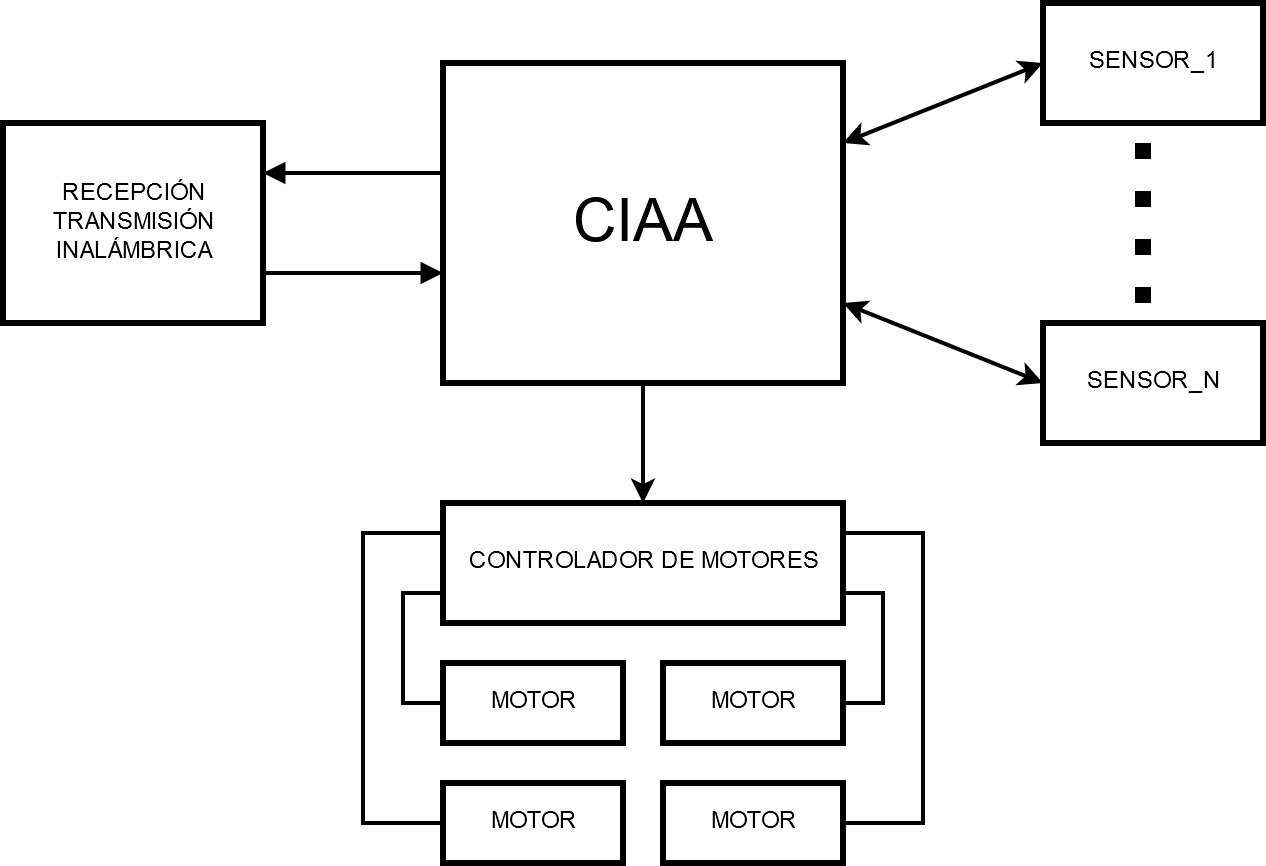
\includegraphics[width=1\linewidth]{informe_1/diagrama_bloque}
{
	\centering\textit{Figura 1. Diagrama en bloques del sistema}

}

\paragraph{Estructura física del vehículo}
El desarrollo del vehículo implica tener una estructura sobre la cual se puedan montar los motores con sus respectivos controladores, sensores, la EDU-CIAA y la/s baterías necesarias para alimentar el sistema. La estructura deberá ser lo suficientemente rígida para soportar el peso del hardware mencionado anteriormente, y al mismo tiempo debe ser liviana para que los motores puedan transportarla sin la necesidad de una potencia excesiva.

\paragraph{Control de Motores}
Los motores deben permitir el movimiento en ambos sentidos, de manera de rotar el vehículo sin utilizar un complejo sistema de servos y bisagras. Los controladores se encuentran sobre el poncho, con salidas para cada motor, haciendo el sistema independiente de los motores y estructura del vehículo, como se puede observar en la \textit{Figura 1}.

\paragraph{Control Remoto}
El objetivo es controlar el vehículo de manera remota a través de protocolo bluetooth. Debe permitir manejar el vehículo desde una distancia considerable (entre 10m y 20m), permitiendo realizar todos los movimientos: avanzar, retroceder, y girar hacia izquierda y derecha. También es deseable disponer de comandos auxiliares para agregar funcionalidad adicional, como por ejemplo, encender/apagar luces manualmente.

\paragraph{Medición de sensores y respuesta en consecuencia}
Como objetivos secundarios del proyecto, consideramos la colocación de algunos sensores: 
\begin{itemize}
	\item Sensor LDR, el cual ante la ausencia de luz se encienden luces delanteras y traseras del vehículo
	\item Sensores de proximidad por infrarrojo, los cuales controlan  el vehículo ante los obstáculos con los que se encuentre
\end{itemize}

	
	% 3
	\chapter{Requerimientos}

\vspace{12pt}
Aquellos requerimientos indicados con \textbf{OPT} son completamente opcionales.

\section{Requerimientos Funcionales}

\subsection{Requerimientos de Software}

\subsubsection{Control de Motores}

\begin{enumerate}
	\item El sistema debe accionar 4 motores individualmente, permitiendo girar en ambas direcciones
	\item El sistema debe accionar motores en conjunto, permitiendo avanzar, retroceder y girar
	\item El sistema debe permitir el bloqueo de movimiento en una dirección (por ejemplo debido a un obstáculo detectado por el sensor de proximidad)
	\item \textbf{OPT} El sistema debe indicar mediante una serie de LEDs el estado de movimiento del vehículo
\end{enumerate}

\subsubsection{Control Remoto}

\begin{enumerate}
	\item El sistema debe  establecer una conexión bluetooth con el sistema de control remoto
	\item El sistema debe leer las indicaciones del control remoto y ejecutar las acciones correspondientes
	\item El sistema debe indicar mediante un LED el estado de la conexión bluetooth
\end{enumerate}

\subsubsection{\textbf{OPT} Medición Sensores }

\begin{enumerate}
	\item Ante ausencia de luz externa, se deben encender las luces del vehículo
	\item Ante la presencia de obstáculos, se debe frenar el desplazamiento en esa dirección
	
\end{enumerate}

\subsection{Requerimientos de Hardware}

\subsubsection{Control de Motores}

\begin{enumerate}
	\item El vehículo debe utilizar puentes H para motores de corriente continua
	\item \textbf{OPT} El vehículo debe Indicar con un LED para cada motor si este está en movimiento
\end{enumerate}

\subsubsection{Baterías y cargador}

\begin{enumerate}
	\item El vehículo debe utilizar baterías de Litio para lograr la autonomía del vehículo
	\item El vehículo debe indicar mediante un LED cuando haya baja tensión
	\item El vehículo debe permitir cargar las baterías mediante un puerto USB
\end{enumerate}

\subsubsection{Componentes}

\begin{enumerate}
	\item Se debe contar con una llave de encendido/apagado y un LED que determine su estado
	\item \textbf{OPT} El sistema debe poseer un buzzer para indicar eventos o fallas
\end{enumerate}

\section{Requerimientos No Funcionales}

\begin{itemize}
	\item Utilización de la placa de desarrollo EDU-CIAA
	\item Estructura sólida y liviana, donde se colocan los motores y la EDU-CIAA
	\item El conexionado a los motores debe ser a través de borneras para poder cambiar la estructura.
	\item Programación en lenguaje C
	\item Desarrollo de PCB en formato de poncho
	\item Mecanismo de control simple
	\item El sistema debe manejar respuestas en tiempo real.
	\item Fecha de finalización y entrega del proyecto el día 16/12
	
\end{itemize}

	
	% 4
	\chapter{Diseño de Hardware}

\section{Diagrama en Bloques}

\subsection{Recepción Inalámbrica}

\paragraph{}
Para implementar el manejo por control remoto se utiliza el protocolo Bluetooth, 
más especificamente el módulo HM-10, que funciona como una comunicación serie
inalámbrica. Del lado del usuario se utiliza la aplicación de Android
"BLEJoystick", disponible en Google Play Store. También se cuenta con un LED
para indicar la correcta vinculacion entre la app y el módulo bluetooth.

\subsubsection{Componentes a Utilizar}

\begin{longtable}[]{|c|c|c|c|p{3.2cm}|c|}
	\toprule
	Componente & Código & Valor & Cantidad & Función &
	Protocolo\tabularnewline
	\midrule
	\endhead
	Rx/Tx BLE & HM-10 & - & 1 & Recepción & UART
	8N1\tabularnewline
	LED & - & Rojo 3mm & 1 & Informar estado\newline de la conexión Bluetooth &
	Digital\tabularnewline
	\bottomrule
\end{longtable}

\subsubsection{Rx/Tx BLE}

\begin{figure}[H]
	\centering
	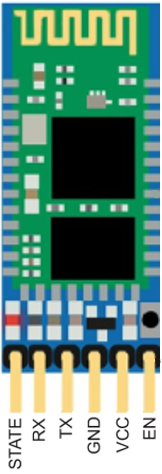
\includegraphics[width=0.15\linewidth]{informe_2/encapsulado_HM-10}
	\caption{HM-10}
	\label{fig:encapsuladohm-10}
\end{figure}


\paragraph{}El módulo Bluetooth a utilizar es el HM-10 provisto por la cátedra, el cual ya
fue utilizado en asignaturas anteriores por lo cual se conocen sus características 
y su funcionamiento.
Además, la sAPI de la CIAA provee una librería para comunicación Bluetooth, facilitando 
su programación.

\paragraph{}Respecto a las características de Hardware, el HM-10 funciona a 3.3v, por lo que
no hay que realizar ninguna adaptación para su funcionamiento.

\subsubsection{LED}

\paragraph{}Para la alimentación del LED se utiliza el puerto GPIO1, realizando los 
siguientes cálculos se obtiene el valor de la resistencia que necesita 
para su conexión::


$$ \mathrm{R} = \frac{\mathrm{V} - \mathrm{LED_V}}{\mathrm{LED_I}} = 420\Omega $$

$ \mathrm{V} = 3.3\mathrm{v};\ \mathrm{LED_V} = 1.2\mathrm{v};\ \mathrm{LED_I} = 5\mathrm{mA};  $

\subsubsection{Conexionado}

\paragraph{HM-10} El módulo Bluetooth se comunica a través de un protocolo serie 8N1,
a 9600 bps, y se configura a través de comandos AT. Las librerías de la CIAA
ya proveen funciones para establecer una comunicación con un módulo HM-10.

\paragraph{LED}Se conecta de manera directa a una salida digital del integrado, 
teniendo en cuenta la resistencia mencionada.

\subsubsection{Esquemático}

\begin{figure}[H]
	\centering
	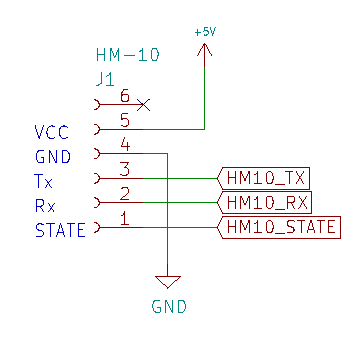
\includegraphics[width=0.5\linewidth]{informe_3/schem_hm10}
	\caption{Conexionado del Módulo Bluetooth HM-10}
	\label{fig:schemhm10}
\end{figure}

\begin{figure}[H]
	\centering
	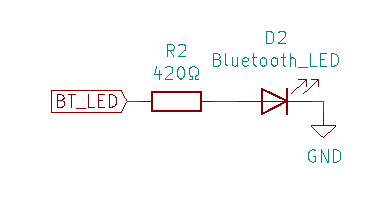
\includegraphics[width=0.5\linewidth]{informe_3/schem_bt_led}
	\caption{Conexionado del LED Bluetooth}
	\label{fig:schemledbt}
\end{figure}

\subsection{Controlador de Motores}

\paragraph{}Para el control de motores se utiliza el circuito integrado L293D, en nuestro 
caso utilizamos la versión de STMicroelectronics, el cual provee dos puente H completos,
permitiendo así controlar hasta dos motores en ambos sentidos.

\subsubsection{Componentes a Utilizar}

\begin{longtable}[]{|c|c|c|c|p{3.2cm}|c|}
	\toprule
	Componente & Código & Valor & Cantidad & Función &
	Protocolo\tabularnewline
	\midrule
	\endhead
	Puente H & L293D & - & 2 & Controlar motores &
	Analógico/PWM\tabularnewline
	\bottomrule
\end{longtable}

\subsubsection{Puente H}

\begin{figure}[H]
	\centering
	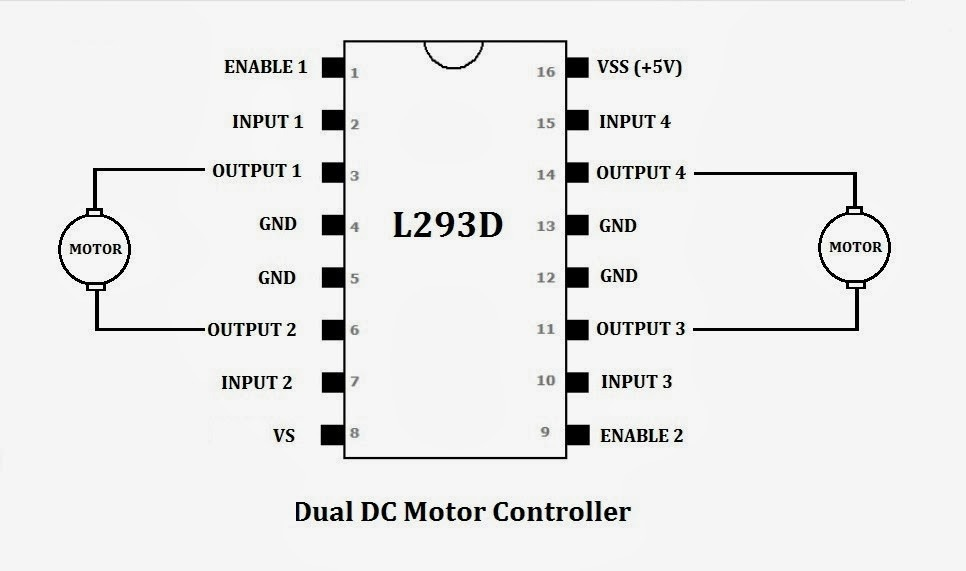
\includegraphics[width=0.7\linewidth]{informe_2/encapsulado_L293D}
	\caption{L293D}
	\label{fig:encapsuladol293d}
\end{figure}

\paragraph{}Al investigar sobre circuitos que provean puentes H para controlar motores de
continua, rápidamente encontramos el L293D. Este tiene 4 canales, cada uno
formando medio puente H. Dado que para girar motores en ambos sentidos se
requiere un puente completo, se pueden controlar dos motores con un solo
L293D.

En términos de conexionado provee un \emph{enable} por cada par de canales,
alimentación independiente para lógica y motores, y 6 pines centrales para
disipación de calor.

Respecto a la alimentación, requiere entre 4.5v y 30v. Dado el elevado consumo
es imposible alimentarlo directamente a través de la CIAA, por lo que se conecta  
de manera directa a la fuente de alimentación.

Soporta corrientes pico de 1.2A, por lo que es correcto colocar un disipador en
caso de que los motores consuman mucha corriente.

\subsubsection{Conexionado}

\paragraph{L293D}Las entradas de los L293D se controlan mediante PWM, permitiendo
controlar la velocidad de cada motor de manera independiente. Esto requiere
utilizar 8 PWM, dos para cada motor.

\subsubsection{Esquemático}

\begin{figure}[H]
	\centering
	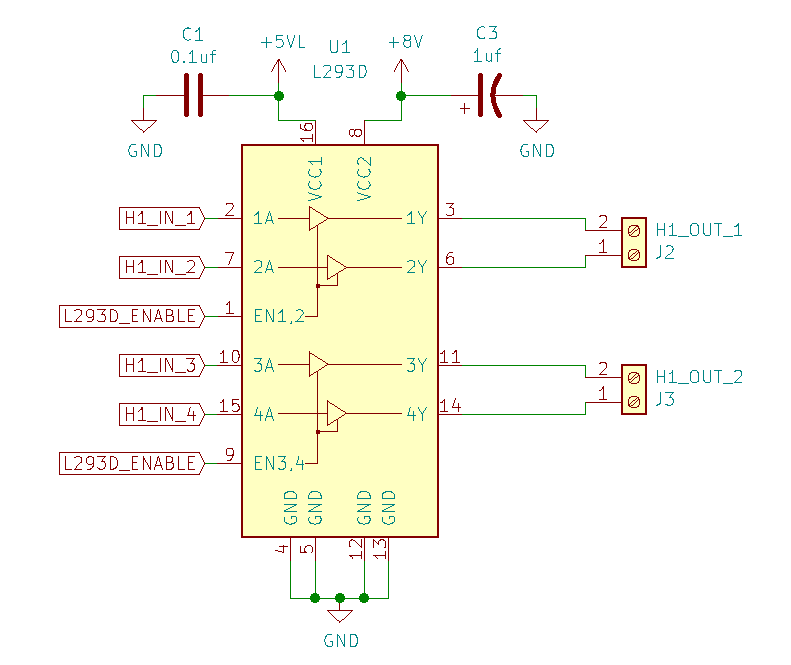
\includegraphics[width=0.7\linewidth]{informe_3/schem_L293D}
	\caption{Conexionado de un L293D}
	\label{fig:scheml293D}
\end{figure}

\paragraph{Capacitores} Se colocan capacitores en la alimentación según indica la hoja de datos del integrado L293D de Texas Instruments.

\subsection{Detector de Obstáculos}

\paragraph{} Para detectar obstáculos se utiliza el sensor de proximidad de Arduino
HC-SR04, que permite captar objetos entre 2cm y 400cm, con un ángulo de \ang{15}. 
Estos rangos resultan ideales para detectar obstáculos y actuar en consecuencia
en un vehículo a control remoto.

\subsubsection{Componentes a Utilizar}

\begin{longtable}[]{|c|c|c|c|p{3.2cm}|c|}
	\toprule
	Componente & Código & Valor & Cantidad & Función &
	Protocolo\tabularnewline
	\midrule
	\endhead
	Sensor Proximidad & HC-SR04 & - & 1 & Medir distancia a obstáculos &
	Digital\tabularnewline
	Buzzer & - & - & 1 & Indicar mediante sonido & Digital\tabularnewline
	\bottomrule
\end{longtable}

\subsubsection{Sensor de Proximidad}

\begin{figure}[H]
	\centering
	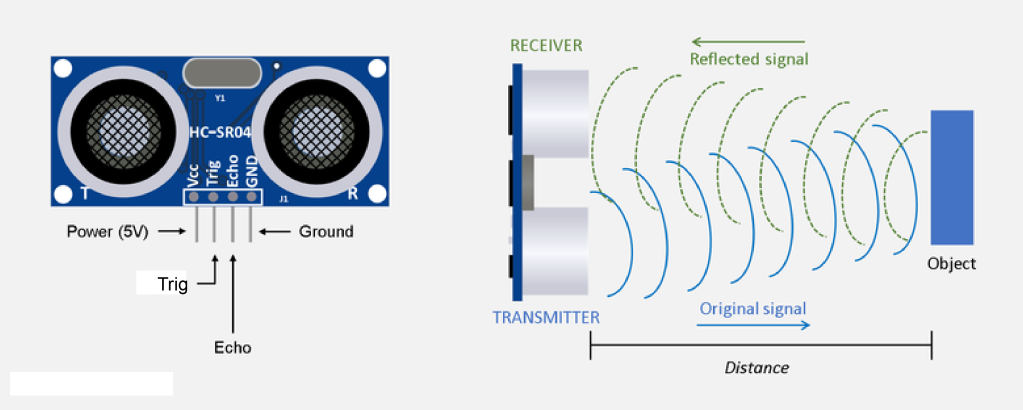
\includegraphics[width=0.7\linewidth]{informe_2/encapsulado_HC-SR04}
	\caption{HC-SR04}
	\label{fig:encapsuladohc-sr04}
\end{figure}

\paragraph{}El HC-SR04 es un sensor ultrasónico que permite calcular la distancia de los
objetos que se encuentran en frente a él, con un ángulo de visión de \ang{15}. 
Utiliza una onda sonora de 40kHz, inaudible para el oido humano, que se emite
cuando se coloca un 1 en el pin \emph{trigger}. Cuando el módulo detecta el rebote 
del pulso emitido, coloca un 1 en el pin \emph{echo}. Midiendo el tiempo entre la 
emisión del pulso y la recepción del eco, puede determinarse la distancia al objeto.

\subsubsection{Buzzer}
\paragraph{}Se utiliza como componente auxiliar para indicar la presencia de obstáculos mediante sonido.

\subsubsection{Conexionado}

\paragraph{HC-SR04} Dado que requiere medir con presición el tiempo transcurrido, es
necesario utilizar un timer en modo \emph{input capture} para lograr la
mayor presición posible. El \emph{trigger} se generará con una salida
GPIO común.

\paragraph{Buzzer}Dado que el consumo del buzzer supera el máximo tolerado por los puertos GPIO de la CIAA, 
se utiliza un transistor para alimentar el buzzer y asegurar su correcto funcionamiento
sin dañar ningún componente de hardware. Se utiliza el pin de GPIO7 como salida para el LED.

\subsubsection{Esquemático}

\begin{figure}[H]
	\centering
	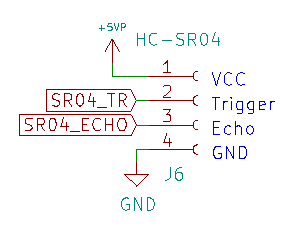
\includegraphics[width=0.4\linewidth]{informe_3/schem_hcsr04}
	\caption{Conexionado del HC-SR04}
	\label{fig:schemhcsr04}
\end{figure}

\begin{figure}[H]
	\centering
	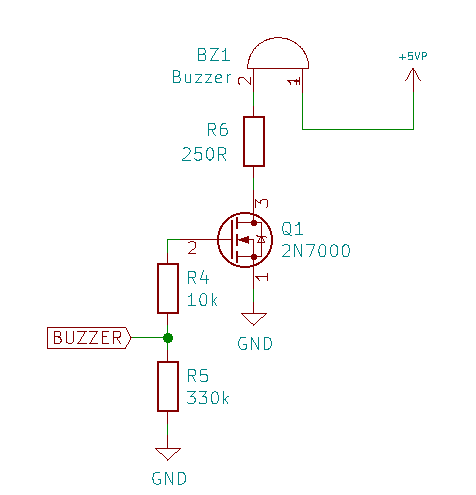
\includegraphics[width=0.5\linewidth]{informe_3/schem_buzzer}
	\caption{Conexionado del Buzzer}
	\label{fig:schembuzzer}
\end{figure}

\subsection{Indicadores de Estado}

\paragraph{}Se utiliza como componente auxiliar para indicar el estado del vehículo, un LED que indica si el vehículo está encendido.

\subsubsection{Esquemático}

\begin{figure}[H]
	\centering
	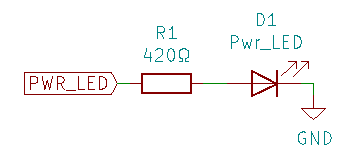
\includegraphics[width=0.4\linewidth]{informe_3/schem_pwr_led.png}
	\caption{Conexionado del LED de encendido}
	\label{fig:schempwrled}
\end{figure}

\section{Cálculos de Corriente}

\begin{longtable}[]{|c|c|c|}
	\toprule
	Subsistema & Tensión {[}V{]} & Corriente {[}mA{]}\tabularnewline
	\midrule
	\endhead
	Principal & 5 & 200\tabularnewline
	UART2 (BT) & - & 0.5\tabularnewline
	SCT * 3 & - & 0.16 *3\tabularnewline
	GPIO * 6 & - & 5 * 6\tabularnewline
	HM-10 & 5 & 10\tabularnewline
	L293D * 2 & 5 & 32 * 2\tabularnewline
	Motor * 4 & 8 & 100 * 4\tabularnewline
	------------- & ------------- & -----------------\tabularnewline
	\textbf{Total} & 5 & 280mA\tabularnewline
	\textbf{Total} & 8 & 400mA\tabularnewline
	\bottomrule
\end{longtable}

\paragraph{}Como se puede observar, dado la variedad de dispositivos y componentes,
se requieren dos valores de tensión diferentes. Además, al tratarse de un vehículo
manejado inalámbricamente, es necesario el uso de baterías. Utilizando dos baterías de Litio en serie 
se obtiene una tensión de entrada de aproximadamente 8V, por lo tanto, es necesario utilizar un conversor DC-DC 
step-down para obtener tensiones de 5V, y el conversor interno de la EDU-CIAA para obtener tension de de 3.3V.

Para alimentar la EDU-CIAA se opta por utilizar el conector Molex de alimentación externa, utilizando uno
igual en el poncho.

\subsubsection{Esquemático}

\begin{figure}[H]
	\centering
	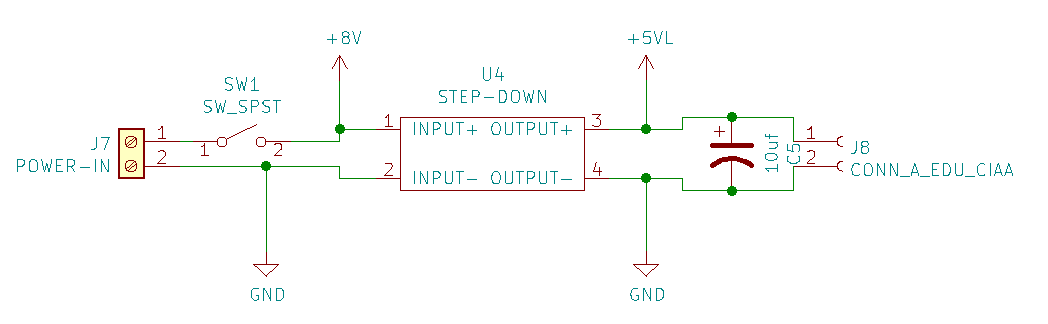
\includegraphics[width=0.8\linewidth]{informe_3/schem_fuente}
	\caption{Conexionado de la alimentación}
	\label{fig:schemfuente}
\end{figure}


\section{Diseño de PCB}

\paragraph{}Para el diseño de la PCB se tuvieron en cuenta las siguientes características:

\begin{itemize}
	\item Los conectores para los motores se deben disponer de manera que representen la rueda que está accionando.
	\item Los integrados L293D deben alejarse del resto de los componentes, ya que manejan una elevada corriente, y mucha temperatura.
	\item Los integrados L293D deben tener un plano de tierra en sus pines centrales, tal como indica  la hoja de datos, para poder disipar calor.
	\item El sensor ultrasonido HC-SR04 debe encontrarse en un extremo de la placa, de manera que la PCB pueda montarse con este sensor apuntando hacia adelante.
	\item El conector de baterías debe colocarse cerca de los extremos para no tener cables muy largos.
	\item El conector de alimentación para la EDU-CIAA debe encontrarse lo más cerca posible del conector en la EDU-CIAA.
	\item Tener en cuenta las recomendaciones de la cátedra respecto al ancho de pista, y distancia entre estas. Como así también el tamaño de los pads.
\end{itemize}

\subsection{Ancho de pistas}

\paragraph{} Además, debe tenerse en cuenta que dado el elevado consumo de los motores, es necesario tener en cuenta el ancho de las pistas, para no sobrecalentarlas. Utilizando la calculadora incorporada en KiCAD, se ve que una pista de 0.6mm (lo mínimo recomendado por la cátedra) puede tolerar sin problemas hasta 1.6A, por lo qué para todas las aplicaciones de GPIO, PWM, y alimentación de periféricos no hay problemas.

\paragraph{}Respecto a los L293D, están diseñados para soportar 300mA por canal, con una corriente máxima total de 1.2A, por lo qué, tanto las pistas de los motores como las de alimentación no requieren más que el ancho mínimo de 0.6mm. Sin embargo hay que tener en cuenta que el consumo de ambos combinados puede llegar a 2.4A, por lo que, la pista ``compartida'' de alimentación, si debe tener un ancho mayor, calculado en 1mm.

\paragraph{}El consumo total de la placa se estipula en 3A, dado que la CIAA consume alrededor de 200mA, y los motores 2.4A en los casos más extremos. Los consumos se resumen en la siguiente tabla:

\begin{longtable}[]{|c|c|c|c|}
	\toprule
	Pista & Consumo & Ancho real & Ancho a utilizar \tabularnewline
	\midrule
	Alimentación L293D & 1.3A & 0.4mm & 0.6mm \tabularnewline
	Alimentación de 2 L293D & 2.6A & 1mm & 1mm\tabularnewline
	8v (total) & 3A & 1.3mm & 1.3mm\tabularnewline
	5v & 0.4A & 0.08mm & 0.6mm\tabularnewline
	\endhead
	
	\bottomrule
\end{longtable}

Nota: para los cálculos finales, se agregó un 10\% de consumo por seguridad. Además, los cálculos para los L293D se realizan en base a las capacidades máximas de los mismos, y no con los motores que se disponen, que tienen un consumo mucho menor.

\subsection{Consideraciones para cada dispositivo}

Se trató de agrupar físicamente los componentes según su asociación lógica. Por ejemplo, las resistencias para un LED, cerca de ese LED.

\paragraph{L293D} Además de los requisitos mencionados previamente para los puentes H, debe tenerse en cuenta que requieren de capacitores filtro en las entradas de alimentación, cerca de cada integrado.

\subsection{BOM simplificado}

A continuación se presenta una versión simplificada de la lista de materiales en un formato legible, para un BOM más detallado que incluya las footprints de KiCAD, ver Anexo.


\begin{longtable}[]{|c|c|p{7cm}|}
	\toprule
	Referencia & Valor & Componente \tabularnewline
	\midrule
	\endhead
	
	BZ1 & - & Buzzer 12x9.5x7.6\tabularnewline
	C1 & 100nF & Capacitor cerámico\tabularnewline
	C2 & 100nF & Capacitor cerámico\tabularnewline
	C3 & 1uF & Capacitor electrolítico\tabularnewline
	C4 & 1uF & Capacitor electrolítico\tabularnewline
	C5 & 10uF & Capacitor electrolítico\tabularnewline
	D1 & LED 5mm & LED 5mm\tabularnewline
	D2 & LED 5mm & LED 5mm\tabularnewline
	D3 & LED 5mm & LED 5mm\tabularnewline
	J1 & Header HM10 & Tira de pin hembra x6\tabularnewline
	J2 & - & Bornera Azul de 2\tabularnewline
	J3 & - & Bornera Azul de 2\tabularnewline
	J4 & - & Bornera Azul de 2\tabularnewline
	J5 & - & Bornera Azul de 2\tabularnewline
	J6 & Header HC-SR04 & Tira de pin hembra x4\tabularnewline
	J7 & - & Bornera Azul de 2\tabularnewline
	J8 & - & Molex KK254 Macho 2 pines\tabularnewline
	Q1 & 2n7000 & Transistor 2n7000\tabularnewline
	R1 & 420R & Resistencia carbón 1/4\tabularnewline
	R2 & 420R & Resistencia carbón 1/4\tabularnewline
	R3 & 420R & Resistencia carbón 1/4\tabularnewline
	R4 & 10k & Resistencia carbón 1/4\tabularnewline
	R5 & 330k & Resistencia carbón 1/4\tabularnewline
	R6 & 250R & Resistencia carbón 1/4\tabularnewline
	SW1 & Switch SPST & Interruptor DIP 1 posición\tabularnewline
	U1 & L293D & Puente H L293D\tabularnewline
	U2 & L293D & Puente H L293D\tabularnewline
	U4 & Mini360 & Fuente Step-Down mini360\tabularnewline
	X & Pines & Tira de pines p/edu-ciaa\tabularnewline
	N/A & HM-10 & HM-10\tabularnewline
	N/A & HC-SR04 & HC-SR04\tabularnewline	
	
	\bottomrule
\end{longtable}

	
	% 5
	\chapter{Diseño de Software}

\paragraph{}
Se optó por utilizar una arquitectura Time-Triggered cooperativa, donde
las tareas se corresponden con los subsistemas de Hardware:

\begin{itemize}
	\item
	Control de motores
	\item
	Recepción inalámbrica
	\item
	Detector de obstáculos
\end{itemize}

Además de la interrupción de tiempo, propia de la arquitectura Time
Triggered, se necesita una interrupción de tiempo independiente
utilizada por el sensor de proximidad para medir con presición la
distancia a la que se encuentran los obstáctulos.

El psuedocódigo del programa principal se resume a lo siguiente:

\begin{Verbatim}
interrupcion 50ms:
	flag_tiempo = 1

variables compartidas:
	accion_vehiculo # Enumerativo que indica el desplazamiento que
			# se debe realizar


programa principal:
	inicializacion motores
	inicializacion bluetooth
	inicializacion detector de colisiones
	prender led power

super loop:
	si flag_tiempo = 1:
		leer bluetooth
		detectar colisiones
		actualizar motores
		flag_tiempo = 0
\end{Verbatim}


\section{Pseudocódigo de los Módulos}

\subsection{Leer Bluetooth}

\begin{Verbatim}
si hay mensajes nuevos:
	leer el mensaje
	si es una A o a:
		motor = avance
	si es una C o C:
		motor = retrocede
	si es una D o d:
		motor = giro izquierda
	si es una B o b:
		motor = giro derecha
	si es un 0:
		motor = giro libre
	si es una F o f:
		motor = freno
\end{Verbatim}

\subsection{Detectar Colisiones}

\paragraph{}El eco producido por el módulo se genera -aproximadamente- entre 60uS y
12mS. Creemos que no es necesario realizar las mediciones cada estos
periodos tan cortos de tiempo, dado que, puede ser contraproducente para
los tiempos del sistema considerando el objetivo del sensor. Por esto,
el procesamiento del se realiza cada 250ms:

\begin{Verbatim}
inicializar detector de colisiones:
	tick_colision = 0

detectar colisiones:
	tick_colision++
	si tick_colision = 5:
		tick_colision = 0
		tomar tiempo
		prender input capture
		enviar señal de comienzo de medicion

si llego el echo:
	calcular distancia
	si hay un obstaculo cerca:
		bloquear movimiento hacia adelante
\end{Verbatim}

\subsection{Actualizar Motores}

\paragraph{} Los motores se controlan en dos niveles: a bajo nivel se puede controlar cada
motor de manera independiente, indicando la dirección de giro. Una capa
más ``alta'' permite controlar el vehículo más facilmente, brindando
funciones para indicar como se debe mover el vehículo.

\begin{figure}[H]
	\centering
	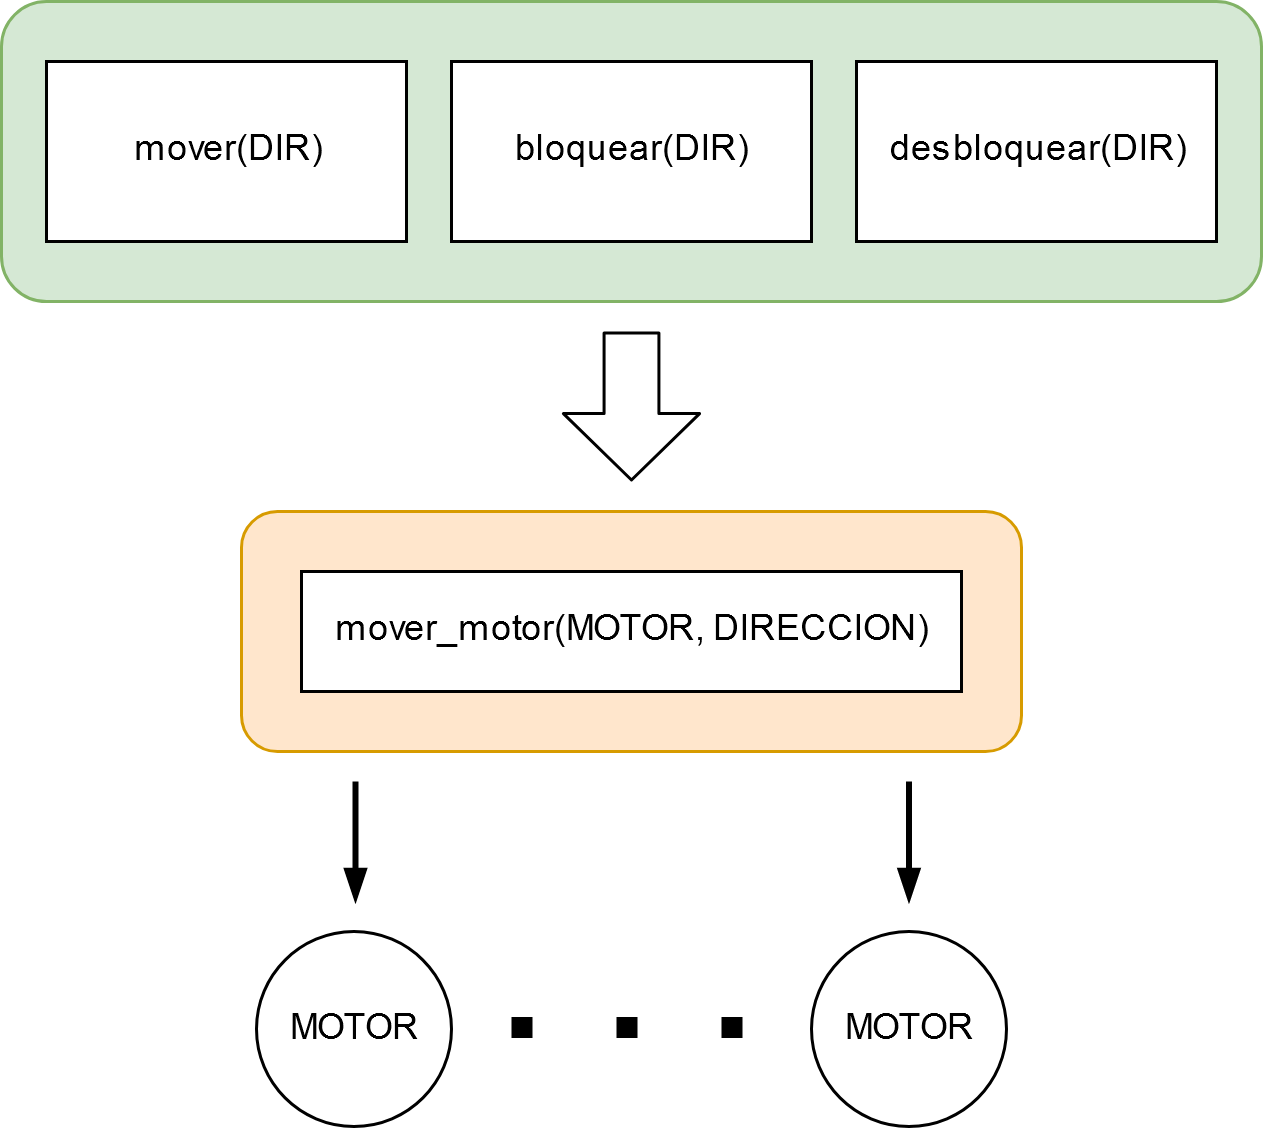
\includegraphics[width=0.5\linewidth]{informe_2/capas_motor}
	\caption{Capas de los Motores}
	\label{fig:capasmotor}
\end{figure}


Por lo que el pseudocódigo se reduce a lo siguiente

\begin{Verbatim}
inicializacion de motores:
	setear movimiento en libre

actualizacion de motores:
	ver accion_vehiculo
	mover el vehiculo en la direccion solicitada

	# A modo de ejemplo se explica como mover en una sola direccion
	si movimiento es hacia adelante:
		motor trasero izquierdo girar horario
		motor trasero derecho girar antihorario
		motor delantero izquierdo girar horario
		motor delantero derecho girar horario
	...
\end{Verbatim}

A bajo nivel se controla cada motor individualmente:

\begin{Verbatim}
si movimiento es horario:
	colocar canal 1 en alto
	colocar canal 0 en bajo
si movimiento es anti horario:
	colocar canal 0 en bajo
	colocar canal 1 en alto
\end{Verbatim}

\subsection{Software Android}

\paragraph{BLEJoystick}
BLEJoystick es la aplicación a utilizar para el control inalámbrico del
vehículo, está disponible para múltiples dispositivos android y se puede
descargar de manera gratuita desde Google Play Store. Esta aplicación se
conecta al módulo bluetooth HM-10 mediante el protocolo bluetooth low
energy 4.0 (BLE). Cuenta con 8 botones, donde el funcionamiento de cada
uno es el siguiente: 

\begin{itemize}
	\item
	Cuando se presiona por primera vez, envía una letra en mayúscula.
	\item
	Mientras siga presionado el mismo botón, envía la misma letra en
	minúscula de manera constante.
	\item
	Cuando se suelta el boton, envía un 0.
\end{itemize}

A continuación se describe cada uno de los botones y su letra
correspondiente:

\begin{longtable}[]{@{}lll@{}}
	\toprule
	Botón & Letra inicial & Letra constante\tabularnewline
	\midrule
	\endhead
	Arriba & A & a\tabularnewline
	Derecha & B & b\tabularnewline
	Abajo & C & c\tabularnewline
	Izquierda & D & d\tabularnewline
	Triángulo & E & e\tabularnewline
	Círculo & F & f\tabularnewline
	Equis & G & g\tabularnewline
	Cuadrado & H & h\tabularnewline
	\bottomrule
\end{longtable}

\section{Interfaz de Usuario}

\subsection{Pasos a seguir para la configuración del sistema}

\begin{figure}[H]
	\centering
	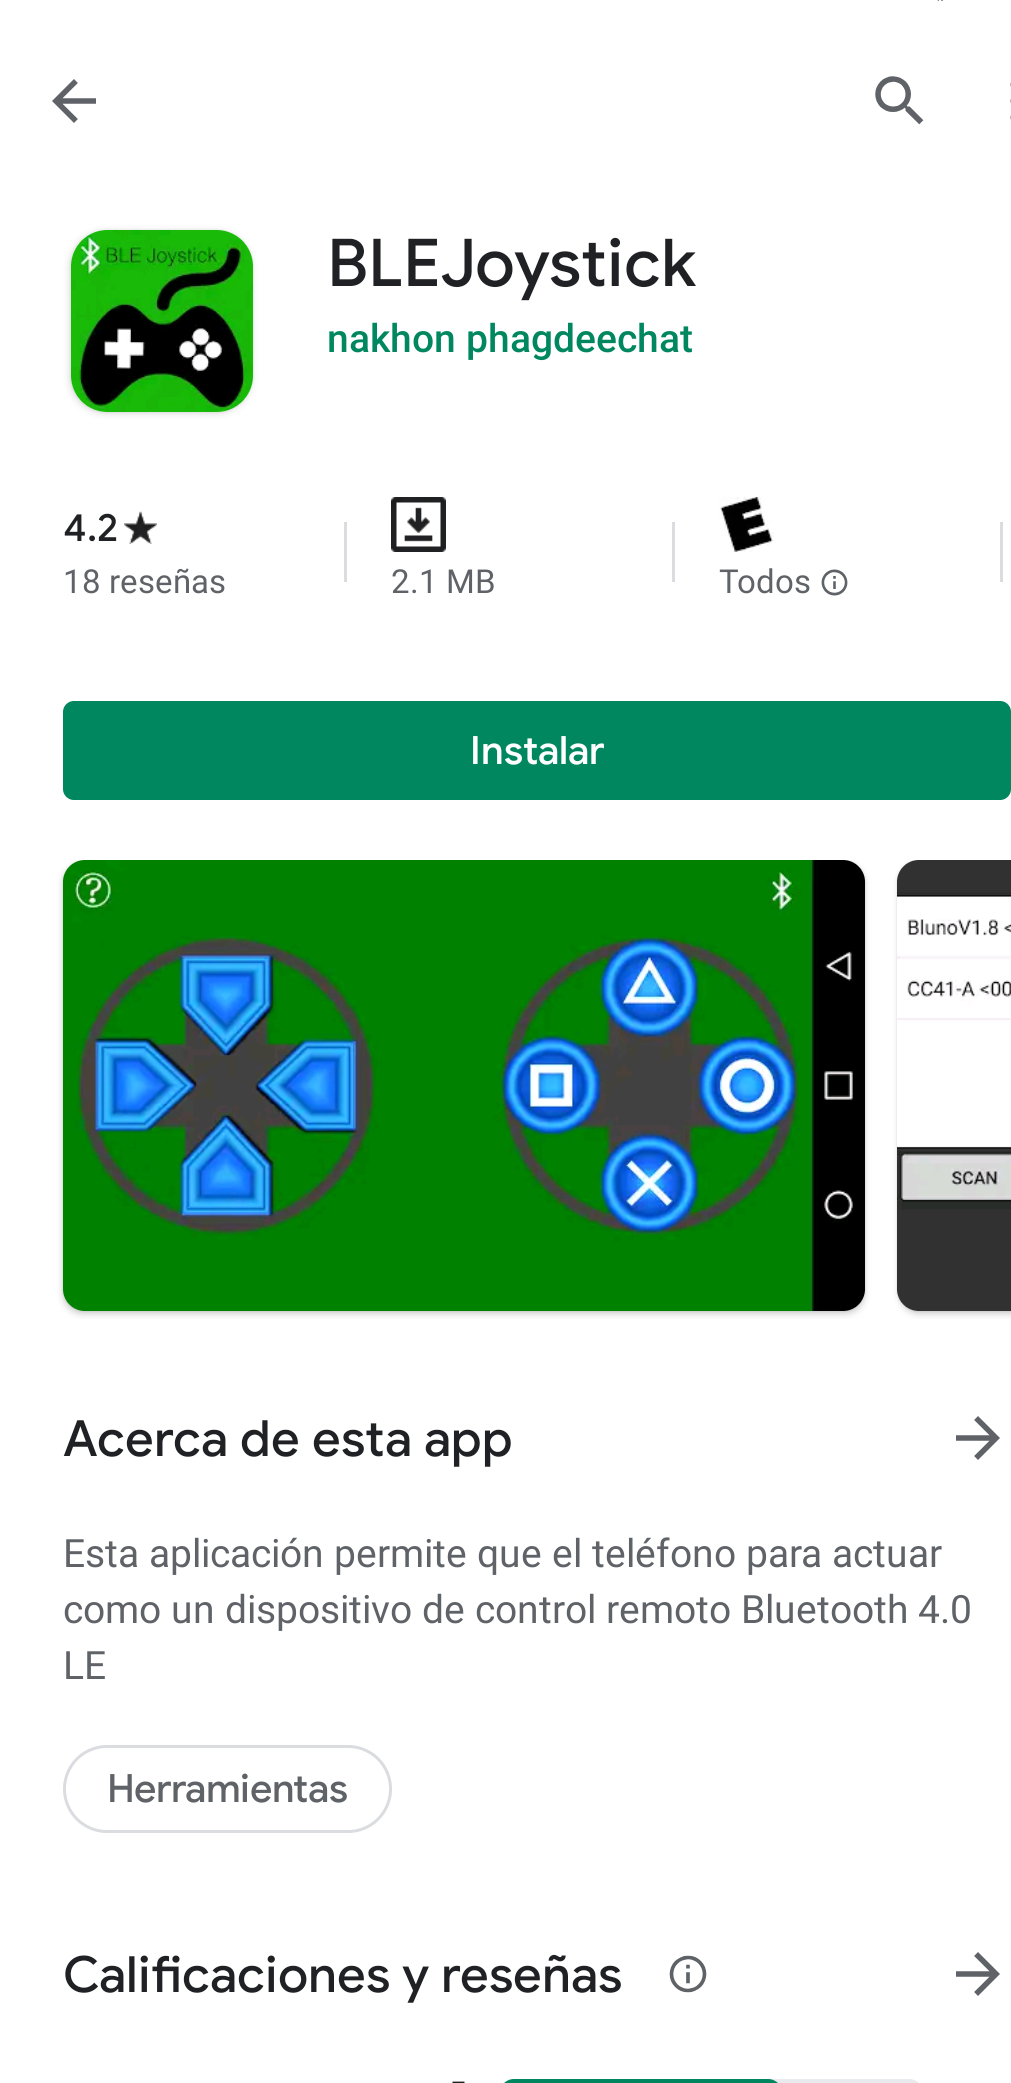
\includegraphics[width=0.5\linewidth]{informe_2/interfaz_joystick_store}
	\caption{Aplicación en el Play Store}
	\label{fig:interfazjoystickstore}
\end{figure}

\begin{enumerate}
	\def\labelenumi{\arabic{enumi}.}
	\item
	Ingresar a Google Play Store
	\item
	Descargar la aplicación BLEJoystick
	\item
	Iniciar la aplicación.
	\item
	Pulsar el ícono de vinculación bluetooth y seleccionar
	\emph{vehiculo}.
	\item
	Corroborar la correcta vinculación mediante el LED indicador.
	\item
	Sistema listo para usar.
\end{enumerate}

\subsection{Utilización del Vehículo}

\begin{figure}[H]
	\centering
	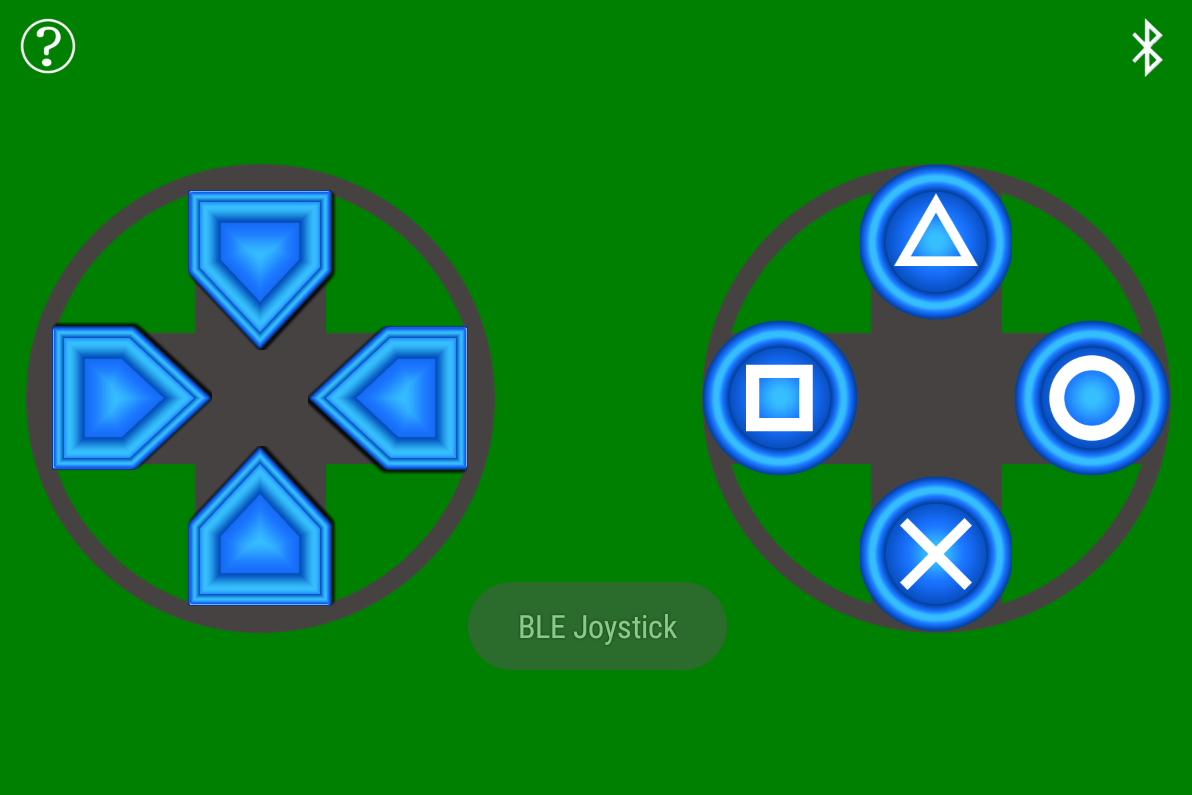
\includegraphics[width=0.7\linewidth]{informe_2/interfaz_joystick}
	\caption{La aplicación BLEJoystick}
	\label{fig:interfazjoystick}
\end{figure}

A continuación se detalla y explica el funcionamiento 
de cada uno de los botones disponibles en la aplicación
\begin{longtable}[]{@{}ll@{}}
	\toprule
	Botón & Función\tabularnewline
	\midrule
	\endhead
	Arriba & Desplazar hacia adelante\tabularnewline
	Derecha & Girar hacia la derecha\tabularnewline
	Abajo & Desplazar hacia abajo\tabularnewline
	Izquierda & Girar hacia la izquierda\tabularnewline
	Círculo & Frenar\tabularnewline
	\bottomrule
\end{longtable}

\section{Librerías de Software}

\paragraph{sAPI} Dada la extensión de la librería provista por la CIAA, solo se requiere
usar esta. Más específicamente se utilizaran las librerías
\texttt{sapi\_pwm.h}, \texttt{sapi\_gpio.h}
y \texttt{sapi\_timer.h}.

\section{Ensayos}

\subsection{Motores y L293D}

\paragraph{}Realizamos una prueba de los motores con los L293D, para esto realizamos un prototipo de la estructura del vehículo con el objetivo de observar el correcto funcionamiento tanto de los motores como del chip L293D y verificar si la potencia de los motores será suficiente para mover el vehículo con todos sus componentes a una velocidad considerable. 

El ensayo se realizó con una placa de Arduino con un shield para controlar motores, donde todos los motores fueron configurados con la máxima velocidad posible, generando el siguiente el código de prueba:

\begin{lstlisting}[language=C,basicstyle=\footnotesize\ttfamily]

#include <AFMotor.h>

AF_DCMotor motor1(1);	// Declara los motores a utilizar
AF_DCMotor motor2(2);
AF_DCMotor motor3(3);
AF_DCMotor motor4(4);

void setup() {
	Serial.begin(9600);	// Inicializa la terminal serie a 
						// 9600 bps
	Serial.println("Prueba de motores");


	motor1.run(RELEASE);	// Desbloquea el motor
	motor1.run(FORWARD);    // Mueve para adelante
	motor1.setSpeed(255);   // Velocidad entre 0 y 255,
                            // configurada al maximo
	
	motor2.run(RELEASE);
	motor2.run(FORWARD);
	motor2.setSpeed(255);
	
	motor3.run(RELEASE);
	motor3.run(FORWARD);
	motor3.setSpeed(255);
	
	motor4.run(RELEASE);
	motor4.run(FORWARD);
	motor4.setSpeed(255);
}

void loop() {
}
\end{lstlisting}

\paragraph{Conclusiones} Los motores son lo suficientemente potentes como para mover el vehículo a una velocidad considerable, siempre y cuando los L293D sean alimentados con aproximadamente 8V, ya que hay una diferencia entre la entrada del L293D y la salida a cada uno de los motores de ~=2V (los motores van a su máxima velocidad con 6V).

\subsection{PWM}

\paragraph{} Para el análisis preliminar de PWM, se utilizó como código de prueba el ejemplo \verb|pwm_dimmer|. Dicho código utiliza la modulación de ancho de pulso para variar la intensidad de los LEDs alojados en la placa de la EDU CIAA.  A partir de dicho análisis se determinó la necesidad de configurar las correspondencias entre los canales del SCT con los pines del microcontrolador, ya que el proyecto requiere un total de 8 salidas PWM y con la configuración por defecto no eran suficientes; los canales asociados a  CTOUT2, CTOUT4 y CTOUT5 están vinculados a los pines P2\_10, P2\_11 y P\_12 correspondientes a los leds de la placa, dicha relación se establece en el archivo \verb|sapi\_sct.c| ubicado en las librerías del firmware v3 correspondientes a la sAPI. La modificación requerida consiste en derivar la salida del CTOUT2 a LCD1 de la siguiente manera:

\begin{lstlisting}[language=c,basicstyle=\footnotesize\ttfamily]
static pinInitLpc4337_t SCTdataList[] = {

// Configuracion por default:
...
/* Sct n | port | pin | name in board */
/* CTOUT2 */ { 4 , 10 }, /* LED1 */
...

// Configuracion requerida:
...
/* Sct n | port | pin | name in board */
/* CTOUT2 */ { 4 , 4 }, /* LCD1 */
...

}
\end{lstlisting}

Finalmente se verificó el correcto funcionamiento corriendo el programa y conectando en el terminal 30 de la placa, indicado como LCD1, un LED con su correspondiente resistencia.
	
	% 6
	\chapter{Ensayos y Mediciones}

\section{Motores y L293D}

Con el objetivo de observar el funcionamiento del L293D, los motores y
verificar si estos eran capaces de mover el vehículo con todos los
componentes a una velocidad aceptable, se realizó un prototipo con un Arduino, una caja de cartón que se utilizó 
como estructura provisoria (ver figura \ref{fig:ensayo1} y \ref{fig:ensayo2}) y el shield que contiene dos L293D, configurando el PWM con un ciclo de trabajo del 100\%. 
Para facilitar el prototipado, se utilizó la librería para control de motores desarrollada por Adafruit. El código de prueba para el Arduino es el siguiente:

\begin{lstlisting}
#include <AFMotor.h>

AF_DCMotor motor1(1);                   //Declara los motores a utilizar
AF_DCMotor motor2(2);
AF_DCMotor motor3(3);
AF_DCMotor motor4(4);

void setup() {
  Serial.begin(9600);                   //Inicializa la terminal serie a 9600 bps
  Serial.println("Prueba de motores");

  motor1.run(RELEASE);                  //Desbloquea el motor
  motor1.run(FORWARD);                  //Mueve para adelante
  motor1.setSpeed(255);                 //Velocidad entre 0 y 255, configurada al máximo

  motor2.run(RELEASE);
  motor2.run(FORWARD);
  motor2.setSpeed(255);

  motor3.run(RELEASE);
  motor3.run(FORWARD);
  motor3.setSpeed(255);

  motor4.run(RELEASE);
  motor4.run(FORWARD);
  motor4.setSpeed(255);
}

void loop() {
}
\end{lstlisting}

\paragraph{Conclusiones}

Los motores son lo suficientemente potentes como para mover el vehículo
a una velocidad considerable, siempre y cuando los L293D sean
alimentados con aproximadamente 8V, ya que hay una diferencia entre la
entrada del L293D y la salida a cada uno de los motores de
aproxidamente 2V (los motores van a su máxima velocidad con 6V).

\section{Sensor HC-SR04}

Una vez ensamblado el auto en su correspondiente chasis en conjunto con
la totalidad de sus componentes, realizamos las pruebas de detección de
objetos. Estas pruebas consistieron en direccionar el auto hacia un
obstáculo, contemplando el margen de frenado requerido para que el
vehículo no choque contra dicho obstáculo, realizando sucesivas
modificaciones en las variables de distancia de frenado hasta dar con la
indicada. El código en cuestión se muestra a continuación:

\begin{lstlisting}
void evaluar_colisiones() {

    // obtenemos la distancia actual
    distancia = ultrasonicSensorGetDistance(ULTRASONIC_SENSOR_0, CM);

    // antes de frenar por un obstaculo, se activa el buzzer para indicar la presencia del mismo
    if(distancia <= 100 && auto_avanzando()){
        sonido_colision();
    }else{
        desactivar_buzzer();
    }

    //Activamos el led de estado cuando detectamos una colision
    if(distancia <= 30){
        activar_led_colision();
        bloquear();
    }else{
        desactivar_led_colision();
        desbloquear();
    }


}
\end{lstlisting}

\section{Control remoto}

Por simplicidad, se utilizó una aplicación disponible en el play store
de Android, llamada BLEJoystick para manejar el vehículo vía el
protocolo BLE y el módulo HM-10. Se probó el funcionamiento del
Bluetooth utilizando el programa de ejemplo que viene en la librería
SAPI para el uso del módulo HM-10, y el programa Hercules, que permite
visualizar todos los comandos enviados desde la aplicación. Luego de
configurar el Hercules en modo serie, y encontrar el puerto COM donde
estaba conectada la EDU-CIAA, pudimos ver que la aplicación funcionaba
correctamente, enviando el caracter correspondiente según la tecla
presionada.

\begin{lstlisting}
// FUNCION PRINCIPAL, PUNTO DE ENTRADA AL PROGRAMA LUEGO DE ENCENDIDO O RESET.
int main( void )
{
   // ---------- CONFIGURACIONES ------------------------------

   // Inicializar y configurar la plataforma
   boardConfig();

   // Inicializar UART\_USB para conectar a la PC
   uartConfig( UART\_PC, 9600 );
   uartWriteString( UART_PC, "UART_PC configurada.\r\n" );

   // Inicializar UART\_232 para conectar al modulo bluetooth
   uartConfig( UART_BLUETOOTH, 9600 );
   uartWriteString( UART_PC, "UART_BLUETOOTH para modulo Bluetooth configurada.\r\n" );
   
   uint8_t data = 0;
   
   uartWriteString( UART_PC, "Testeto si el modulo esta conectado enviando: AT\r\n" );
   if( hm10bleTest( UART_BLUETOOTH ) ){
      uartWriteString( UART_PC, "Modulo conectado correctamente.\r\n" );
   }
   else{
      uartWriteString( UART_PC, "No funciona.\r\n" );
   }

   // ---------- REPETIR POR SIEMPRE --------------------------
   while( TRUE ) {

      // Si leo un dato de una UART lo envio a al otra (bridge)
      if( uartReadByte( UART_PC, &data ) ) {
         uartWriteByte( UART_BLUETOOTH, data );
      }
      if( uartReadByte( UART_BLUETOOTH, &data ) ) {
         if( data == 'h' ) {
            gpioWrite( LEDB, ON );
         }
         if( data == 'l' ) {
            gpioWrite( LEDB, OFF );
         }
         uartWriteByte( UART_PC, data );
      }
      
      // Si presiono TEC1 imprime la lista de comandos AT
      if( !gpioRead( TEC1 ) ) {
         hm10blePrintATCommands( UART_BLUETOOTH );
         delay(500);
      }
      
      // Si presiono TEC3 enciende el led de la pantalla de la app
      if( !gpioRead( TEC3 ) ) {
         uartWriteString( UART_BLUETOOTH, "LED_ON\r\n" );
         delay(500);
      }
      // Si presiono TEC4 apaga el led de la pantalla de la app
      if( !gpioRead( TEC4 ) ) {
         uartWriteString( UART_BLUETOOTH, "LED_OFF\r\n" );
         delay(500);
      }
   }

   // NO DEBE LLEGAR NUNCA AQUI, debido a que a este programa se ejecuta
   // directamenteno sobre un microcontroladore y no es llamado por ningun
   // Sistema Operativo, como en el caso de un programa para PC.
   return 0;
}
\end{lstlisting}

\section{Buzzer}

Al igual que con el sensor HC-SR04 los ensayos se realizaron con el auto
una vez ensamblado. Determinamos la necesidad de utilizar dos tipos de
intermitencias para diferenciar la detección de un obstáculo con la
reversa de vehículo. La practica de dicho ensayo no implicó ningún
inconveniente ya que solo consintió en modificar el código a gusto de
manera que los tiempos sean los buscados.

\begin{lstlisting}
void actualizar_buzzer(){
    if(tipo_de_sonido==1){
        contador++;
        if(contador==2){
            estado_buzzer=!estado_buzzer;
            gpioWrite(GPIO6, estado_buzzer);
            contador=0;
        }
    }

    if(tipo_de_sonido==2){
        contador++;
        if(contador==5){
            estado_buzzer=!estado_buzzer;
            gpioWrite(GPIO6, estado_buzzer);
            contador=0;
        }
    }
\end{lstlisting}

\section{Baterías de litio}

En base a mediciones realizadas previamente en la etapa de protipado,
encontramos conveniente utilizar dos baterías de litio, cuya capacidad
máxima de carga individual fue de 4v, lo cual a partir de su conexión en
serie nos permitió obtener los 8v requeridos para la alimentación de los
L293D así como también alimentar la EDU-CIAA con 5v gracias a la fuente
step-down.

\section{Fuente step down}

Una vez corregida la disposición de la fuente step-down, se procedió a
calibrarla, desconectando el resto de los componentes. Midiendo la
tensión de salida con un multímetro, se llevó la tensión de salida a 5v,
lo necesario para alimentar la EDU-CIAA.

	
	% 7
	\chapter{Conclusiones}

\section{Cumplimiento de los objetivos}

El objetivo principal del proyecto era crear un vehículo a escala que
pueda ser controlado de manera remota por el usuario, se pudo comprobar
la viabilidad tanto en términos de hardware como de software de los
objetivos planteados desde un principio. Permitiendo, de esta manera, el
desarrollo total del proyecto en tiempo y forma.

A su vez, se dividió el proyecto en 4 partes principales:

\begin{enumerate}
\def\labelenumi{\arabic{enumi}.}
\tightlist
\item
  Estructura física del vehículo
\end{enumerate}

La estructura del vehículo fue realizada con la carcaza de una lectora
de CD (ver foto \ref{fig:agujero-caja}). La misma fue modificada para poder colocar los 4 motores, la
EDU-CIAA junto con el poncho y las pilas de litio.

Para una mejor apariencia física, se optó por remover la tapa superior
de la carcaza. De esta manera, quedan a simple vista todos los
componentes que conforman el vehículo.

La estructura demostró ser lo suficientemente rígida y ligera para
soportar todos los componentes de hardware, y a su vez, permiter que los
motores puedan transportarla sin la necesidad de una potencia excesiva.

\begin{enumerate}
\def\labelenumi{\arabic{enumi}.}
\setcounter{enumi}{1}
\tightlist
\item
  Control de motores
\end{enumerate}

El control de los motores del vehículo se realizó a través del integrado
L293D, el cual cuenta con dos puente H completos. Estos están ubicados
sobre el poncho, distribuidos de manera que el conexionado permita que
con un integrado se controle el motor delantero y trasero de un lateral
del vehículo.

Cada motor permite el movimiento en ambos sentidos de giro, de manera
que el vehículo cumple con los objetivos de avanzar, rotar y retroceder.

\begin{enumerate}
\def\labelenumi{\arabic{enumi}.}
\setcounter{enumi}{2}
\tightlist
\item
  Control remoto
\end{enumerate}

El usuario puede controlar el vehículo de manera remota utilizando el
módulo HM-10, el cual funciona mediante el protocolo bluetooth.

Se optó por utilizar una aplicación de android ya implementada
``BLEJoystick'', disponible en Google Play Store, siendo esta muy simple
y sencilla de utilizar. De esta manera, se cumplió con el objetivo de
poder manejar el vehículo desde una distancia de hasta aproximadamente
20 metros.

\begin{enumerate}
\def\labelenumi{\arabic{enumi}.}
\setcounter{enumi}{3}
\tightlist
\item
  Medición de sensores y respuesta en consecuencia
\end{enumerate}

Con el fin de detectar objetos/obstáculos delante del vehículo, se
cuenta con un sensor de proximidad ultrasónico HC-SR04, ubicado en el
frente del poncho.

Luego de realizar algunas pruebas, se observó que la distancia para
bloquear el avance del vehículo debía ser configurada con algunos
centímetros extras de margen, debido al tiempo de respuesta del sensor.
De esta manera, se fijó una distancia máxima de 30cm, con un ángulo de
visión de 15°, cumpliendo con el objetivo de bloquear el avance del
vehículo justo antes de impactar con cualquier objeto.

A su vez, se agregó un buzzer con el objetivo de indicar el evento de
colisión mediante sonido, generando una alerta cada vez que se detecta
un obstáculo antes de realizar el bloqueo total del vehículo.

No ha sido implementado el objetivo secundario del sensor de luminosidad
LDR, debido a la demanda de tiempo de dicha tarea y a la complejidad del
diseño del poncho.

\section{Cumplimiento de Requerimientos}

\subsection{Requerimientos Funcionales}

\subsubsection{Requerimientos de Software}

\paragraph{Control de Motores}

\begin{enumerate}
\def\labelenumi{\arabic{enumi}.}
\item
  El sistema debe accionar 4 motores individualmente, permitiendo girar
  en ambas direcciones.

  Se cumplió con el objetivo parcialmente. Dado que el pin \emph{enable}
  de los L293D es compartido por todos los motores, por lo que se
  obtienen las siguientes características:

  \begin{itemize}
  \tightlist
  \item
    Todas las ruedas se accionan en simultaneo, es decir, giran todas o
    no gira ninguna.\\
  \item
    La velocidad de todas las ruedas puede controlarse de igual manera.
  \item
    Individualmente puede controlarse: dirección de giro y frenado
    rápido.
  \end{itemize}
\item
  El sistema debe accionar motores en conjunto, permitiendo avanzar,
  retroceder y girar.

  Se cumplió completamente con el objetivo, ya que se puede:

	\begin{itemize}
	\tightlist
	\item
	  Avanzar si toda las ruedas giran hacia adelante.
	\item
	  Retroceder si todas las ruedas giran hacia atrás
	\item
	  Girar para ambos lados, si un par lateral trata de avanzar y el otro
	  par retroceder. Como podemos ver a continuación:
	\end{itemize}

\end{enumerate}

\begin{figure}[H]
\centering
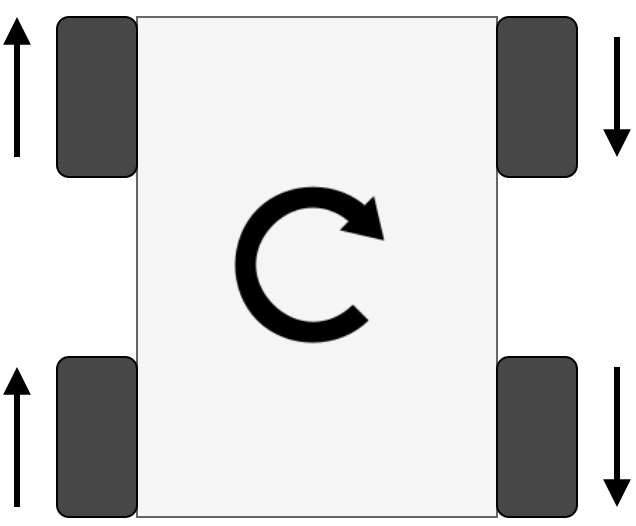
\includegraphics[width=0.4\linewidth]{informe_4/diagrama_giro.png}
\caption{Dirección de giro}
\end{figure}

\begin{enumerate}
\def\labelenumi{\arabic{enumi}.}
\setcounter{enumi}{2}
\item
  El sistema debe permitir el bloqueo de movimiento en una dirección
  (por ejemplo debido a un obstáulo detectado por el sensor de
  proximidad).

  Se cumplió parcialmente con el objetivo, ya que se puede bloquear solo
  el movimiento hacia adelante. Esto puede verse en el código:

\begin{lstlisting}
//bloquea el avance del vehiculo
void bloquear() {
   avance_bloqueado = TRUE;
}

...

void actualizar_desplazamiento() {

    switch (estado_auto) {

     //si el estado es adelante, todos los motores giran en un mismo sentido
     case ADELANTE:
         //El avance puede ser bloqueado por el detector de colisiones. En ese caso, se vuelve a actualizar el estado del vehiculo
         if (avance_bloqueado){
             estado_auto = FRENADO;
         }else{
             set_motor(M_DELANTERO_DER, M_MOV_ADELANTE, velocidad_avance);
             set_motor(M_DELANTERO_IZQ, M_MOV_ADELANTE, velocidad_avance);
             set_motor(M_TRASERO_DER, M_MOV_ADELANTE, velocidad_avance);
             set_motor(M_TRASERO_IZQ, M_MOV_ADELANTE, velocidad_avance);
         }
         break;

        ...
     }
\end{lstlisting}
\item
  OPT El sistema debe indicar mediante una serie de LEDs el estado de
  movimiento del vehículo.

No se cumplió con el objetivo opcional, ya que se buscó simplificar el
diseño del poncho.
\end{enumerate}

\paragraph{Control Remoto}

\begin{enumerate}
\def\labelenumi{\arabic{enumi}.}
\item
  El sistema debe establecer una conexión bluetooth con el sistema de
  control remoto.

  Se cumplió con el objetivo, utilizando un módulo Bluetooth HM-10
  provisto por la cátedra.
\item
  El sistema debe leer las indicaciones del control remoto y ejecutar
  las acciones correspondientes.

  Se cumplió con el objetivo, utilizando como control remoto una
  aplicación de celular, cuyo funcionamiento ya fue detallado con
  anterioridad.
\item
  El sistema debe indicar mediante un LED el estado de la conexión
  bluetooth.

  Se utilizó el LED que viene incluído en el módulo HM-10, que indica
  con una luz parpadeante si recibe alimentación, y una luz constante si
  se realizó la conexión.
\end{enumerate}

\paragraph{OPT Medición Sensores}

\begin{enumerate}
\def\labelenumi{\arabic{enumi}.}
\item
  Ante ausencia de luz externa, se deben encender las luces del vehículo

  No se cumplió con el objetivo, por demanda de tiempo y para
  simplificar el diseño del poncho.
\item
  Ante la presencia de obstáculos, se debe frenar el desplazamiento en
  esa dirección.

  Se cumplió con el objetivo, utilizando un sensor de proximidad
  ultrasónica, HC-SR04. Al utilizar un único sensor, con ángulo de
  visión de 15°, el vehículo solo frena el desplazamiento hacia
  adelante.
\end{enumerate}

\subsubsection{Requerimientos de Hardware}

\paragraph{Control de Motores}

\begin{enumerate}
\def\labelenumi{\arabic{enumi}.}
\item
  El vehículo debe utilizar puentes H para motores de corriente
  continua.

  Se cumplió con el objetivo, utilizando dos integrados L293D, dónde
  cada uno posee dos puentes H.
\item
  OPT El vehículo debe indicar con un LED para cada motor si este está
  en movimiento.

  No se cumplió con el objetivo, para simplificar el diseño del poncho.
\end{enumerate}

\paragraph{Baterías y cargador}

\begin{enumerate}
\def\labelenumi{\arabic{enumi}.}
\item
  El vehículo debe utilizar baterías de Litio para lograr la autonomía
  del vehículo

  Se cumplió con el objetivo, utilizando dos baterías de Litio en serie
  obteniendo una tensión de alimentación de aproximadamente 8V.
\item
  El vehículo debe indicar mediante un LED cuando haya baja tensión

  No se cumplió con el objetivo, no se pudo encontrar una manera
  sencilla de implementarlo.
\item
  El vehículo debe permitir cargar las baterías mediante un puerto USB.

  No se cumplió con el objetivo, ya que cargar el dispostivo con todos
  los componentes conectados podría generar problemas eléctricos.
\end{enumerate}

\paragraph{Componentes}

\begin{enumerate}
\def\labelenumi{\arabic{enumi}.}
\item
  Se debe contar con una llave de encendido/apagado y un LED que
  determine su estado.

  Se cumplió con el objetivo, se cuenta con una llave y varios LEDs que
  indican estado, ya que hay LEDs de alimentación en el Poncho, en la
  EDU-CIAA y en el módulo Bluetooth.
\item
  OPT El sistema debe poseer un buzzer para indicar eventos o fallas

  Se cumplió con el objetivo, el buzzer cumple dos funciones; notificar
  la presencia de obstáculos antes de bloquear el avance e indicar si el
  vehículo está retrocediendo.
\end{enumerate}

\subsection{Requerimientos No Funcionales}

\begin{itemize}
\tightlist
\item
  Utilizacion de la placa de desarrollo EDU-CIAA.
\item
  Estructura sólida y liviana, donde se colocan los motores y la
  EDU-CIAA.
\item
  El conexionado a los motores debe ser a través de borneras para poder
  cambiar la estructura.
\item
  Programación en lenguaje C.
\item
  Desarrollo de PCB en formato de poncho.
\item
  Mecanismo de control simple.
\item
  El sistema debe manejar respuestas en tiempo real.
\item
  Fecha de finalización y entrega del proyecto el día 16/12.
\end{itemize}

Se cumplieron todos los requerimientos no funcionales en tiempo y forma.

\subsection{Evaluación}

El grado de cumplimiento de los objetivos, en general, fue altamente
positivo. Los requerimientos funcionales que no se llevaron a cabo
fueron los de menor prioridad, la mayoría relacionados al hardware,
debido a que implicaban un costo de implementación muy alto para obtener
una funcionalidad muy reducida. Por ejemplo, el caso de colocar un led
que indique el estado de cada motor, lo cual costaría 4 pines GPIO, más
toda su interconexión, aumentando aún más la complejidad del poncho.

El principal cambio realizado fue el uso de una placa doble faz, por dos
motivos:

\begin{enumerate}
\def\labelenumi{\arabic{enumi}.}
\item
  Obtener un plano de tierra para disipar el calor producido por los
  integrados L293D.
\item
  Facilitar la conexión a tierra de los componentes, junto con el uso de
  puentes.
\end{enumerate}

Otro cambio fue el uso de una sola fuente step-down. En un principio la
alimentación iba a consistir de dos pilas de litio en paralelo, las
cuales entregarían aproximadamente 4v, y creíamos que sería necesario
utilizar dos conversores; un conversor step-up para alimentar los L293D
con 8v, y un conversor step-down para alimentar la EDU-CIAA con 3.3v.

Una vez estudiada mejor la arquitectura de la EDU-CIAA, observamos que
se alimentaba con 5v, y que internamente tiene un conversor a 3.3v para
aquellos puertos o componentes que necesiten de dicha tensión. Por este
motivo, cambiamos las pilas de paralelo a serie para obtener 8v que
alimentan directamente a los L293D, y utilizamos una fuente step-down
para alimentar la EDU-CIAA con 5v a través del conector Molex para
alimentación externa.

Un error que cometimos fue implementar mal la huella del conversor
step-down, la cual quedó completamente espejada, por lo que hubo que
colocarla sobre pines, y la tierra soldarla sobre el plano en lugar de
atravezando la placa.

\section{Actividad de los integrantes}

\begin{longtable}[]{@{}lll@{}}
\toprule
\begin{minipage}[b]{0.17\columnwidth}\raggedright
Tarea\strut
\end{minipage} & \begin{minipage}[b]{0.64\columnwidth}\raggedright
Descripción\strut
\end{minipage} & \begin{minipage}[b]{0.10\columnwidth}\raggedright
Tiempo\strut
\end{minipage}\tabularnewline
\midrule
\endhead
\begin{minipage}[t]{0.17\columnwidth}\raggedright
Compra de componentes\strut
\end{minipage} & \begin{minipage}[t]{0.64\columnwidth}\raggedright
Se obtuvieron los componentes electrónicos principales, los puentes H
(L293D) no se consiguieron individualmente por lo que se compró un
shield de Arduino que posee 2. Todos los componentes fueron comprados en
La Plata salvo las ruedas y motores. Componentes que requerían valores
precisos como resistencias y capacitores se fueron comprando a medida
que se concretaba el diseño.\strut
\end{minipage} & \begin{minipage}[t]{0.10\columnwidth}\raggedright
3 Horas\strut
\end{minipage}\tabularnewline
\begin{minipage}[t]{0.17\columnwidth}\raggedright
Estudio BT\strut
\end{minipage} & \begin{minipage}[t]{0.64\columnwidth}\raggedright
Mediante el uso de un módulo HM-10, el programa Hércules, la sAPI y un
aplicación para Android, se estudió el funcionamiento de la comunicación
Bluetooth. Se pudo concluir lo descripto en la sección de Software,
Bluetooth.\strut
\end{minipage} & \begin{minipage}[t]{0.10\columnwidth}\raggedright
8 Horas\strut
\end{minipage}\tabularnewline
\begin{minipage}[t]{0.17\columnwidth}\raggedright
Arquitectura de Software\strut
\end{minipage} & \begin{minipage}[t]{0.64\columnwidth}\raggedright
Se diseño la estructura principal del programa, como se describió en la
sección de software\strut
\end{minipage} & \begin{minipage}[t]{0.10\columnwidth}\raggedright
4 Horas\strut
\end{minipage}\tabularnewline
\begin{minipage}[t]{0.17\columnwidth}\raggedright
Estudio L293D\strut
\end{minipage} & \begin{minipage}[t]{0.64\columnwidth}\raggedright
Leyendo las datasheets del L293D y con recomendaciones de la cátedra, se
llegó a un diseño para la PCB que cumplía con los requisitos eléctricos
y térmicos. Además aquí también se incluye la investigación del módulo
PWM de la EDU-CIAA, para poder controlar la potencia de los
motores\strut
\end{minipage} & \begin{minipage}[t]{0.10\columnwidth}\raggedright
8 horas\strut
\end{minipage}\tabularnewline
\begin{minipage}[t]{0.17\columnwidth}\raggedright
Prototipo L293D\strut
\end{minipage} & \begin{minipage}[t]{0.64\columnwidth}\raggedright
Se utilizó un Arduino y el Shield mencionado para probar algunos motores
y el funcionamiento de los puentes H\strut
\end{minipage} & \begin{minipage}[t]{0.10\columnwidth}\raggedright
8 horas\strut
\end{minipage}\tabularnewline
\begin{minipage}[t]{0.17\columnwidth}\raggedright
Estudio de sensores\strut
\end{minipage} & \begin{minipage}[t]{0.64\columnwidth}\raggedright
Se investigó principalmente el funcionamiento del sensor de proximidad
HC-SR04\strut
\end{minipage} & \begin{minipage}[t]{0.10\columnwidth}\raggedright
4 horas\strut
\end{minipage}\tabularnewline
\begin{minipage}[t]{0.17\columnwidth}\raggedright
Estudio de batería\strut
\end{minipage} & \begin{minipage}[t]{0.64\columnwidth}\raggedright
Se vieron diferences opciones para la implementación de las baterías, la
caída de tensión en el L293D, tensión de las pilas de litio\strut
\end{minipage} & \begin{minipage}[t]{0.10\columnwidth}\raggedright
2 horas\strut
\end{minipage}\tabularnewline
\begin{minipage}[t]{0.17\columnwidth}\raggedright
Desarrollo de Software prioritario\strut
\end{minipage} & \begin{minipage}[t]{0.64\columnwidth}\raggedright
Se implementaron las partes más importantes del programa, el control de
motores y la comunicación Bluetooth\strut
\end{minipage} & \begin{minipage}[t]{0.10\columnwidth}\raggedright
8 horas\strut
\end{minipage}\tabularnewline
\begin{minipage}[t]{0.17\columnwidth}\raggedright
Estructura\strut
\end{minipage} & \begin{minipage}[t]{0.64\columnwidth}\raggedright
Se dejó para el final para centrarnos en la investigación y desarrollo
del poncho\strut
\end{minipage} & \begin{minipage}[t]{0.10\columnwidth}\raggedright
4 horas\strut
\end{minipage}\tabularnewline
\begin{minipage}[t]{0.17\columnwidth}\raggedright
Prototipo de Estructura\strut
\end{minipage} & \begin{minipage}[t]{0.64\columnwidth}\raggedright
El prototipo fue una precaria caja de zapatos, como se puede observar en
las fotos\strut
\end{minipage} & \begin{minipage}[t]{0.10\columnwidth}\raggedright
4 horas\strut
\end{minipage}\tabularnewline
\begin{minipage}[t]{0.17\columnwidth}\raggedright
Diseño de PCB\strut
\end{minipage} & \begin{minipage}[t]{0.64\columnwidth}\raggedright
El diseño de la PCB fue evolucionando constantemente, la estructura y
disposición de los componentes se mantuvo pero se fueron optimizando las
pistas.\strut
\end{minipage} & \begin{minipage}[t]{0.10\columnwidth}\raggedright
16 horas\strut
\end{minipage}\tabularnewline
\begin{minipage}[t]{0.17\columnwidth}\raggedright
Fabricación de PCB\strut
\end{minipage} & \begin{minipage}[t]{0.64\columnwidth}\raggedright
La PCB se fabricó en el ATEI con ayuda de Alejandro\strut
\end{minipage} & \begin{minipage}[t]{0.10\columnwidth}\raggedright
6 horas\strut
\end{minipage}\tabularnewline
\begin{minipage}[t]{0.17\columnwidth}\raggedright
Desarrollo de software secundario\strut
\end{minipage} & \begin{minipage}[t]{0.64\columnwidth}\raggedright
No se cumplió con el cronograma original, y se desarrollo los últimos
días\strut
\end{minipage} & \begin{minipage}[t]{0.10\columnwidth}\raggedright
6 horas\strut
\end{minipage}\tabularnewline
\begin{minipage}[t]{0.17\columnwidth}\raggedright
Montaje\strut
\end{minipage} & \begin{minipage}[t]{0.64\columnwidth}\raggedright
Se soldaron los componentes, se colocaron los motores, tornillos de
montaje, y porta pilas\strut
\end{minipage} & \begin{minipage}[t]{0.10\columnwidth}\raggedright
6 horas\strut
\end{minipage}\tabularnewline
\begin{minipage}[t]{0.17\columnwidth}\raggedright
Elección de baterías\strut
\end{minipage} & \begin{minipage}[t]{0.64\columnwidth}\raggedright
Dado el tamaño solo cabían dos pilas, las necesarias para llegar
8v.\strut
\end{minipage} & \begin{minipage}[t]{0.10\columnwidth}\raggedright
2 minutos\strut
\end{minipage}\tabularnewline
\begin{minipage}[t]{0.17\columnwidth}\raggedright
Calibración de Motores\strut
\end{minipage} & \begin{minipage}[t]{0.64\columnwidth}\raggedright
Se reguló la velocidad y se verificó que el mapeo de software coincida
con la implementación en hardware\strut
\end{minipage} & \begin{minipage}[t]{0.10\columnwidth}\raggedright
30 minutos\strut
\end{minipage}\tabularnewline
\begin{minipage}[t]{0.17\columnwidth}\raggedright
Validación\strut
\end{minipage} & \begin{minipage}[t]{0.64\columnwidth}\raggedright
Se verificó que el poncho y el software funciona correctamente y de
acuerdo a lo especificado. Hubo que reprogramar diveros sectores, como
el sensor de proximidad, que no actuaban acorde a lo especificado\strut
\end{minipage} & \begin{minipage}[t]{0.10\columnwidth}\raggedright
12 horas\strut
\end{minipage}\tabularnewline
\bottomrule
\end{longtable}

\section{Presupuesto}

\begin{longtable}[]{@{}ll@{}}
\toprule
Producto & Precio\tabularnewline
\midrule
\endhead
Shield motor driver arduino & \$ 350\tabularnewline
Ruedas con caja reductora y motores & \$ 1200\tabularnewline
Porta pilas de litio & \$ 150\tabularnewline
Placa virgen 10x15 doble faz & \$ 180\tabularnewline
Mini switch & \$ 45\tabularnewline
HC-SR04 & \$ 170\tabularnewline
Tira de 2x40 pines macho & \$ 80\tabularnewline
Step Down mini 360 & \$ 150\tabularnewline
Buzzer & \$ 30\tabularnewline
Resistencias/capacitores/leds/varios & \$ 200\tabularnewline
Transistor 2n7000 & \$ 20\tabularnewline
Hoja A4 papel fotográfico & \$ 20\tabularnewline
Horas de ingeniería (400hs.) & \$ 72000\tabularnewline
Total & \$ 74595\tabularnewline
\bottomrule
\end{longtable}

	
	% 8
	\chapter{Bibliografía}

\begin{enumerate}
	\item Hoja de datos del microcontrolador LPC4337 utilizado por la EDU-CIAA-NXP. Disponible en: \url{https://www.nxp.com/docs/en/data-sheet/LPC435X_3X_2X_1X.pdf}
	\item Hoja de datos de L293D. Disponible en: \url{http://www.ti.com/lit/ds/symlink/l293.pdf}
	
\end{enumerate}
	
	% 9
	\chapter{Anexo}

\section{Datasheets}

\begin{itemize}
	\item
	\textbf{Transistor 2n7000} Disponible:
	\url{https://www.onsemi.com/pub/Collateral/2N7000-D.PDF}
	\item
	\textbf{L293D Texas Instrument} Disponible:
	\url{http://www.ti.com/lit/ds/symlink/l293.pdf}
	\item
	\textbf{L293D STMicroelectronics} Disponible:
	\url{https://www.st.com/resource/en/datasheet/l293d.pdf}
	\item 
	\textbf{HC-SR04} \url{http://raspoid.com/download/datasheet/HCSR04}
	\item 
	\textbf{HC-SR04} \url{https://cdn.sparkfun.com/datasheets/Sensors/Proximity/HCSR04.pdf4}
	\item 
	\textbf{HC-SR04} \url{https://www.electroschematics.com/hc-sr04-datasheet/}
\end{itemize}

\section{Información general}

\begin{itemize}
	\item
	\textbf{HM-10} \url{https://github.com/ciaa/firmware\_v3/blob/master/examples/c/sapi/bluetooth/hm10\_uart\_bridge/EDU-CIAA-NXP\%20y\%20BLE\%204.0\%20HM10.pdf}
\end{itemize}

\section{Aplicaciones Externas}

\begin{itemize}
	\item
	\textbf{BLEJoystick} \url{https://play.google.com/store/apps/details?id=iyok.com.blejoystick}
\end{itemize}

\include{../informe_3/bom}

\section{Esquemático Completo}

	\section{Cronograma}


\begin{ganttchart}[vgrid, x unit = 0.9cm]{1}{12}
	\gantttitlelist{1,...,12}{1} \\
	\ganttbar[bar/.append style={fill=gray}]{Documentación}{1}{12} \\
	\ganttbar[bar/.append style={fill=gray}]{Compra Comp.}{1}{1} \\
	\ganttbar[bar/.append style={fill=gray}]{Estudio BT}{1}{2} \\
	\ganttbar[bar/.append style={fill=gray}]{Arq. SW}{2}{3} \\
	\ganttbar[bar/.append style={fill=gray}]{Estudio L293D}{2}{2} \\
	\ganttbar[bar/.append style={fill=gray}]{Proto. L293D}{3}{3} \\
	\ganttbar[bar/.append style={fill=gray}]{Estudio Sensores}{3}{3} \\
	\ganttbar[bar/.append style={fill=gray}]{Estudio Batería}{4}{4} \\
	\ganttbar[bar/.append style={fill=gray}]{SW Prioritario}{4}{5}{12} \\
	\ganttbar[bar/.append style={fill=gray}]{Estructura}{11}{12} \\
	\ganttbar[bar/.append style={fill=gray}]{Proto. estruct.}{11}{12} \\
	\ganttbar[bar/.append style={fill=gray}]{Diseño PCB}{8}{10} \\
	\ganttbar[bar/.append style={fill=gray}]{Fabr. PCB}{10}{10} \\
	\ganttbar[bar/.append style={fill=gray}]{SW Secundario}{11}{12} \\
	\ganttbar[bar/.append style={fill=gray}]{Montaje}{12}{12} \\
	\ganttbar[bar/.append style={fill=gray}]{Elección Bat.}{12}{12} \\
	\ganttbar[bar/.append style={fill=gray}]{Calibr. Motores}{12}{12} \\
	\ganttbar[bar/.append style={fill=gray}]{Validación}{11}{12}
	
\end{ganttchart}
\paragraph{}
Las unidades de tiempo son semanas. Consideramos dos semanas de Validación como margen en caso de eventualidades que atrasen el proyecto.

	\section{División de Tareas del Grupo}

\begin{tabular}{|c|c|}
	\hline 
	\textbf{Tarea a realizar} & \textbf{Alumno/s}  \\ 
	\hline 
	\sout{Obtención de electrónica} & \sout{Arreche, Blasco, Borini, Paradiso} \\ 
	\hline 
	\sout{Estudio de protocolos Bluetooth} & \sout{Arreche, Blasco, Borini, Paradiso} \\ 
	\hline 
	\sout{Arquitectura de software} & \sout{Arreche, Blasco, Borini, Paradiso} \\ 
	\hline 
	\sout{Estudio de L293D} & \sout{Arreche, Blasco, Borini, Paradiso} \\ 
	\hline 
	\sout{Prototipo L293D} & \sout{Arreche, Blasco, Borini, Paradiso} \\ 
	\hline 
	\sout{Investigación de sensores} & \sout{Arreche, Blasco, Borini, Paradiso} \\ 
	\hline 
	\sout{Investigación de baterías y carga} & \sout{Arreche, Blasco, Borini, Paradiso} \\ 
	\hline 
	\sout{Desarrollo de software prioritario} & \sout{Arreche, Blasco, Borini, Paradiso} \\ 
	\hline 
	\sout{Diseño} y fabricación de estructura & \sout{Arreche, Blasco, Borini, Paradiso} \\ 
	\hline 
	\sout{Proto. de estructura con motores y L293D} & \sout{Arreche, Blasco, Borini, Paradiso} \\ 
	\hline 
	\sout{Diseño de la PCB} & \sout{Arreche, Blasco, Borini, Paradiso} \\ 
	\hline 
	\sout{Fabricacion de PCB} & \sout{Arreche, Blasco, Borini, Paradiso} \\ 
	\hline 
	\sout{Desarrollo de SW secundario y sensores} & \sout{Arreche, Blasco, Borini, Paradiso} \\ 
	\hline 
	\sout{Montaje final} & \sout{Arreche, Blasco, Borini, Paradiso} \\ 
	\hline 
	\sout{Elección de baterías} & \sout{Arreche, Blasco, Borini, Paradiso} \\ 
	\hline 
	\sout{Calibración de motores} & \sout{Arreche, Blasco, Borini, Paradiso} \\ 
	\hline 
	\sout{Validación} & \sout{Arreche, Blasco, Borini, Paradiso} \\ 
	\hline 
	\sout{Documentación} & \sout{Arreche, Blasco, Borini, Paradiso} \\ 
	\hline 
\end{tabular} 
	\section{Manual de Usuario}

\begin{enumerate}
\def\labelenumi{\arabic{enumi}.}
\item
  Para poder utilizar el vehículo, se debe tener la aplicación BLE
  Joystick instalada en un teléfono Android.
  
\url{https://play.google.com/store/apps/details?id=iyok.com.blejoystick}
\item
  El vehículo contiene una llave para cortar la alimentación de
  baterías:
\end{enumerate}

\begin{figure}[H]
\centering
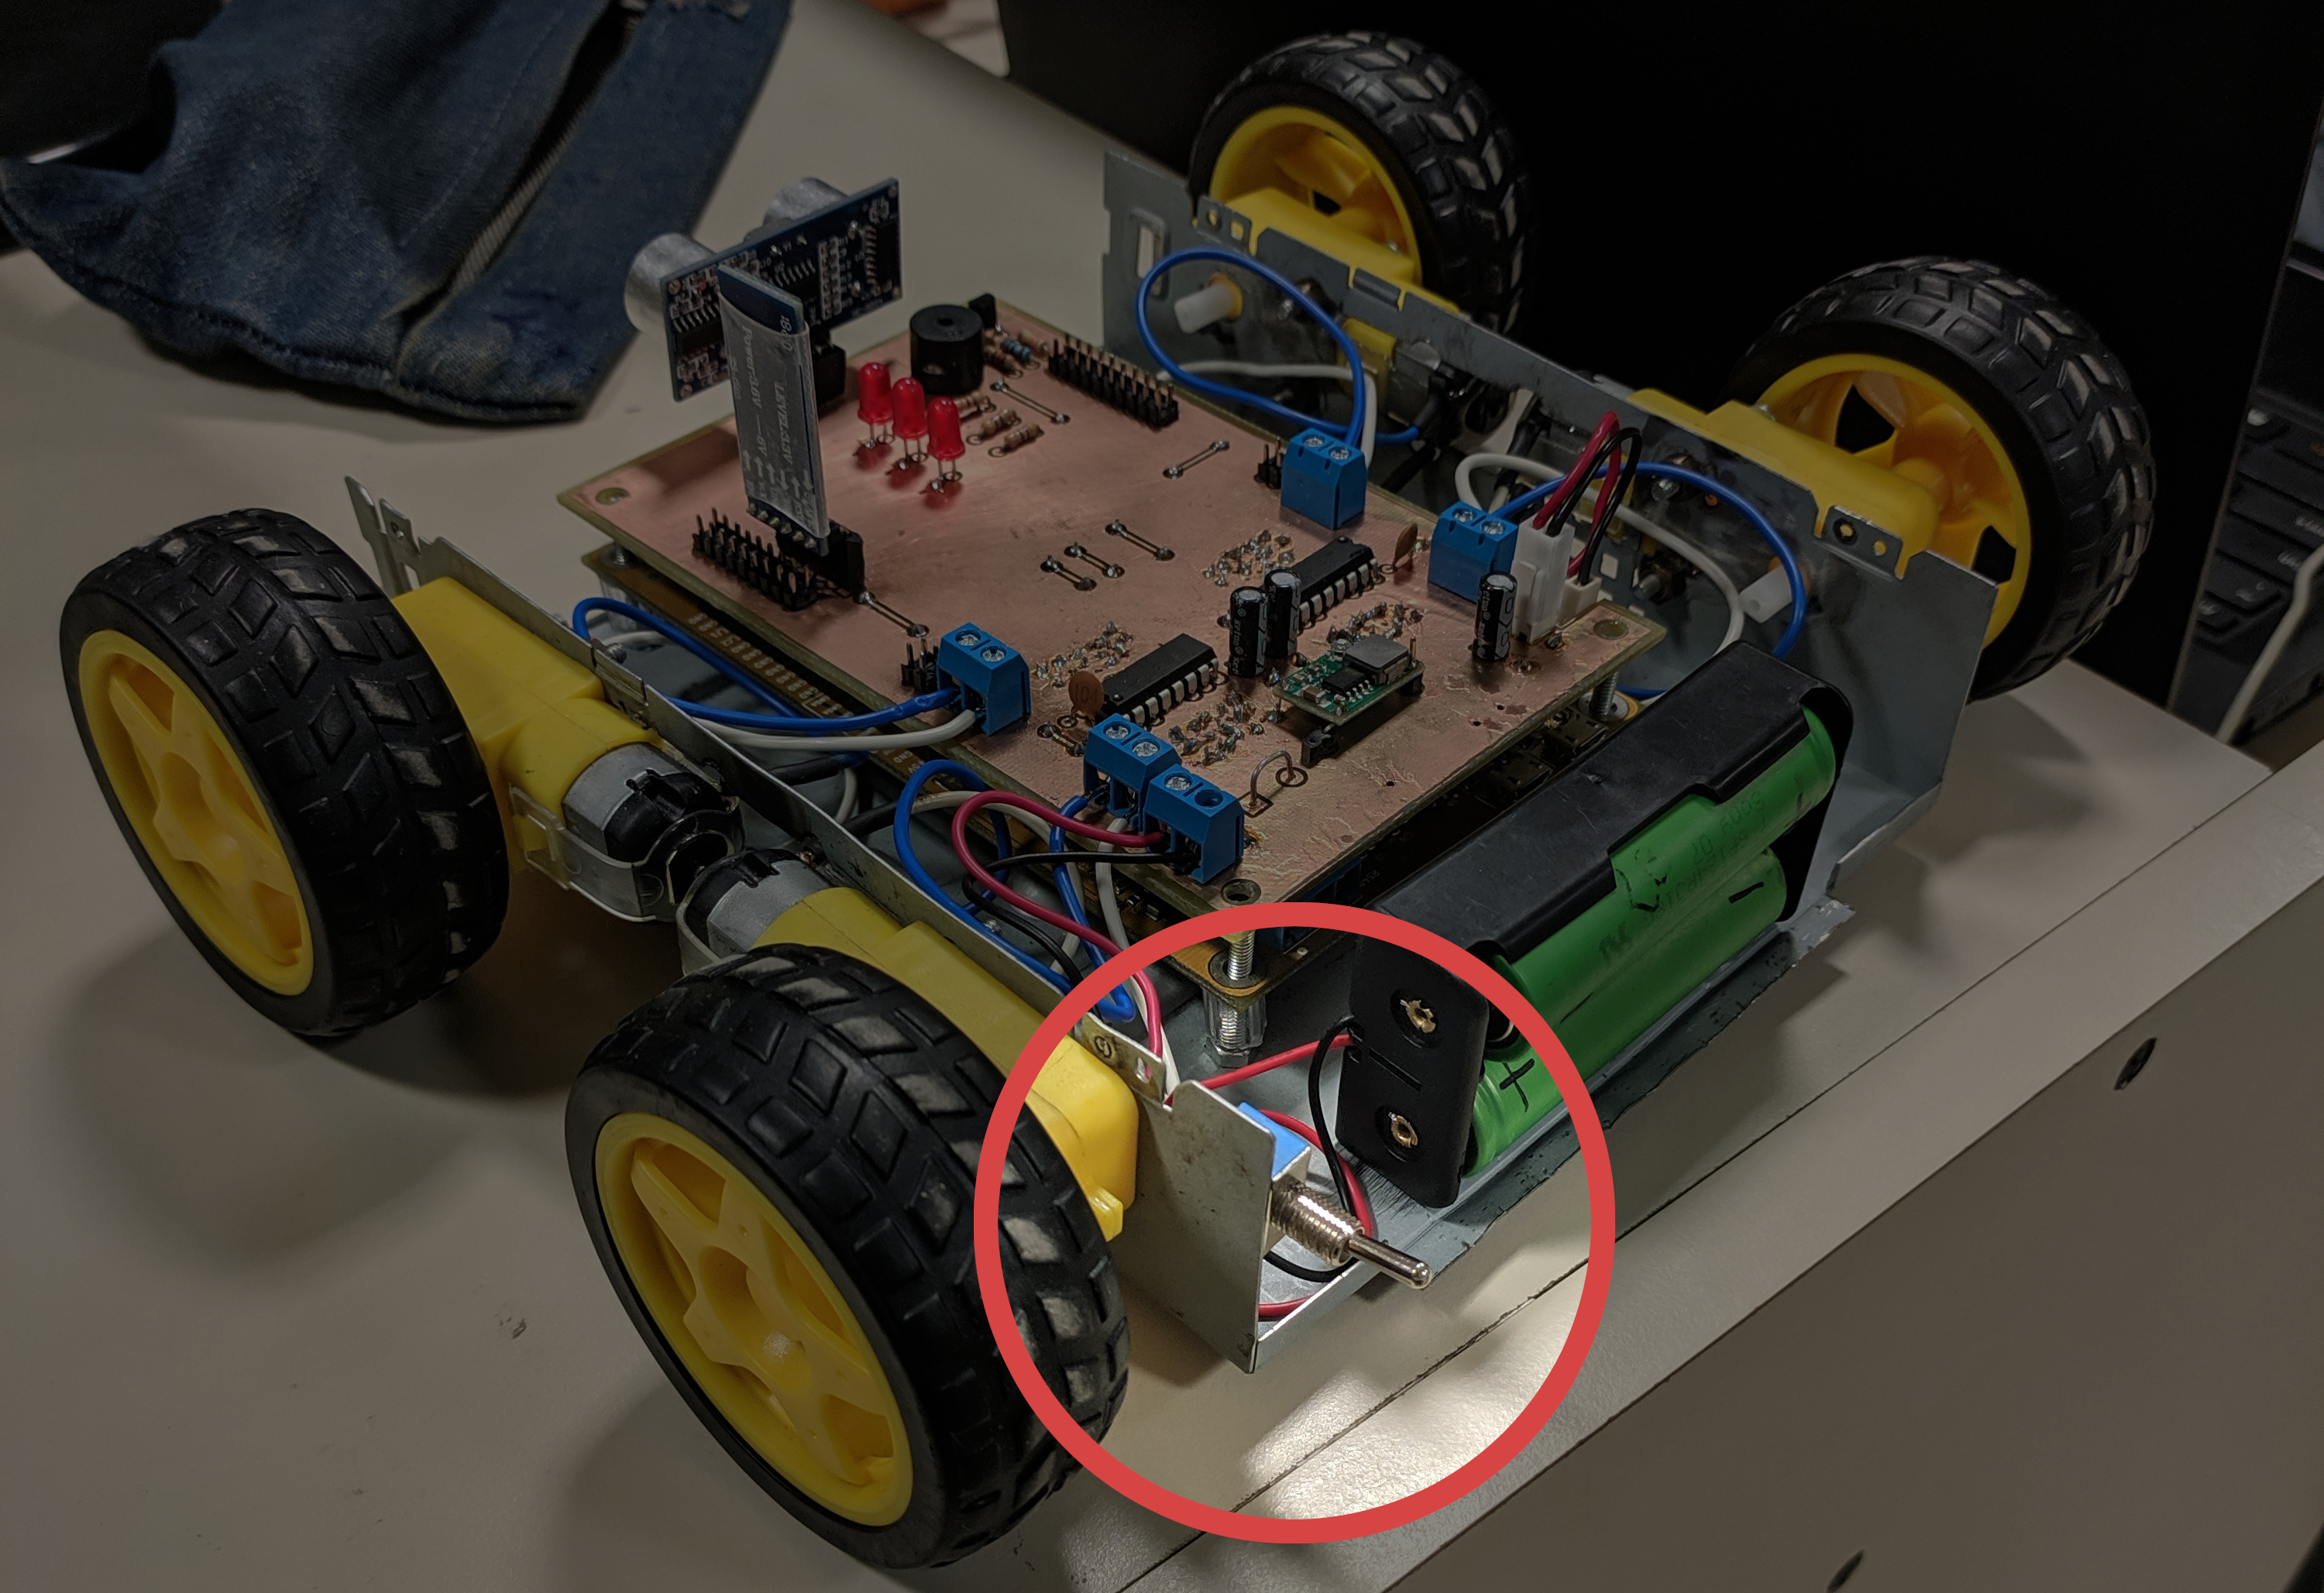
\includegraphics[width=0.8\linewidth]{informe_4/llave.jpg}
\caption{Llave de encendido}
\end{figure}

\begin{enumerate}
\def\labelenumi{\arabic{enumi}.}
\setcounter{enumi}{2}
\tightlist
\item
Conectar el teléfono al módulo Bluetooth del vehículo, una vez establecida la conexión, el LED del módulo HM-10 quedará fijo y dejará de titilar.
\end{enumerate}

	
	% 10
	\section{Imágenes del Proyecto}

\subsection{Desarrollo}

\begin{figure}[H]
	\centering
	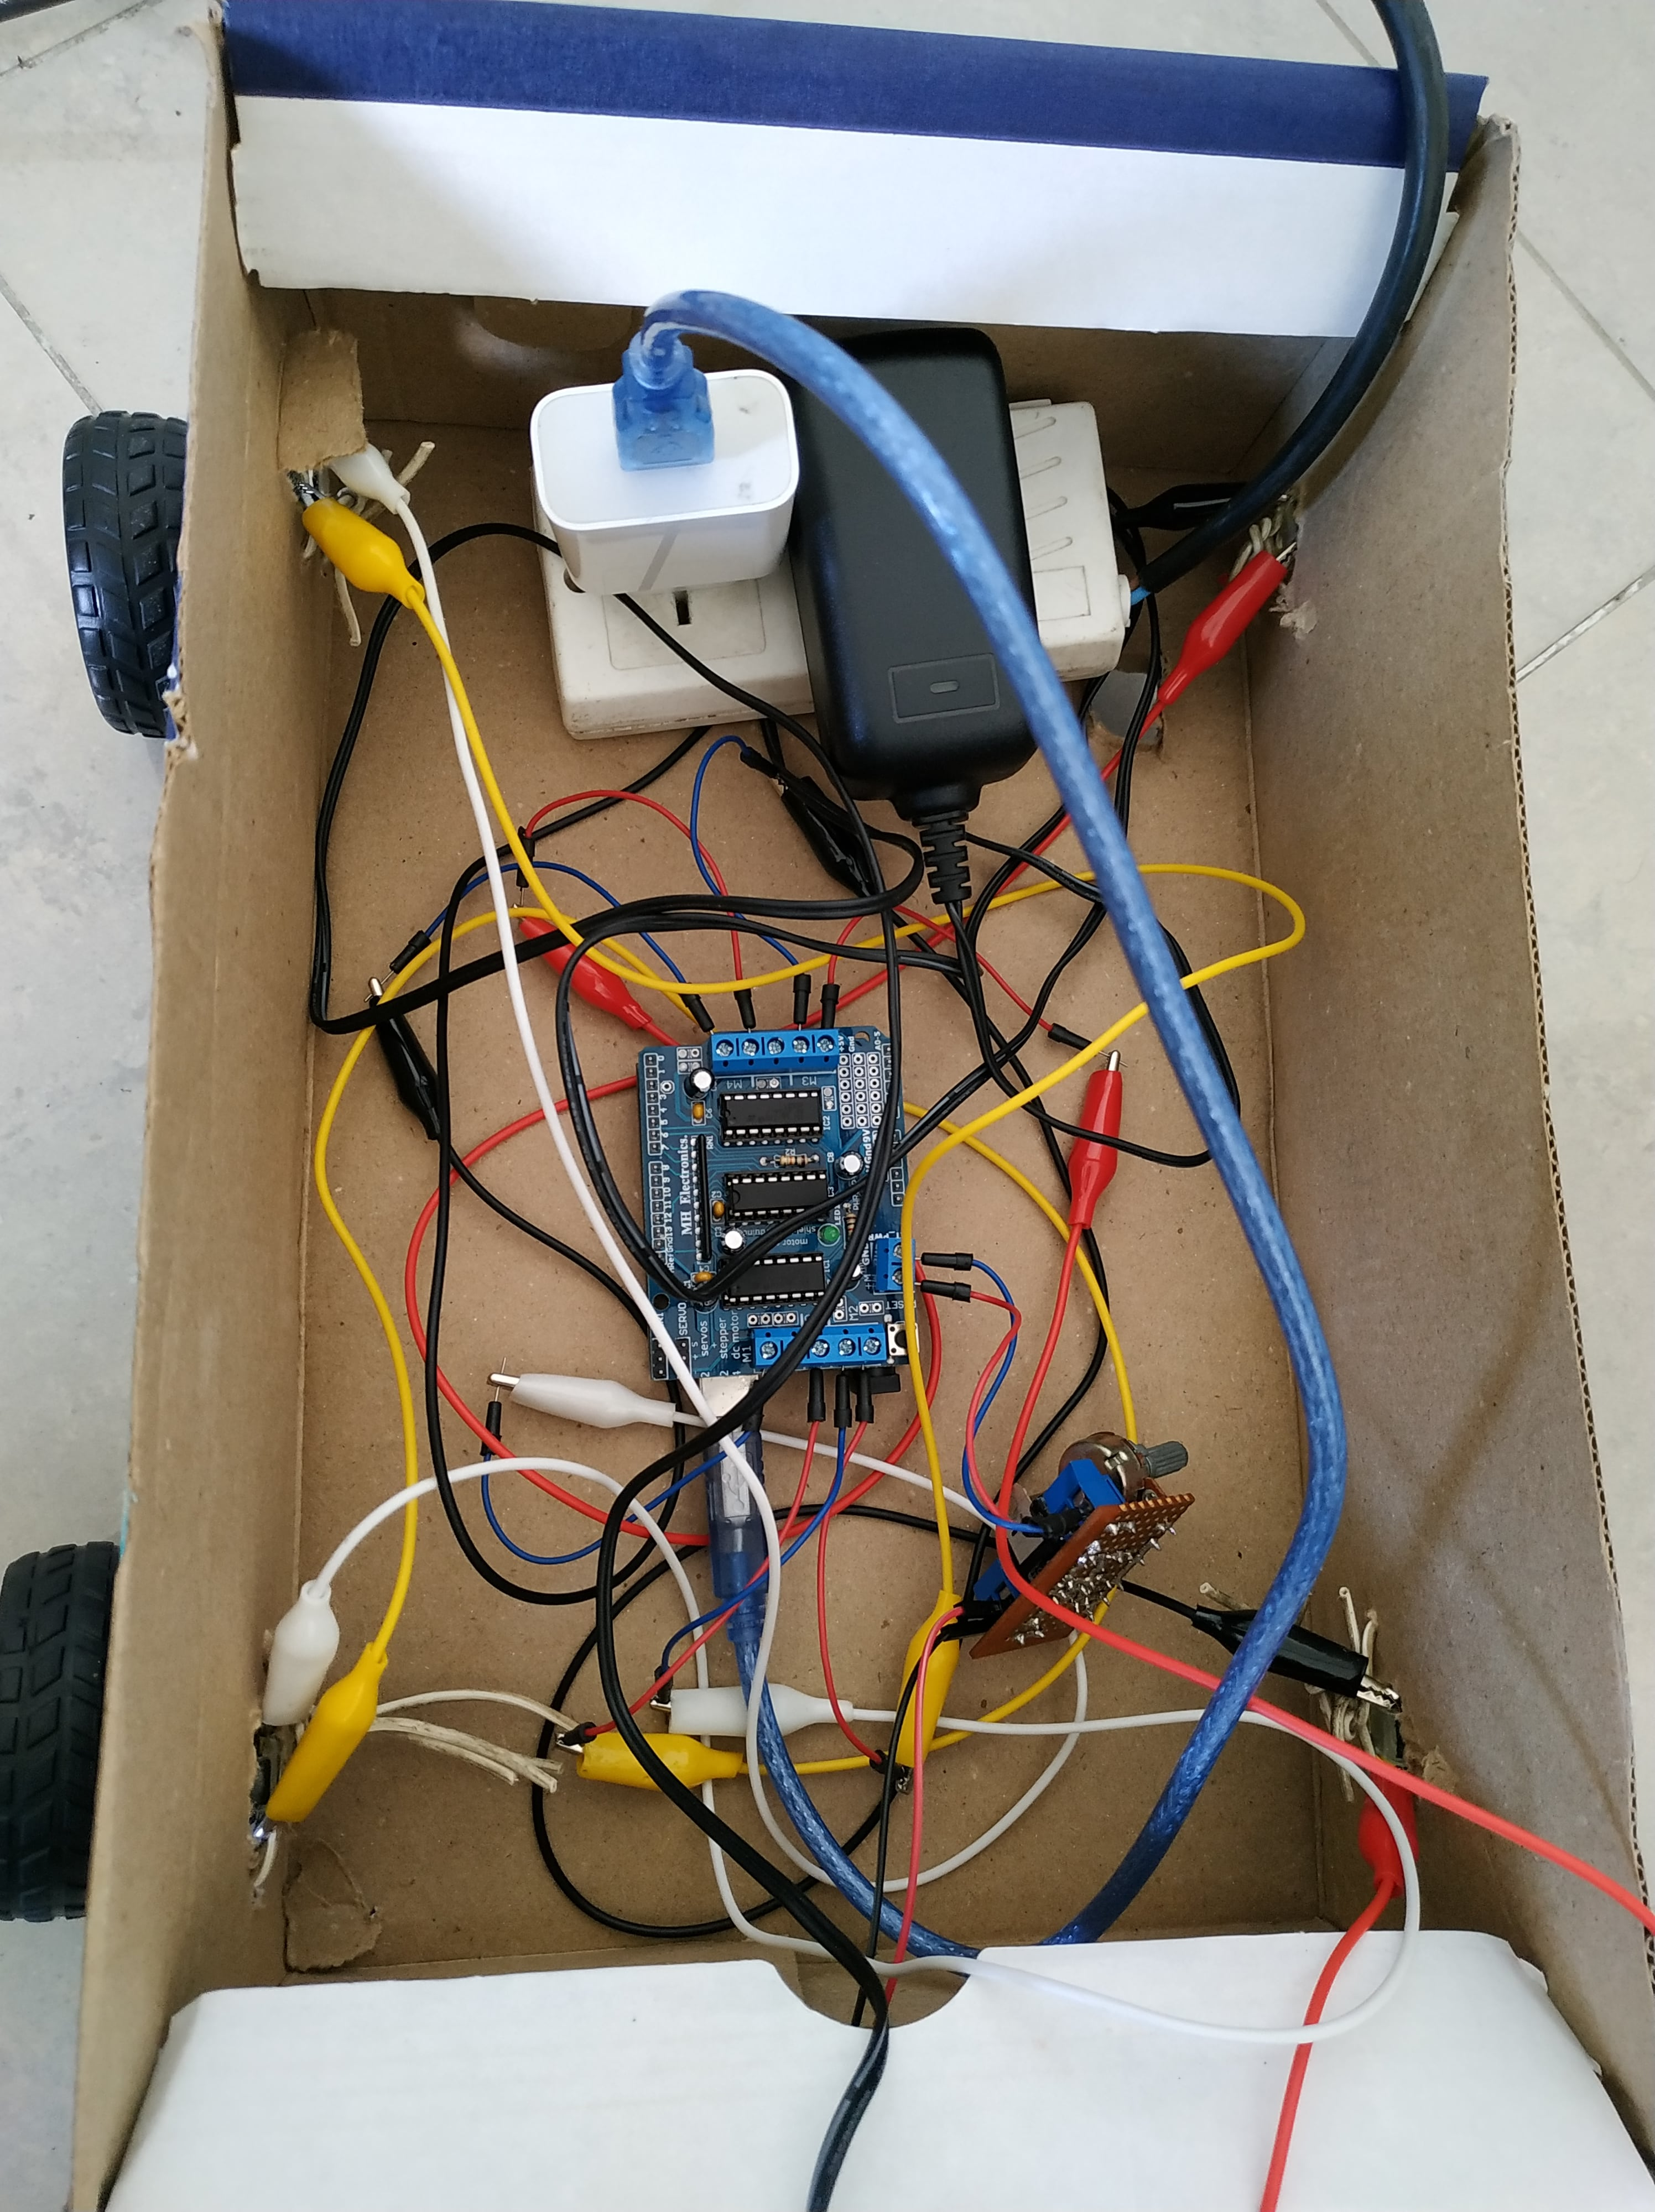
\includegraphics[width=0.9\linewidth]{imagenes/ensayo1.jpg}
	\caption{Prototipo utilizando Arduino}
	\label{fig:ensayo1}
\end{figure}

\begin{figure}[H]
	\centering
	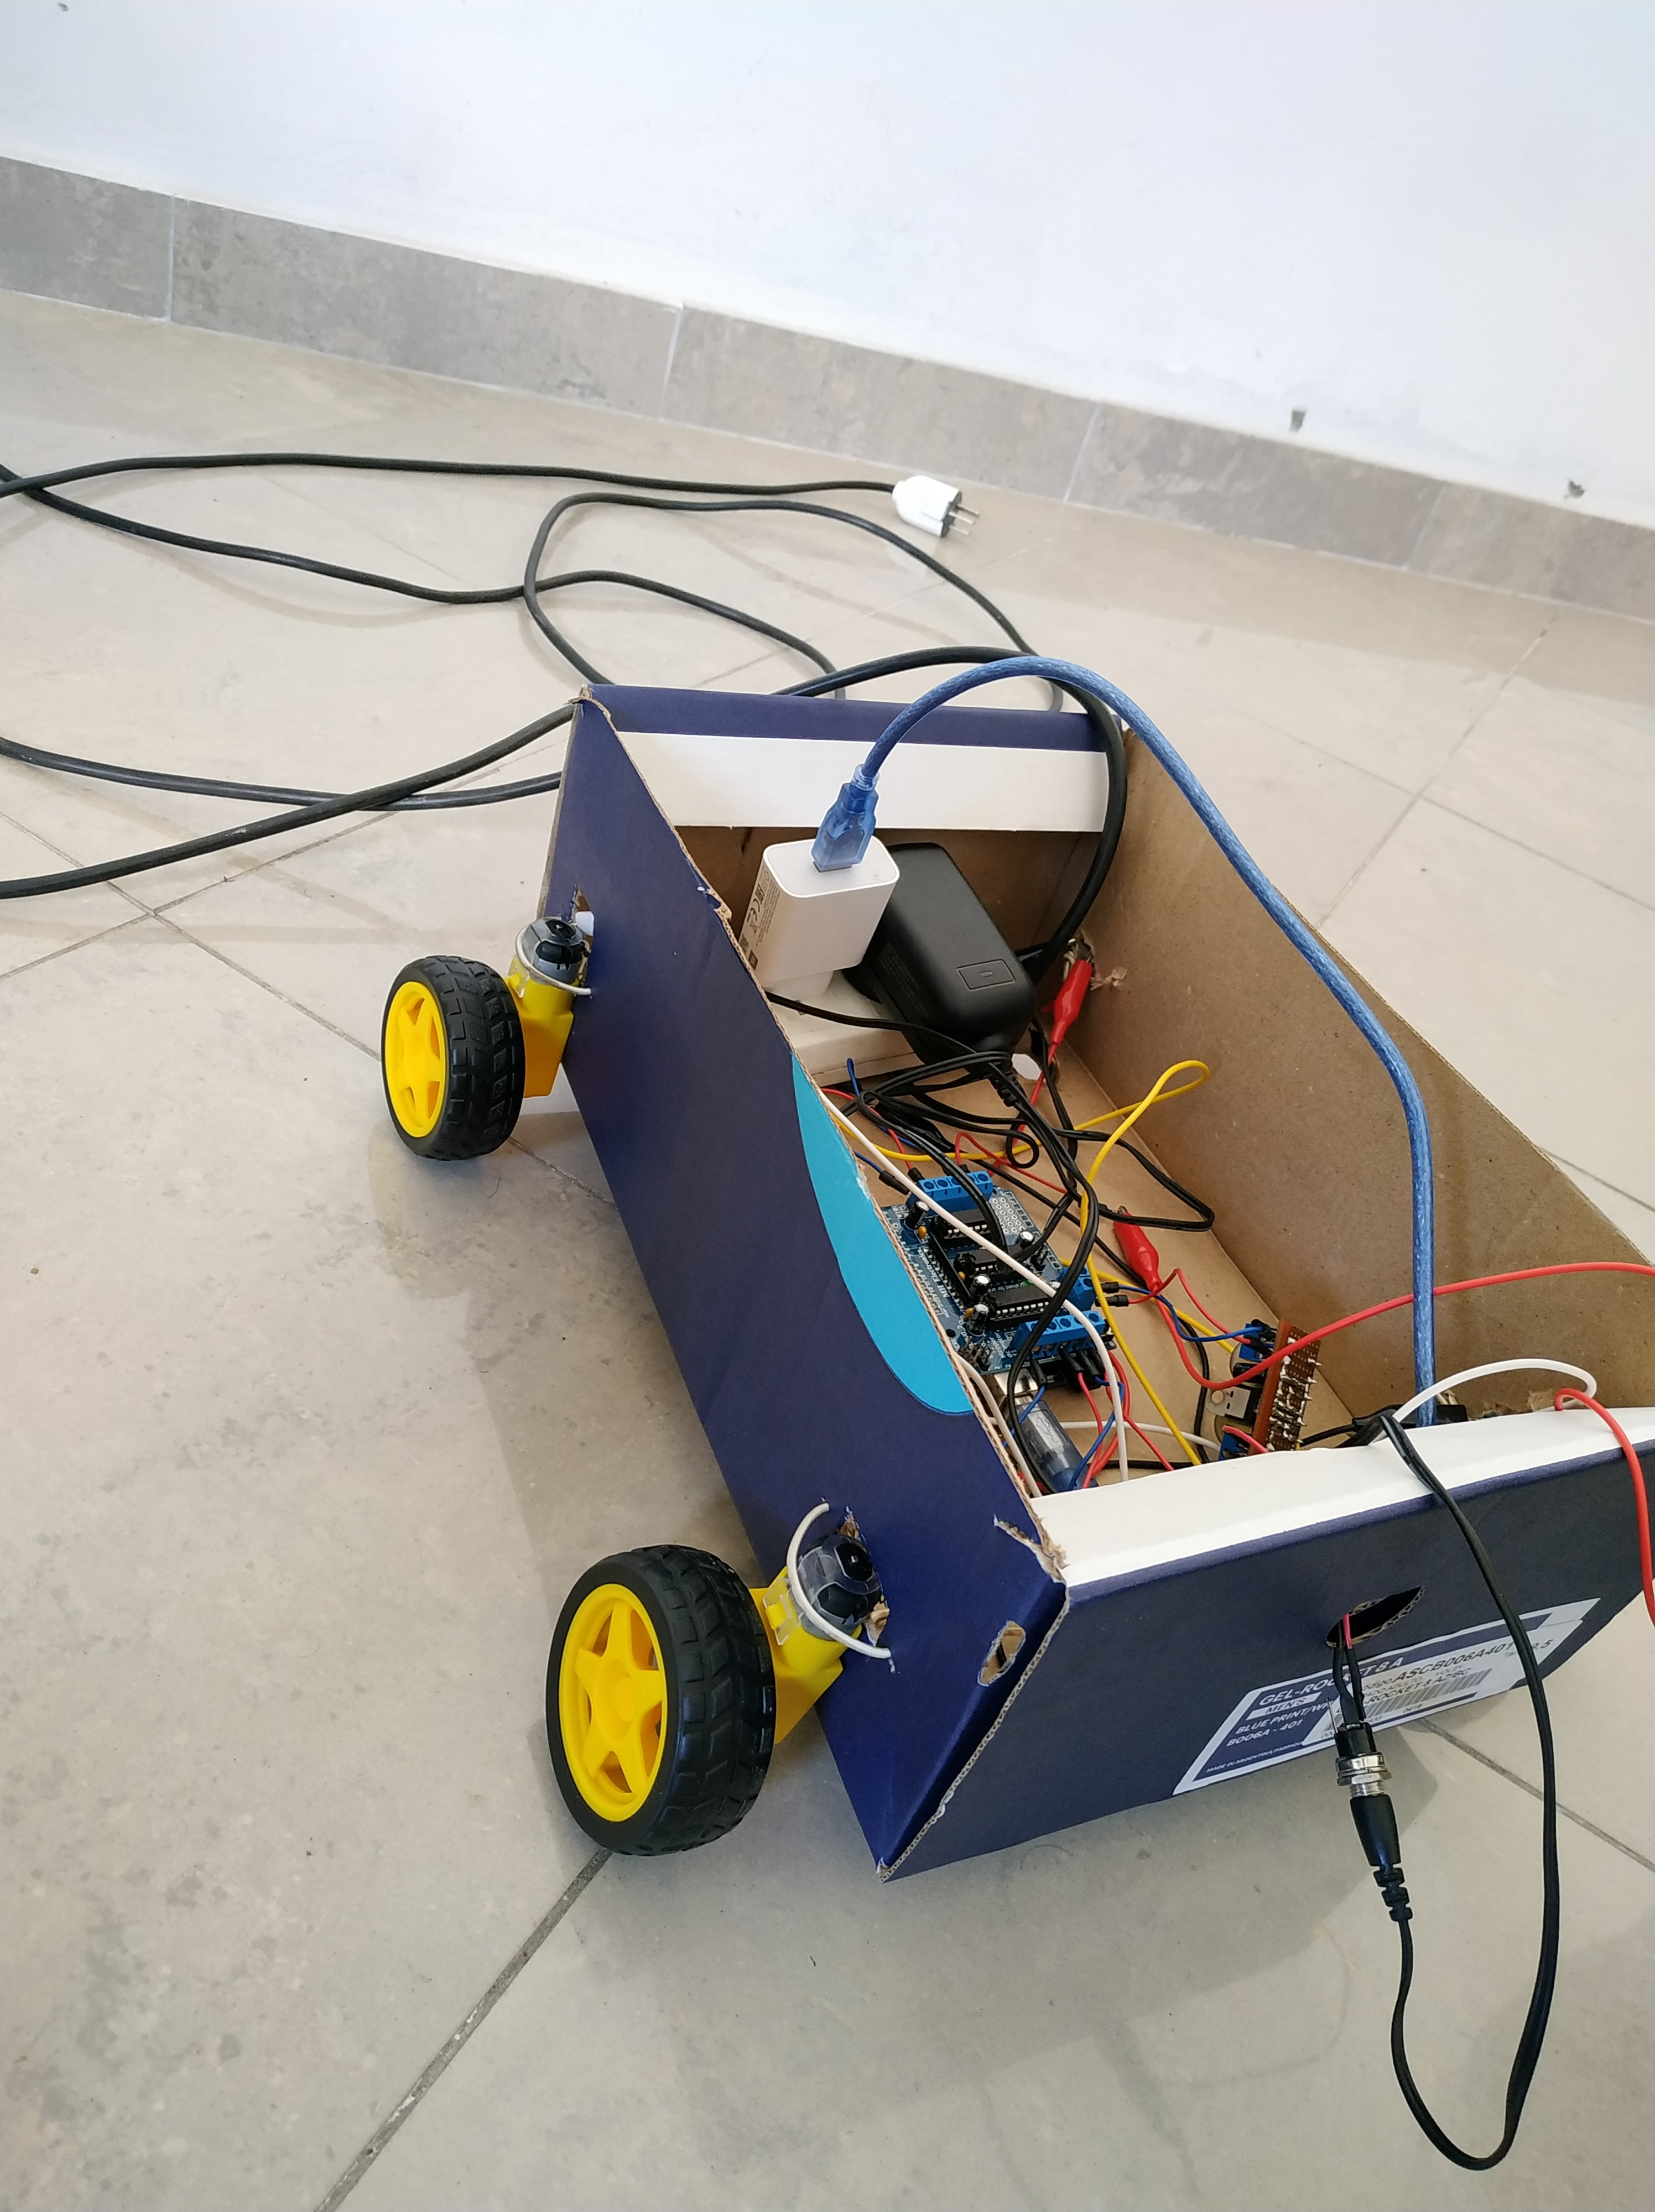
\includegraphics[width=0.9\linewidth]{imagenes/ensayo2.jpg}
	\caption{Prototipo utilizando Arduino}
	\label{fig:ensayo2}
\end{figure}

\begin{figure}[H]
\centering
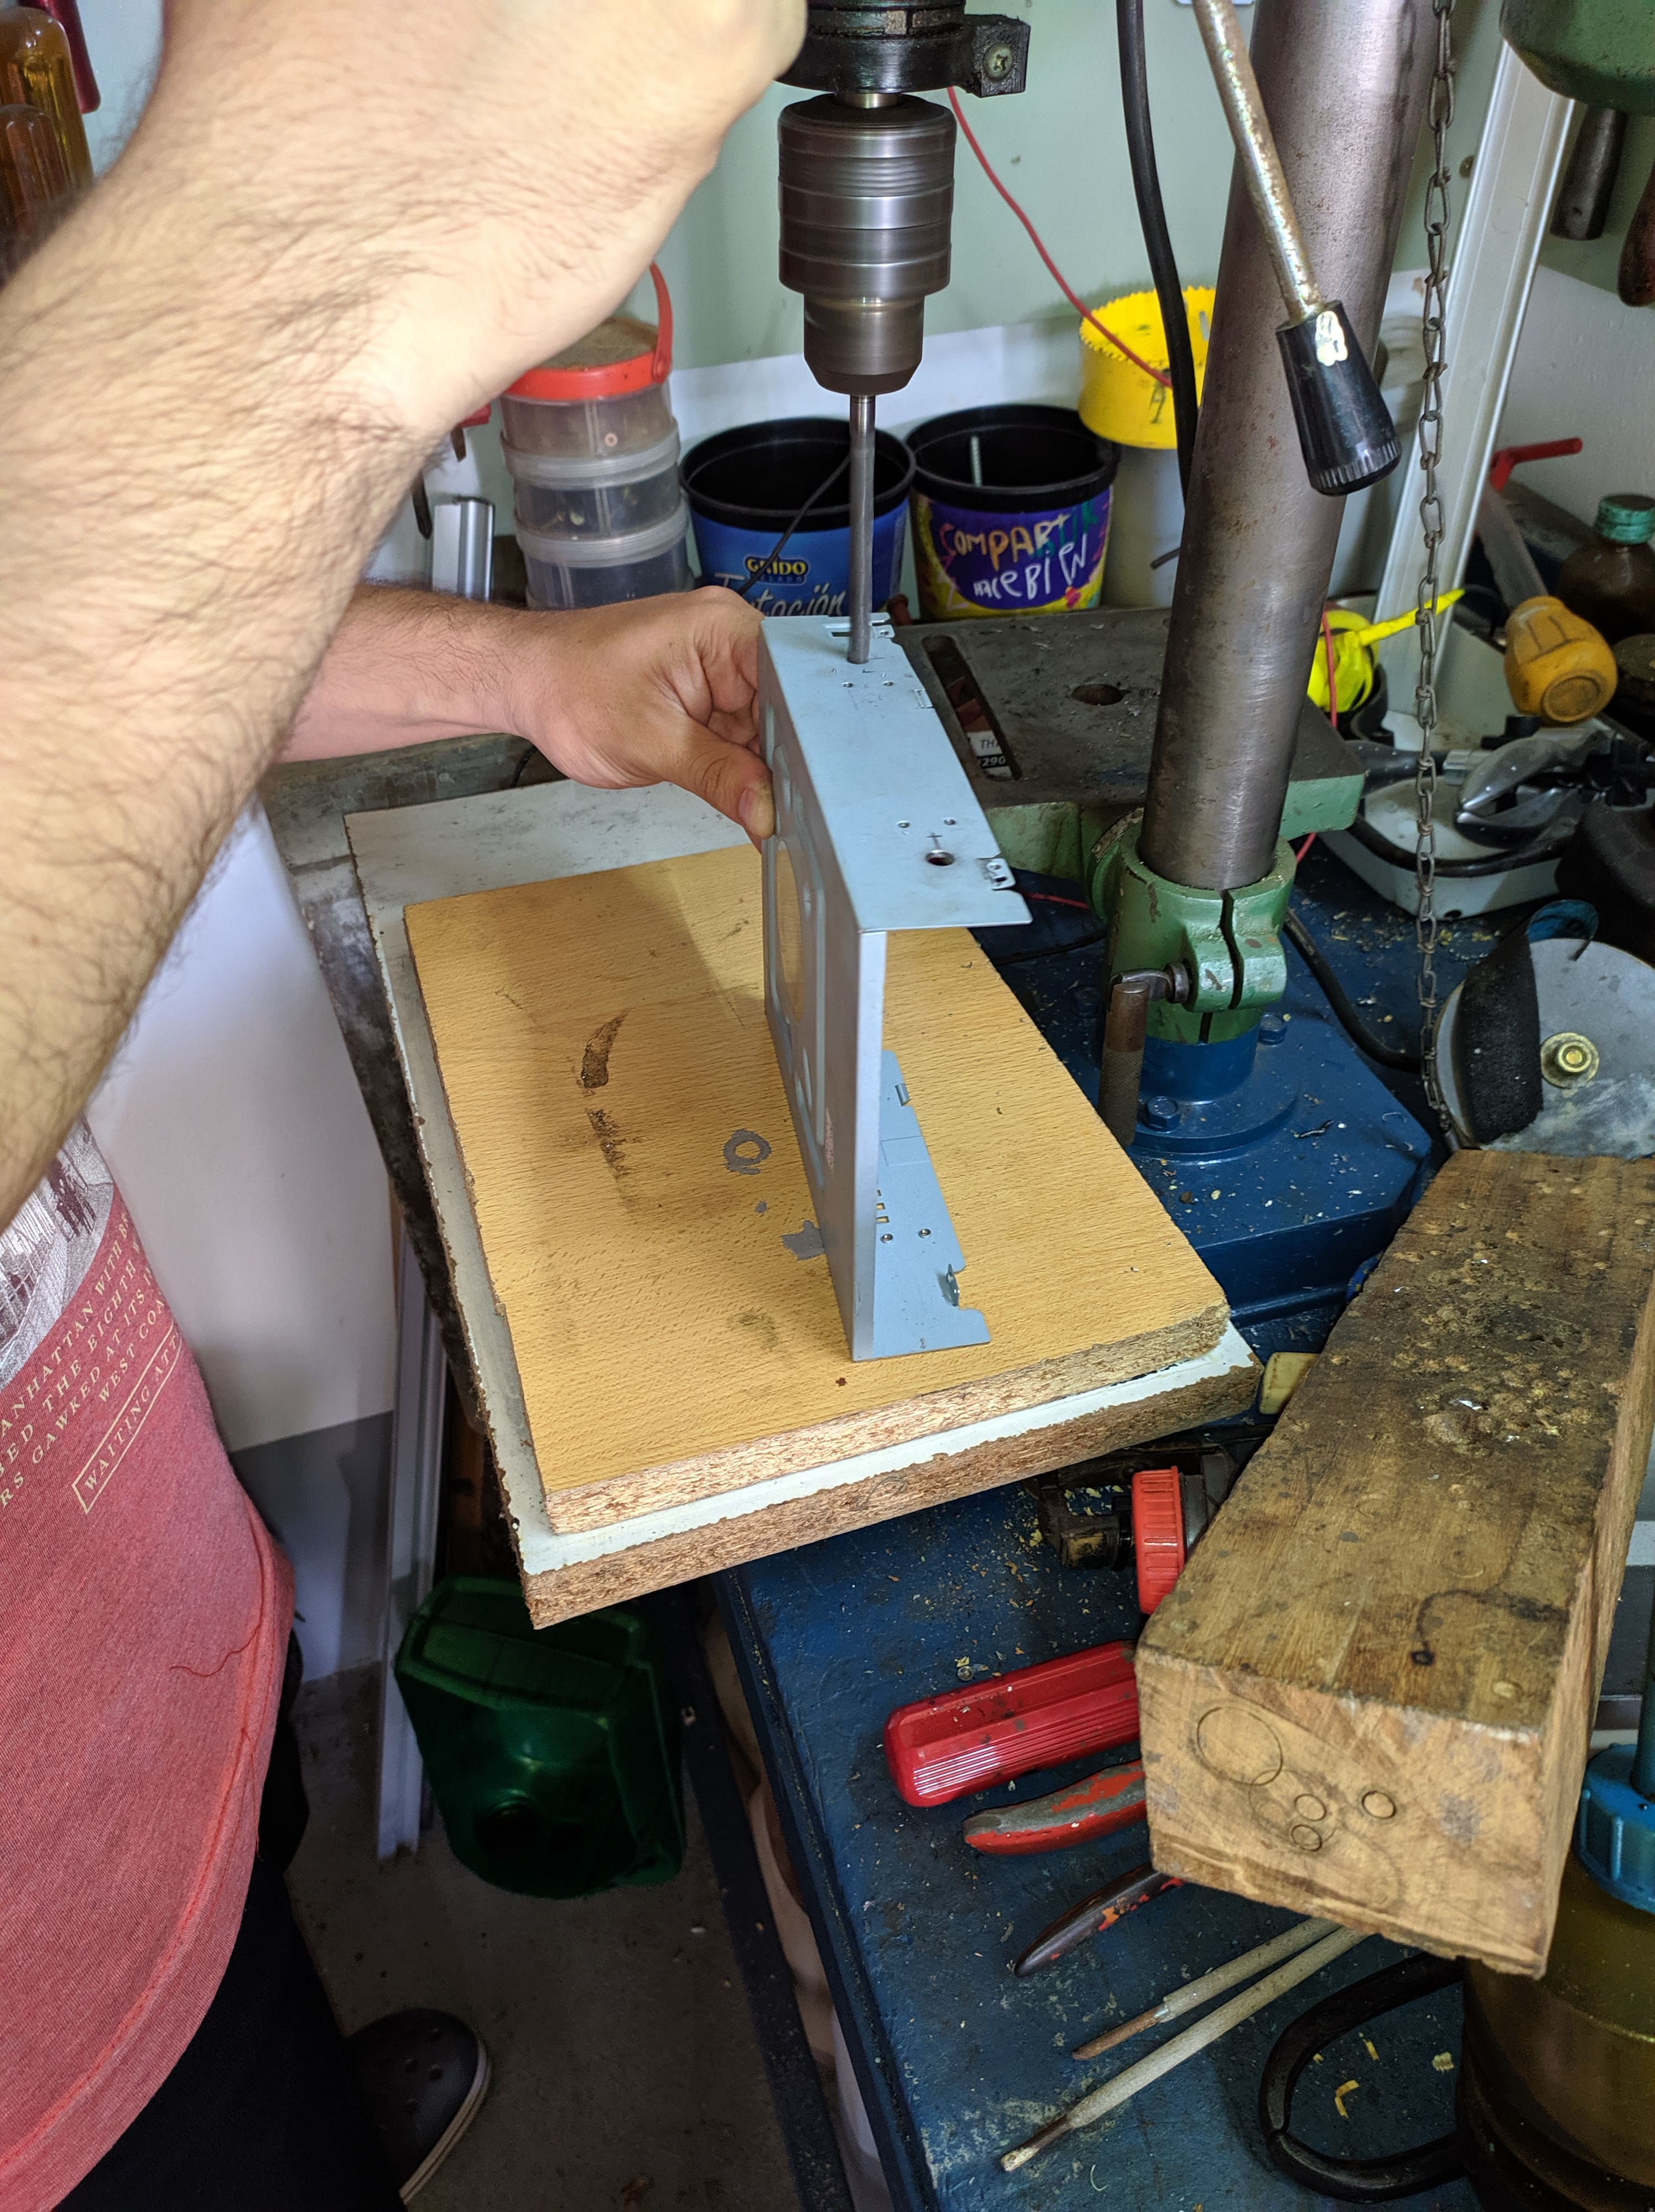
\includegraphics[width=0.9\linewidth]{imagenes/carcasa1.jpg}
\caption{Fabricación de la estructura}
\label{fig:agujero-caja}
\end{figure}

\begin{figure}[H]
	\centering
	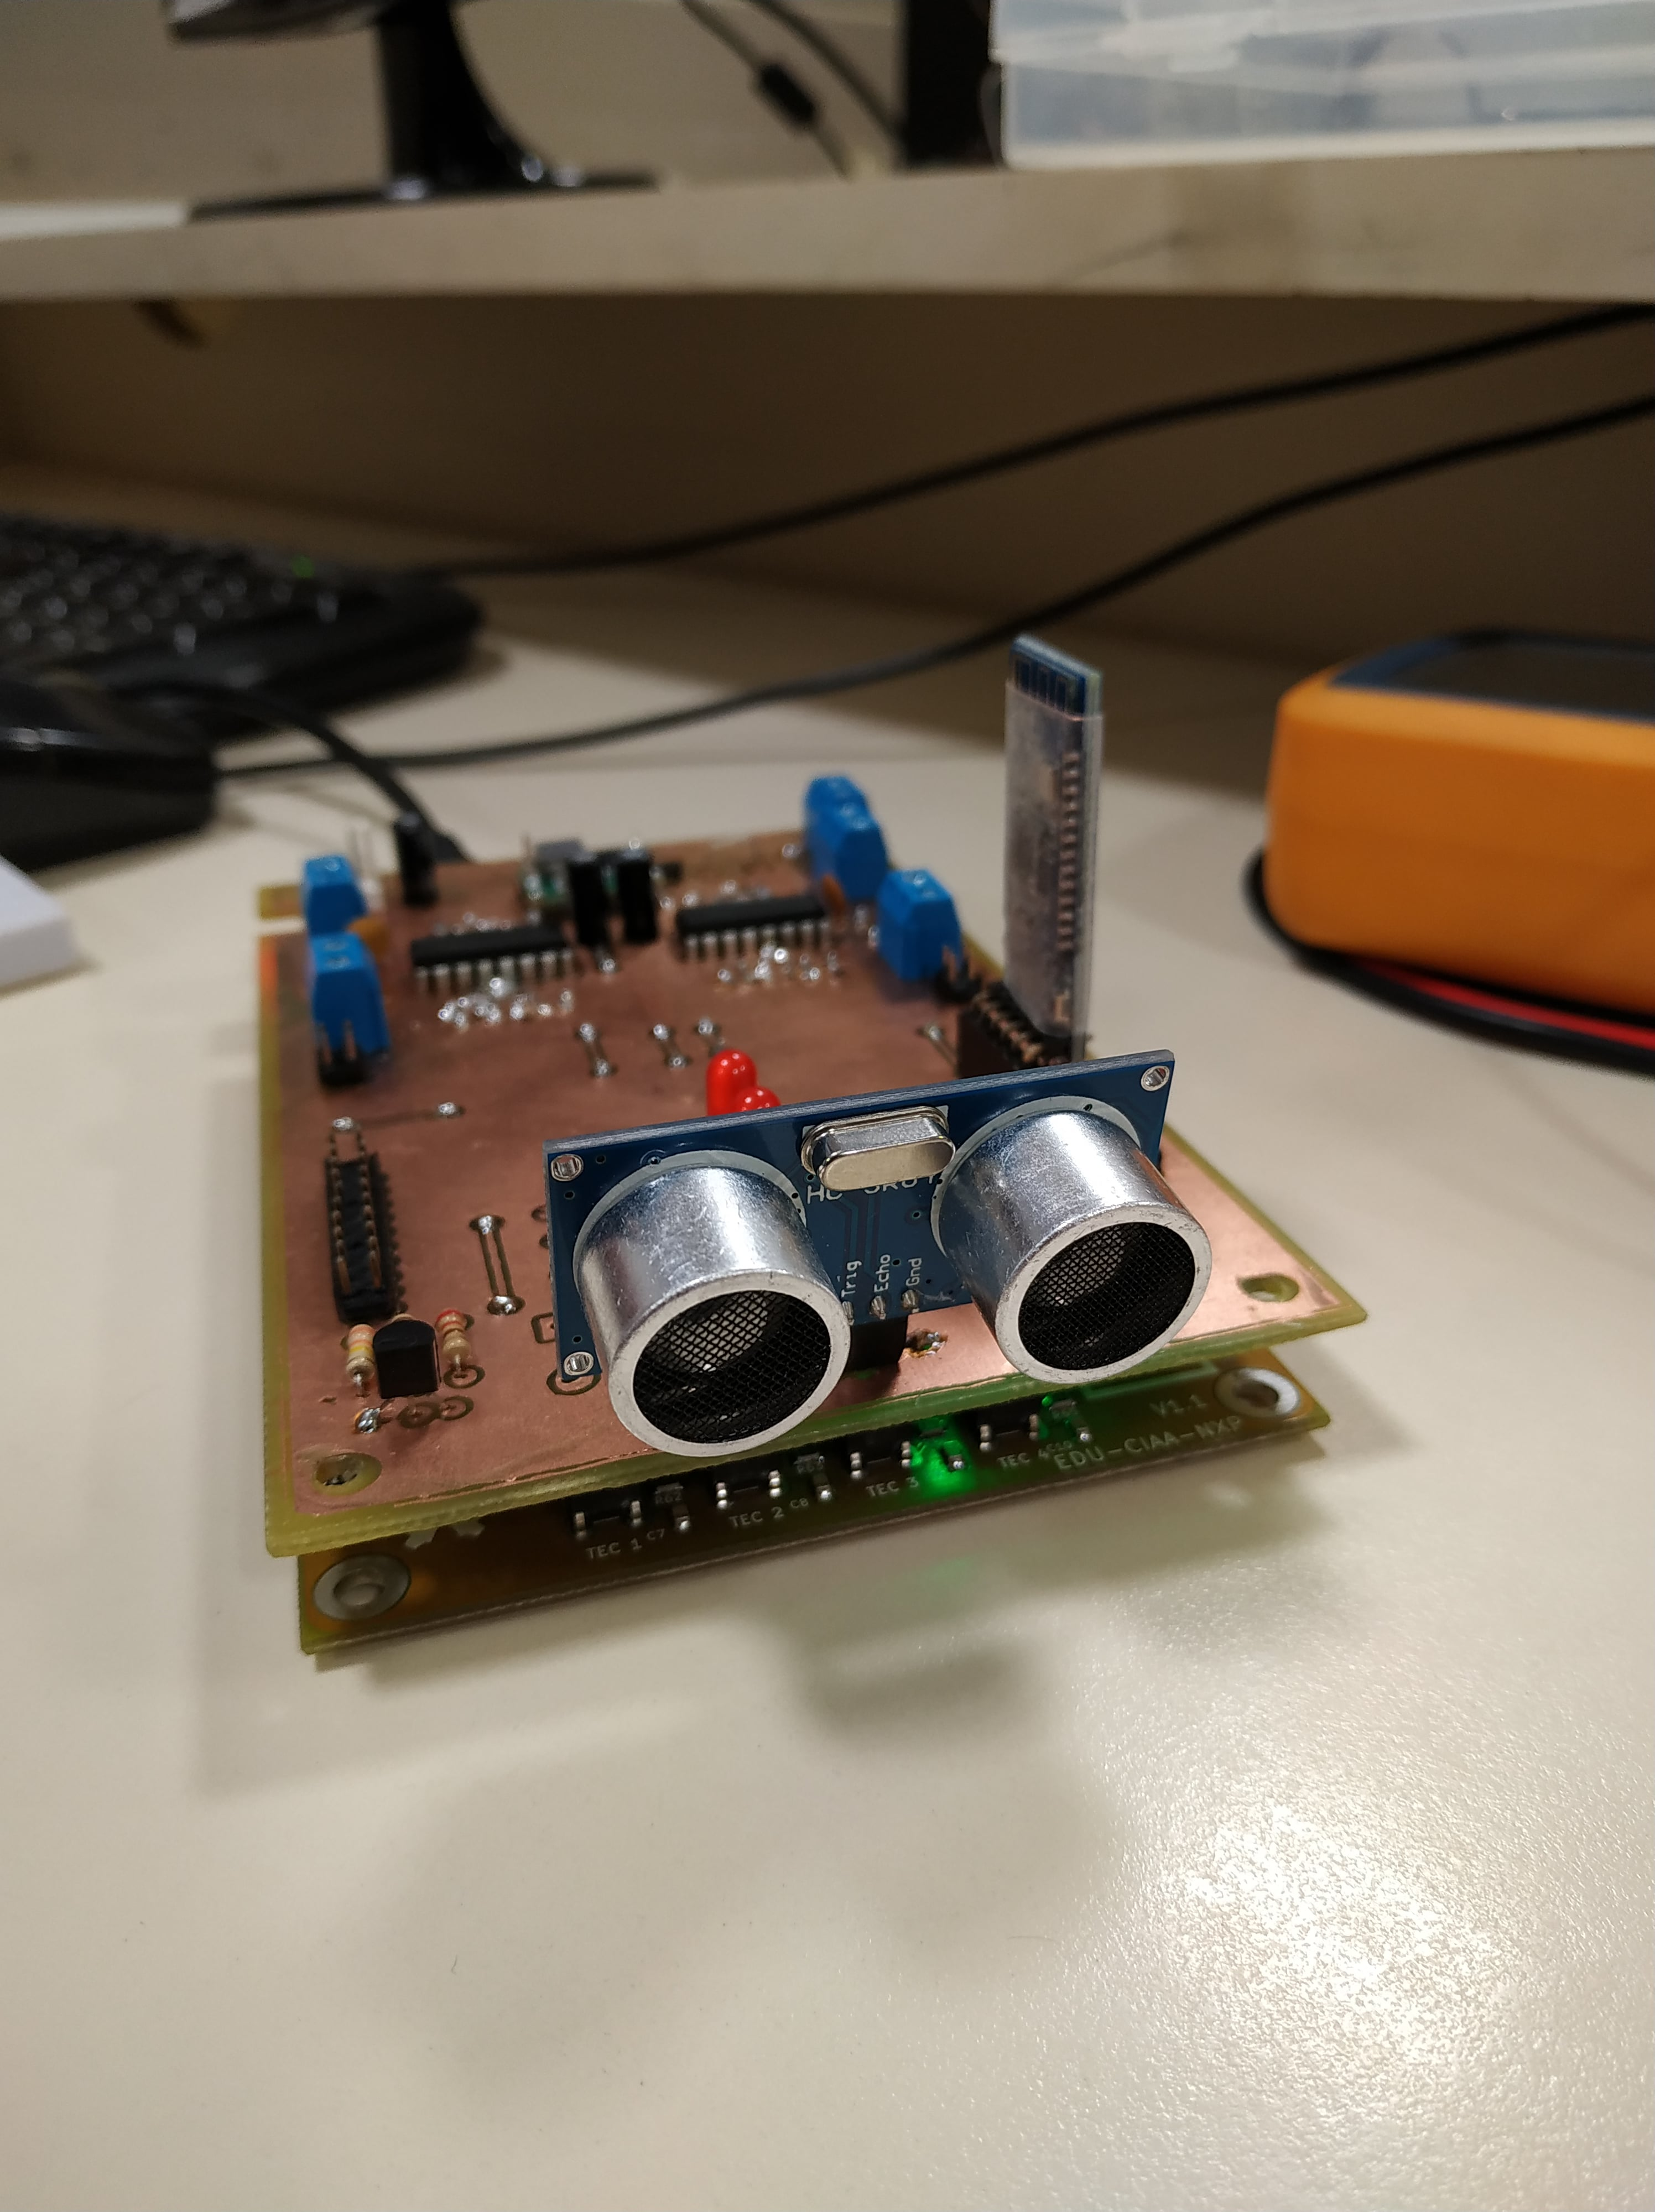
\includegraphics[width=0.9\linewidth]{imagenes/pruebas_software.jpg}
	\caption{Pruebas de software}
	\label{fig:prueba-software}
\end{figure}

\begin{figure}[H]
	\centering
	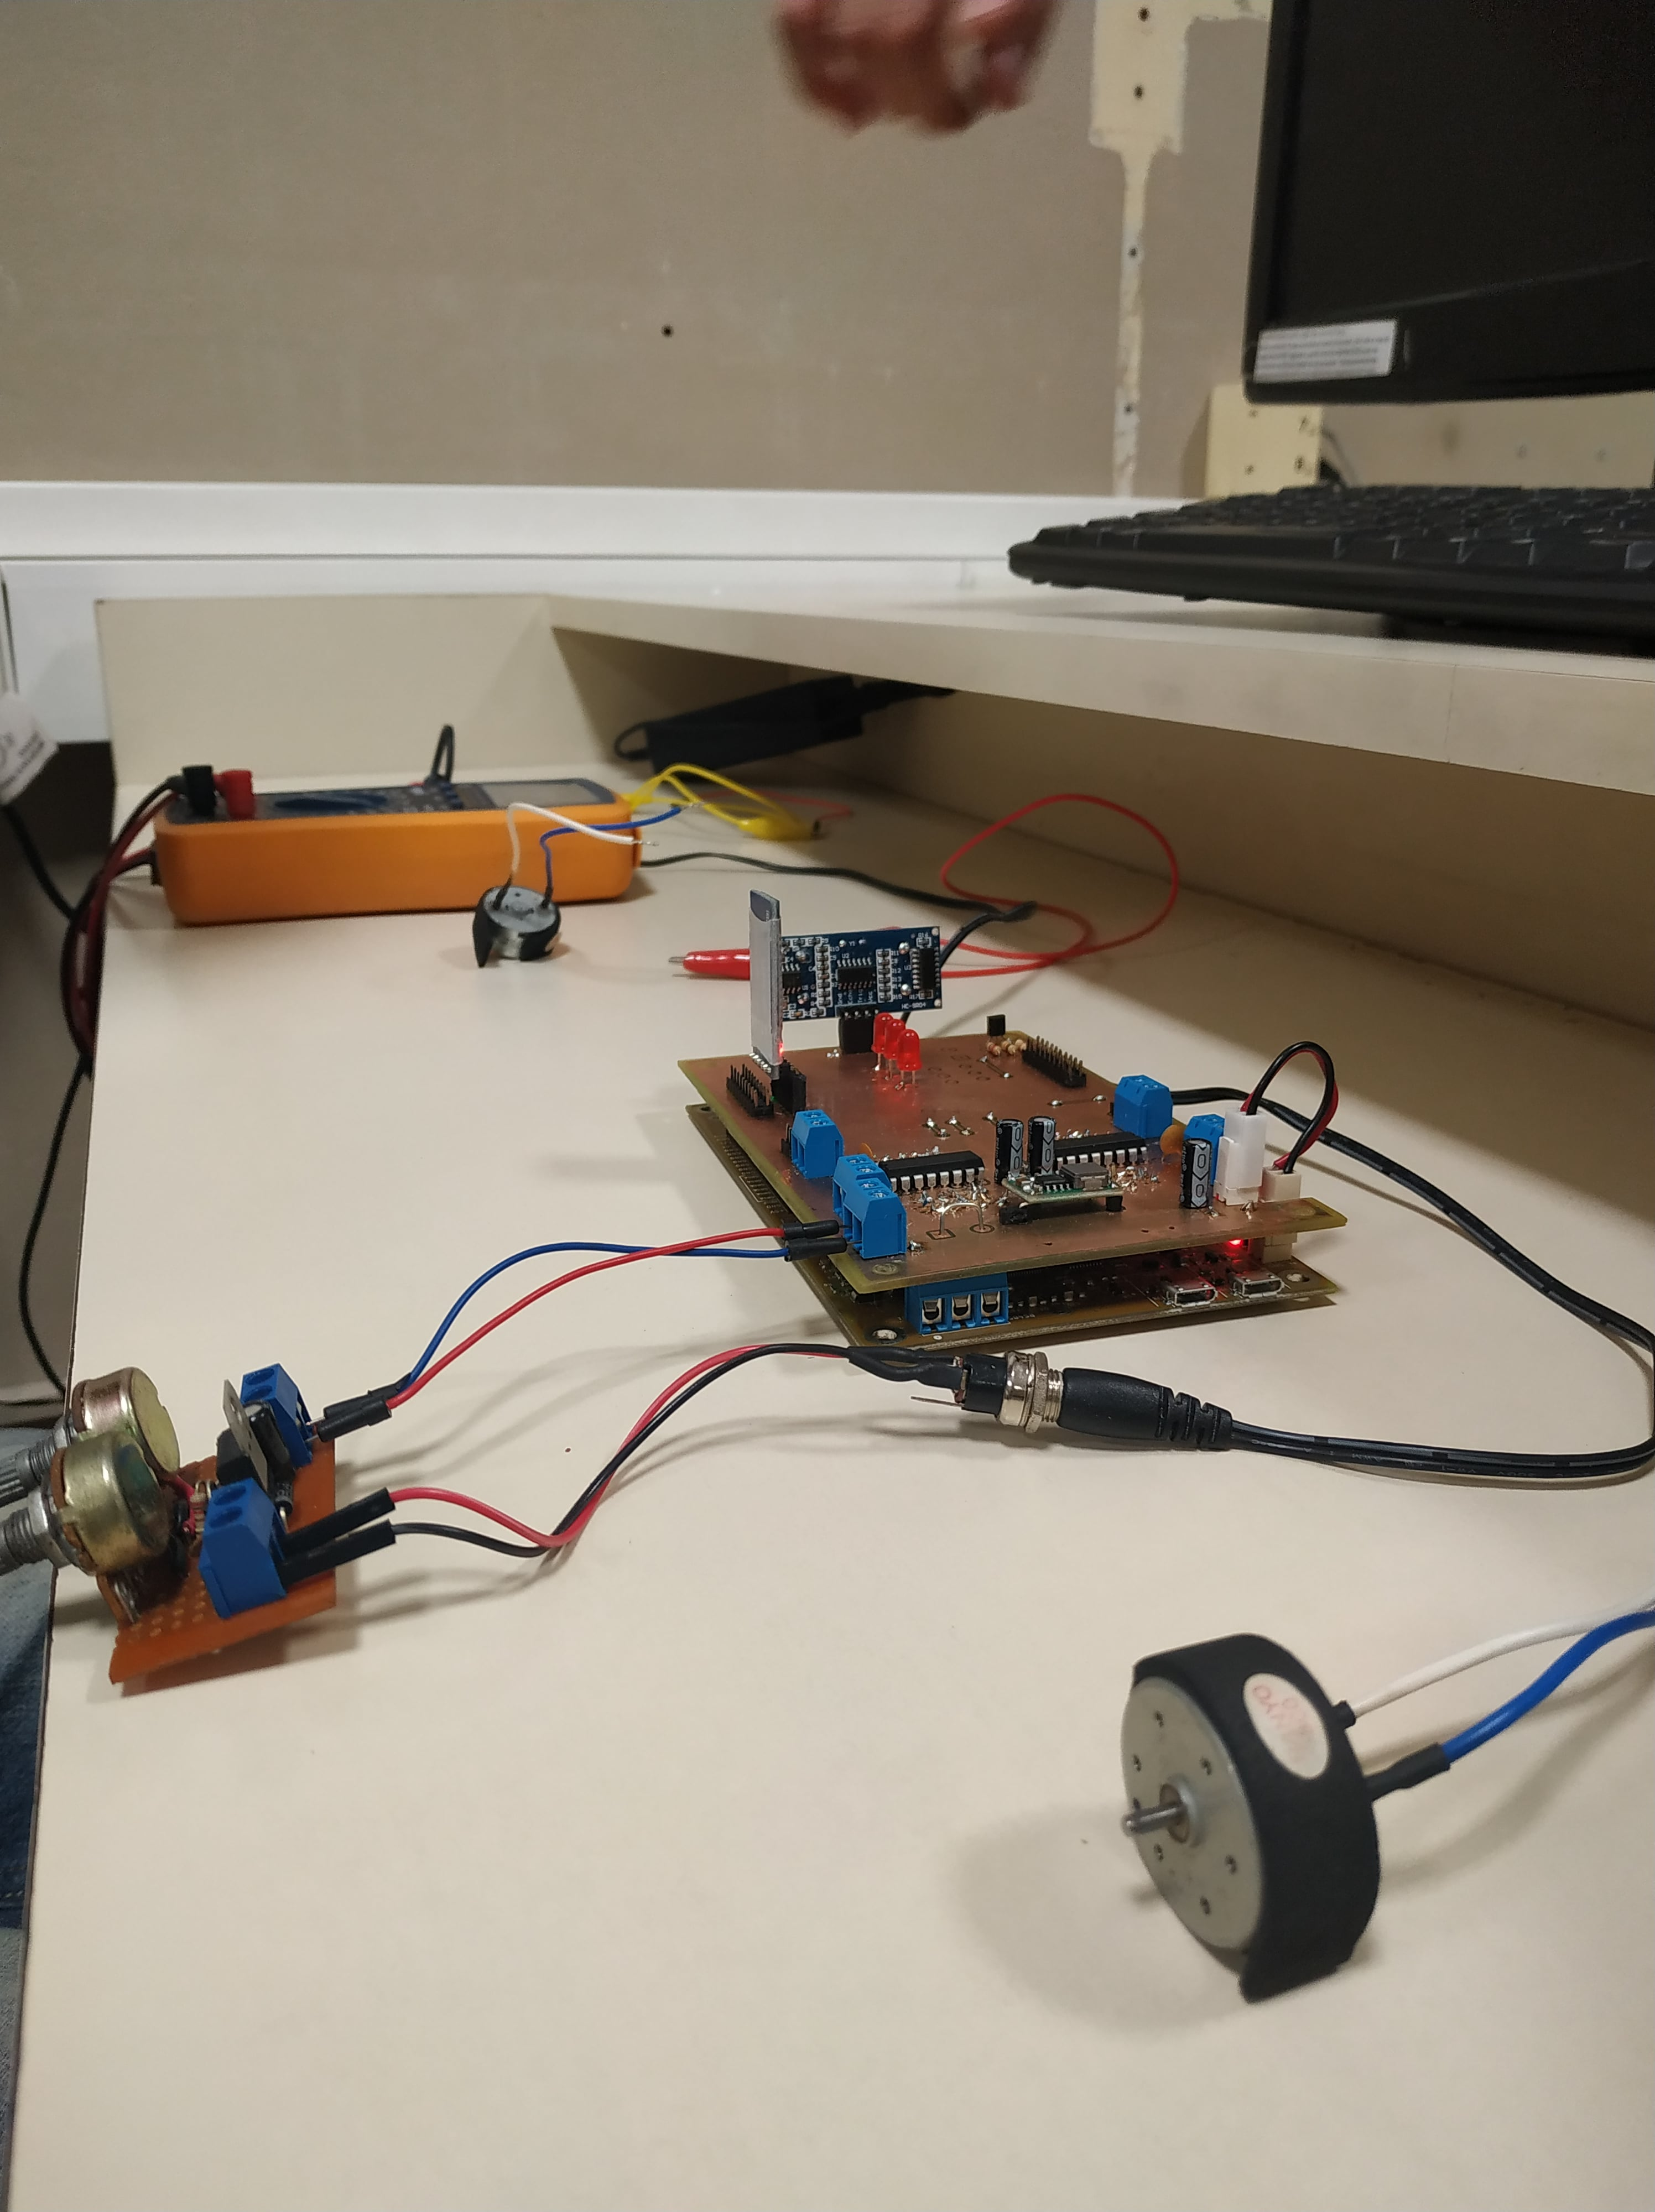
\includegraphics[width=1\linewidth]{imagenes/testing1.jpg}
	\label{fig:testing1}
\end{figure}

\begin{figure}[H]
\centering
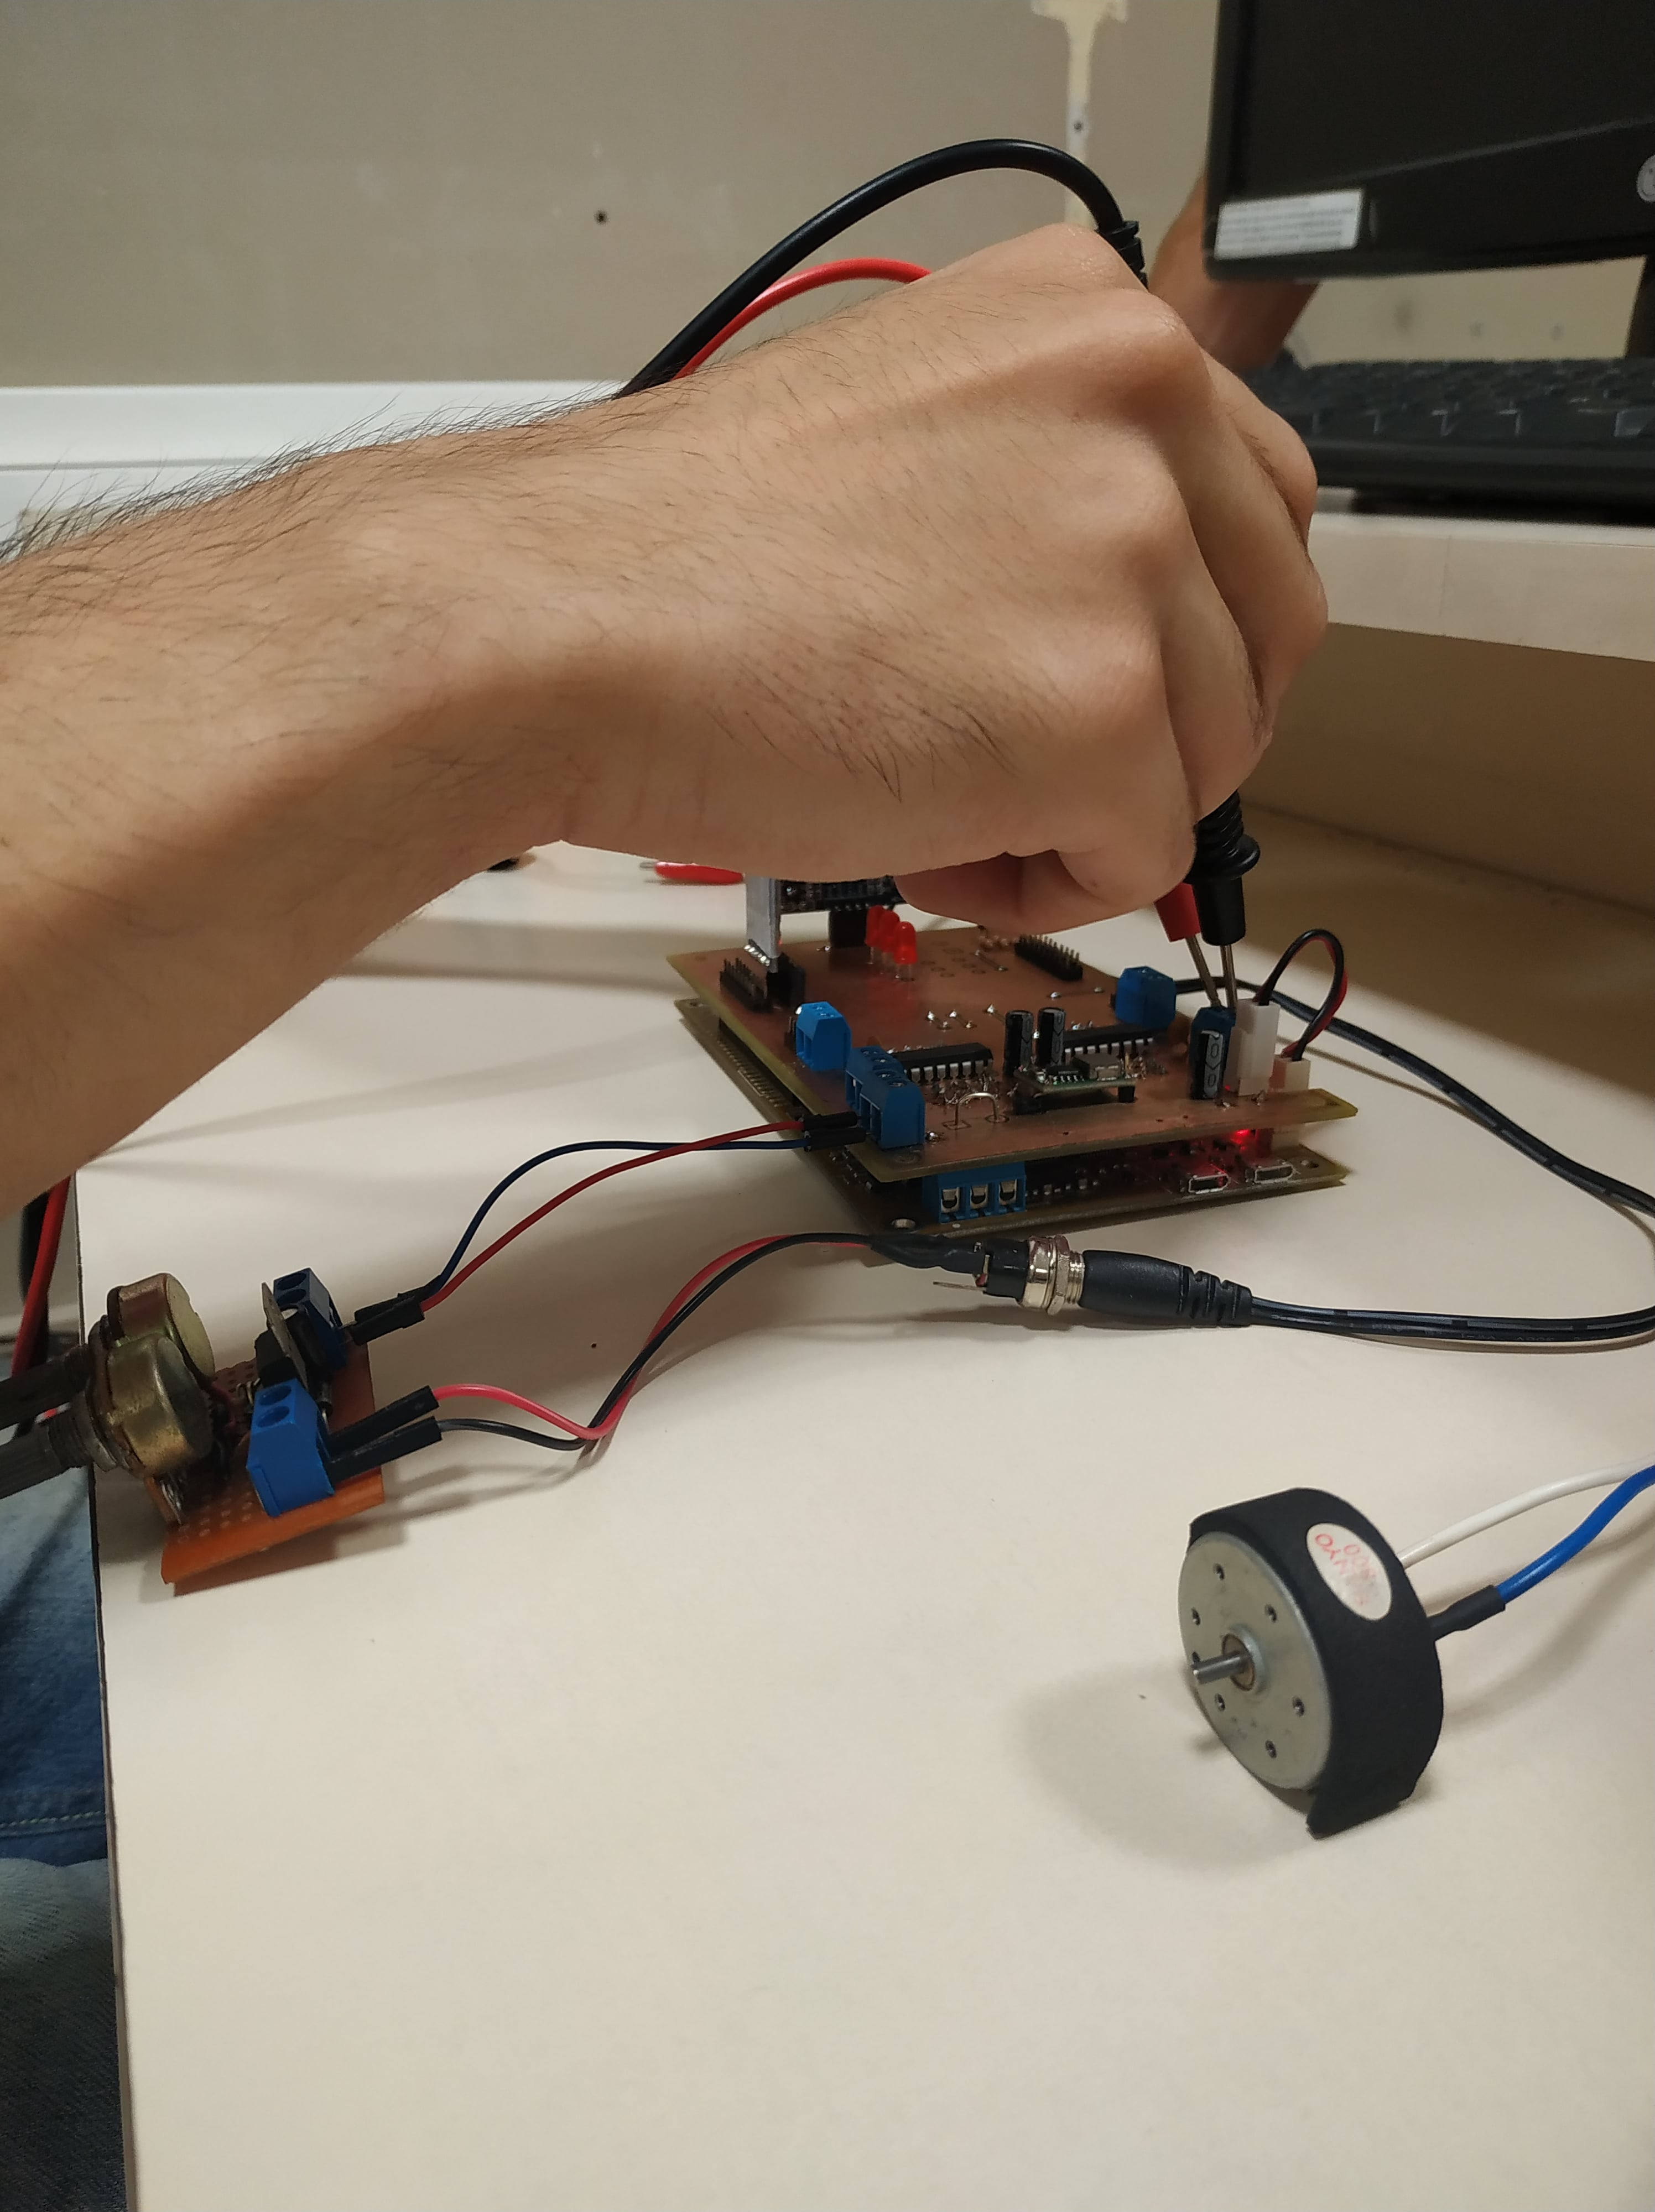
\includegraphics[width=1\linewidth]{imagenes/testing2.jpg}
\label{fig:testing2}
\end{figure}

\begin{figure}[H]
\centering
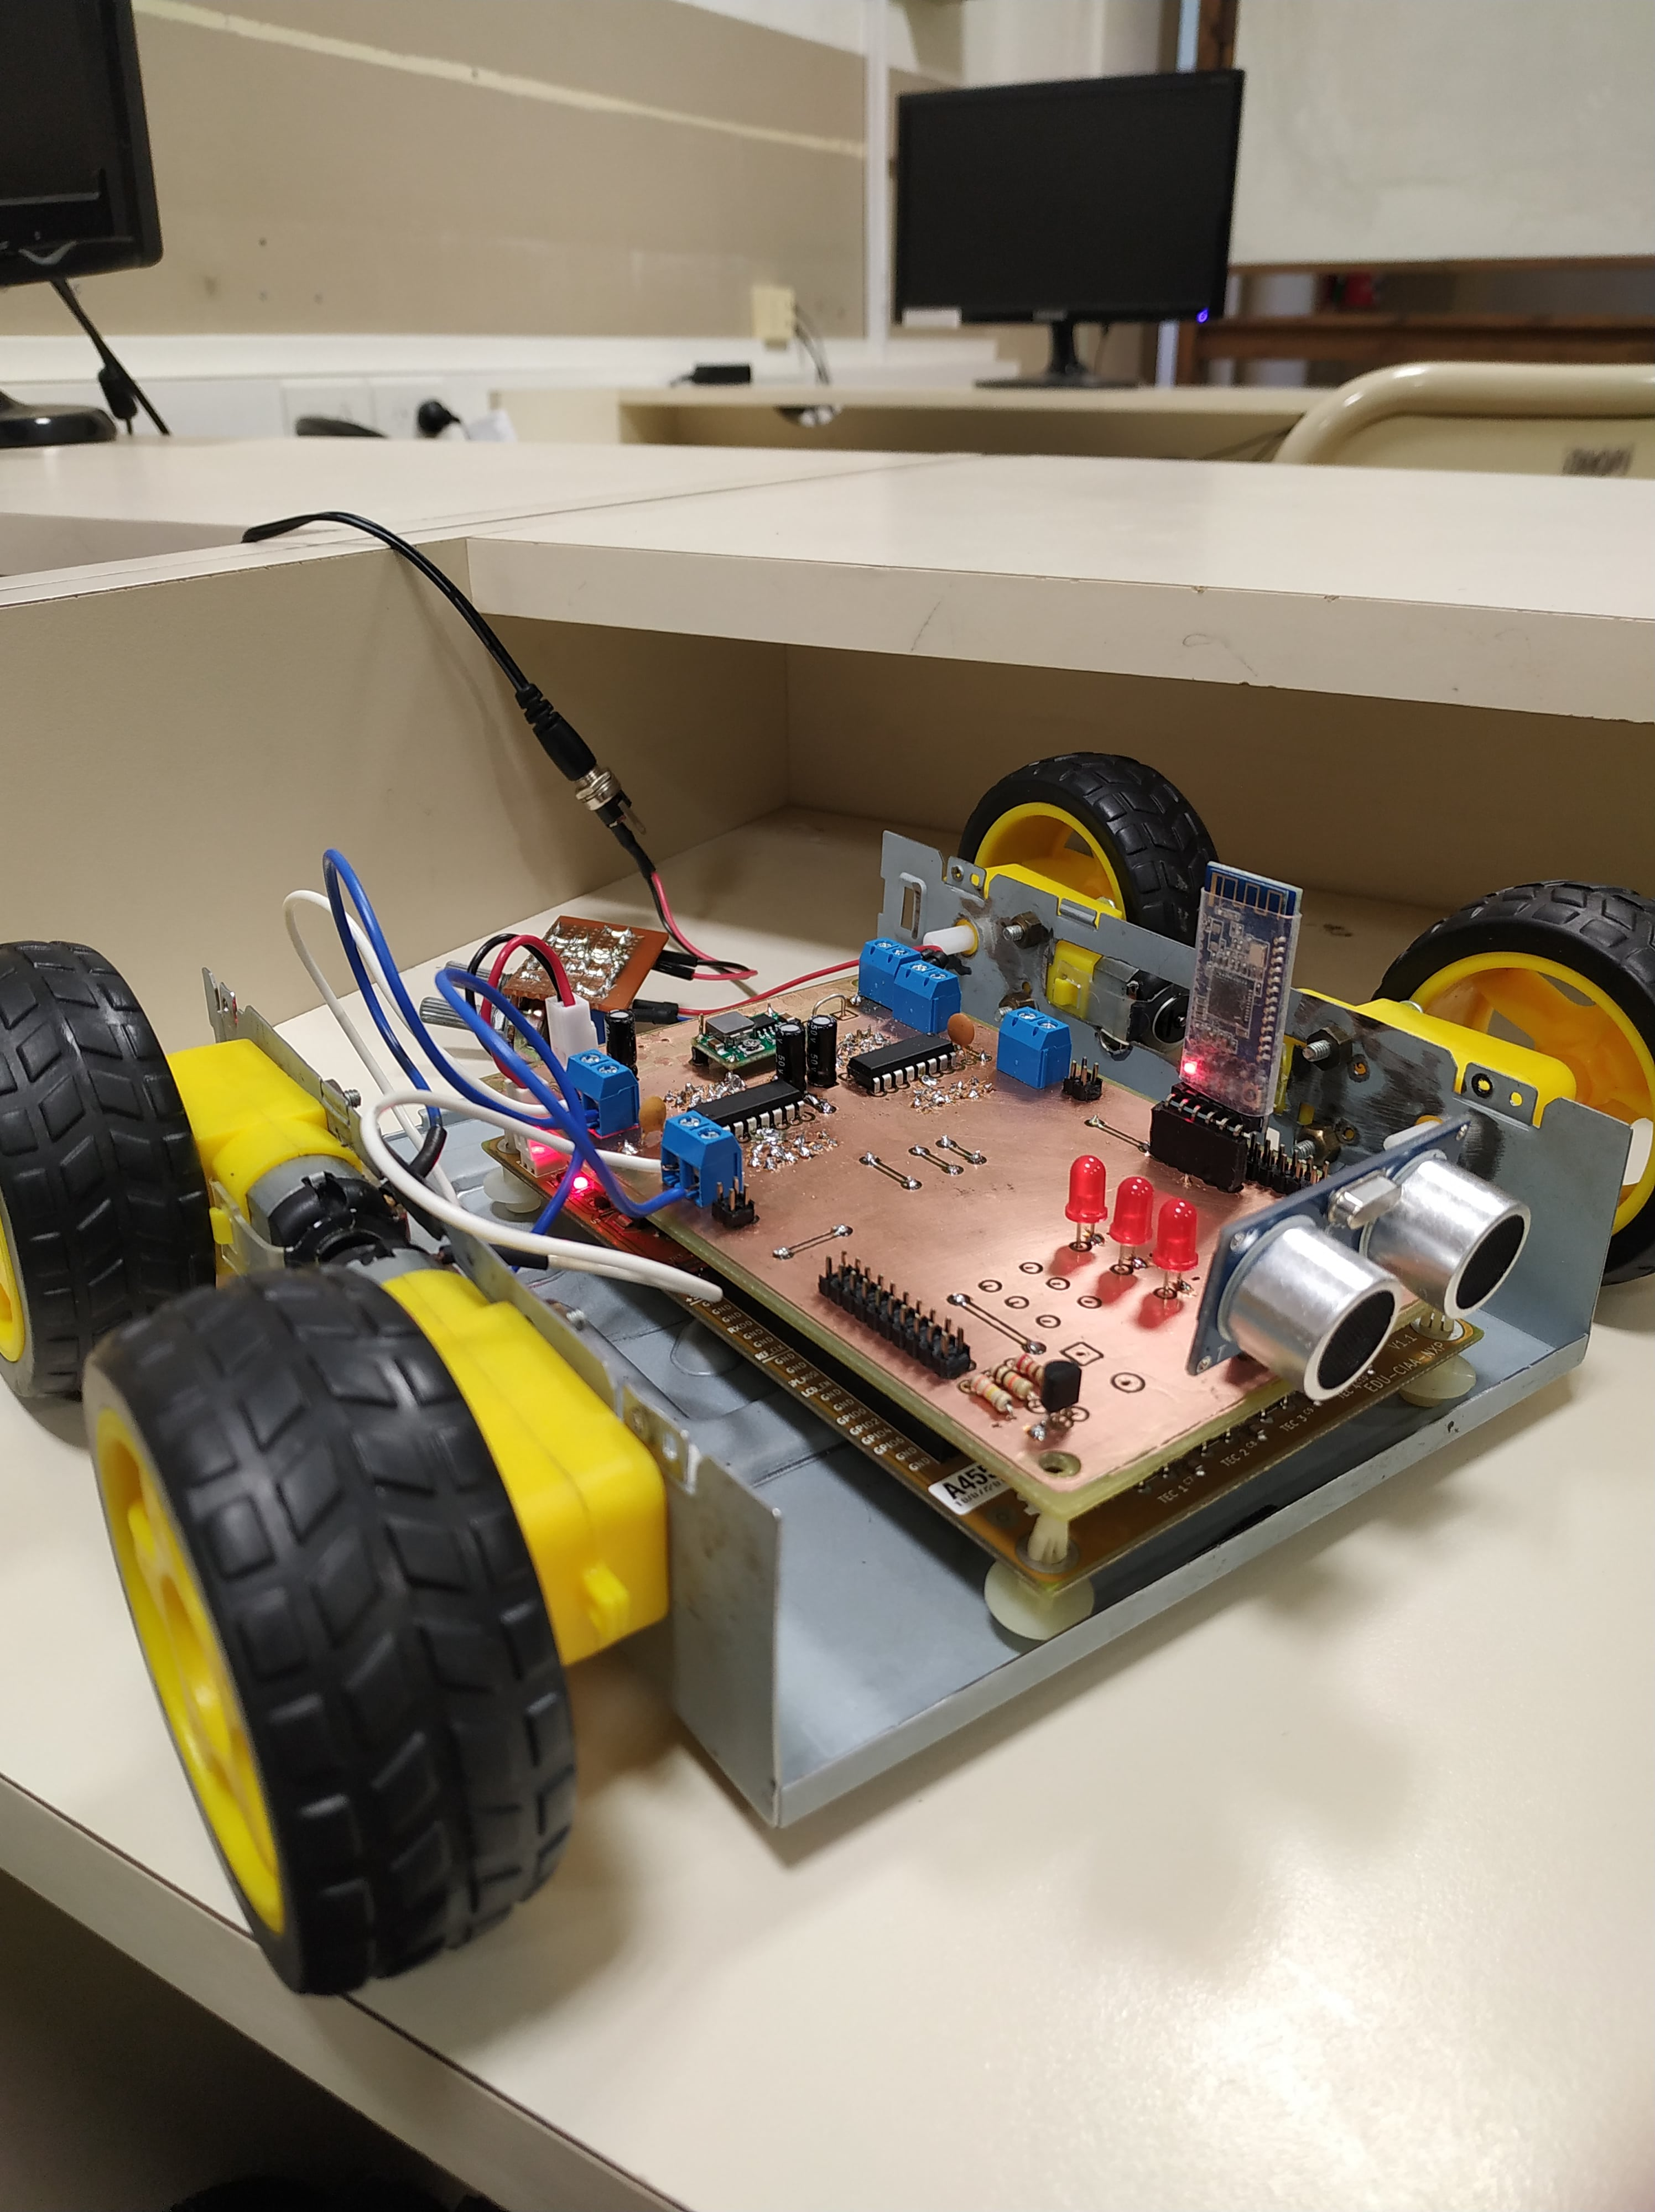
\includegraphics[width=0.9\linewidth]{imagenes/final_con_fuente_reguladora.jpg}
\label{fig:final5}
\end{figure}

\subsection{Proyecto terminado}

\begin{figure}[H]
	\centering
	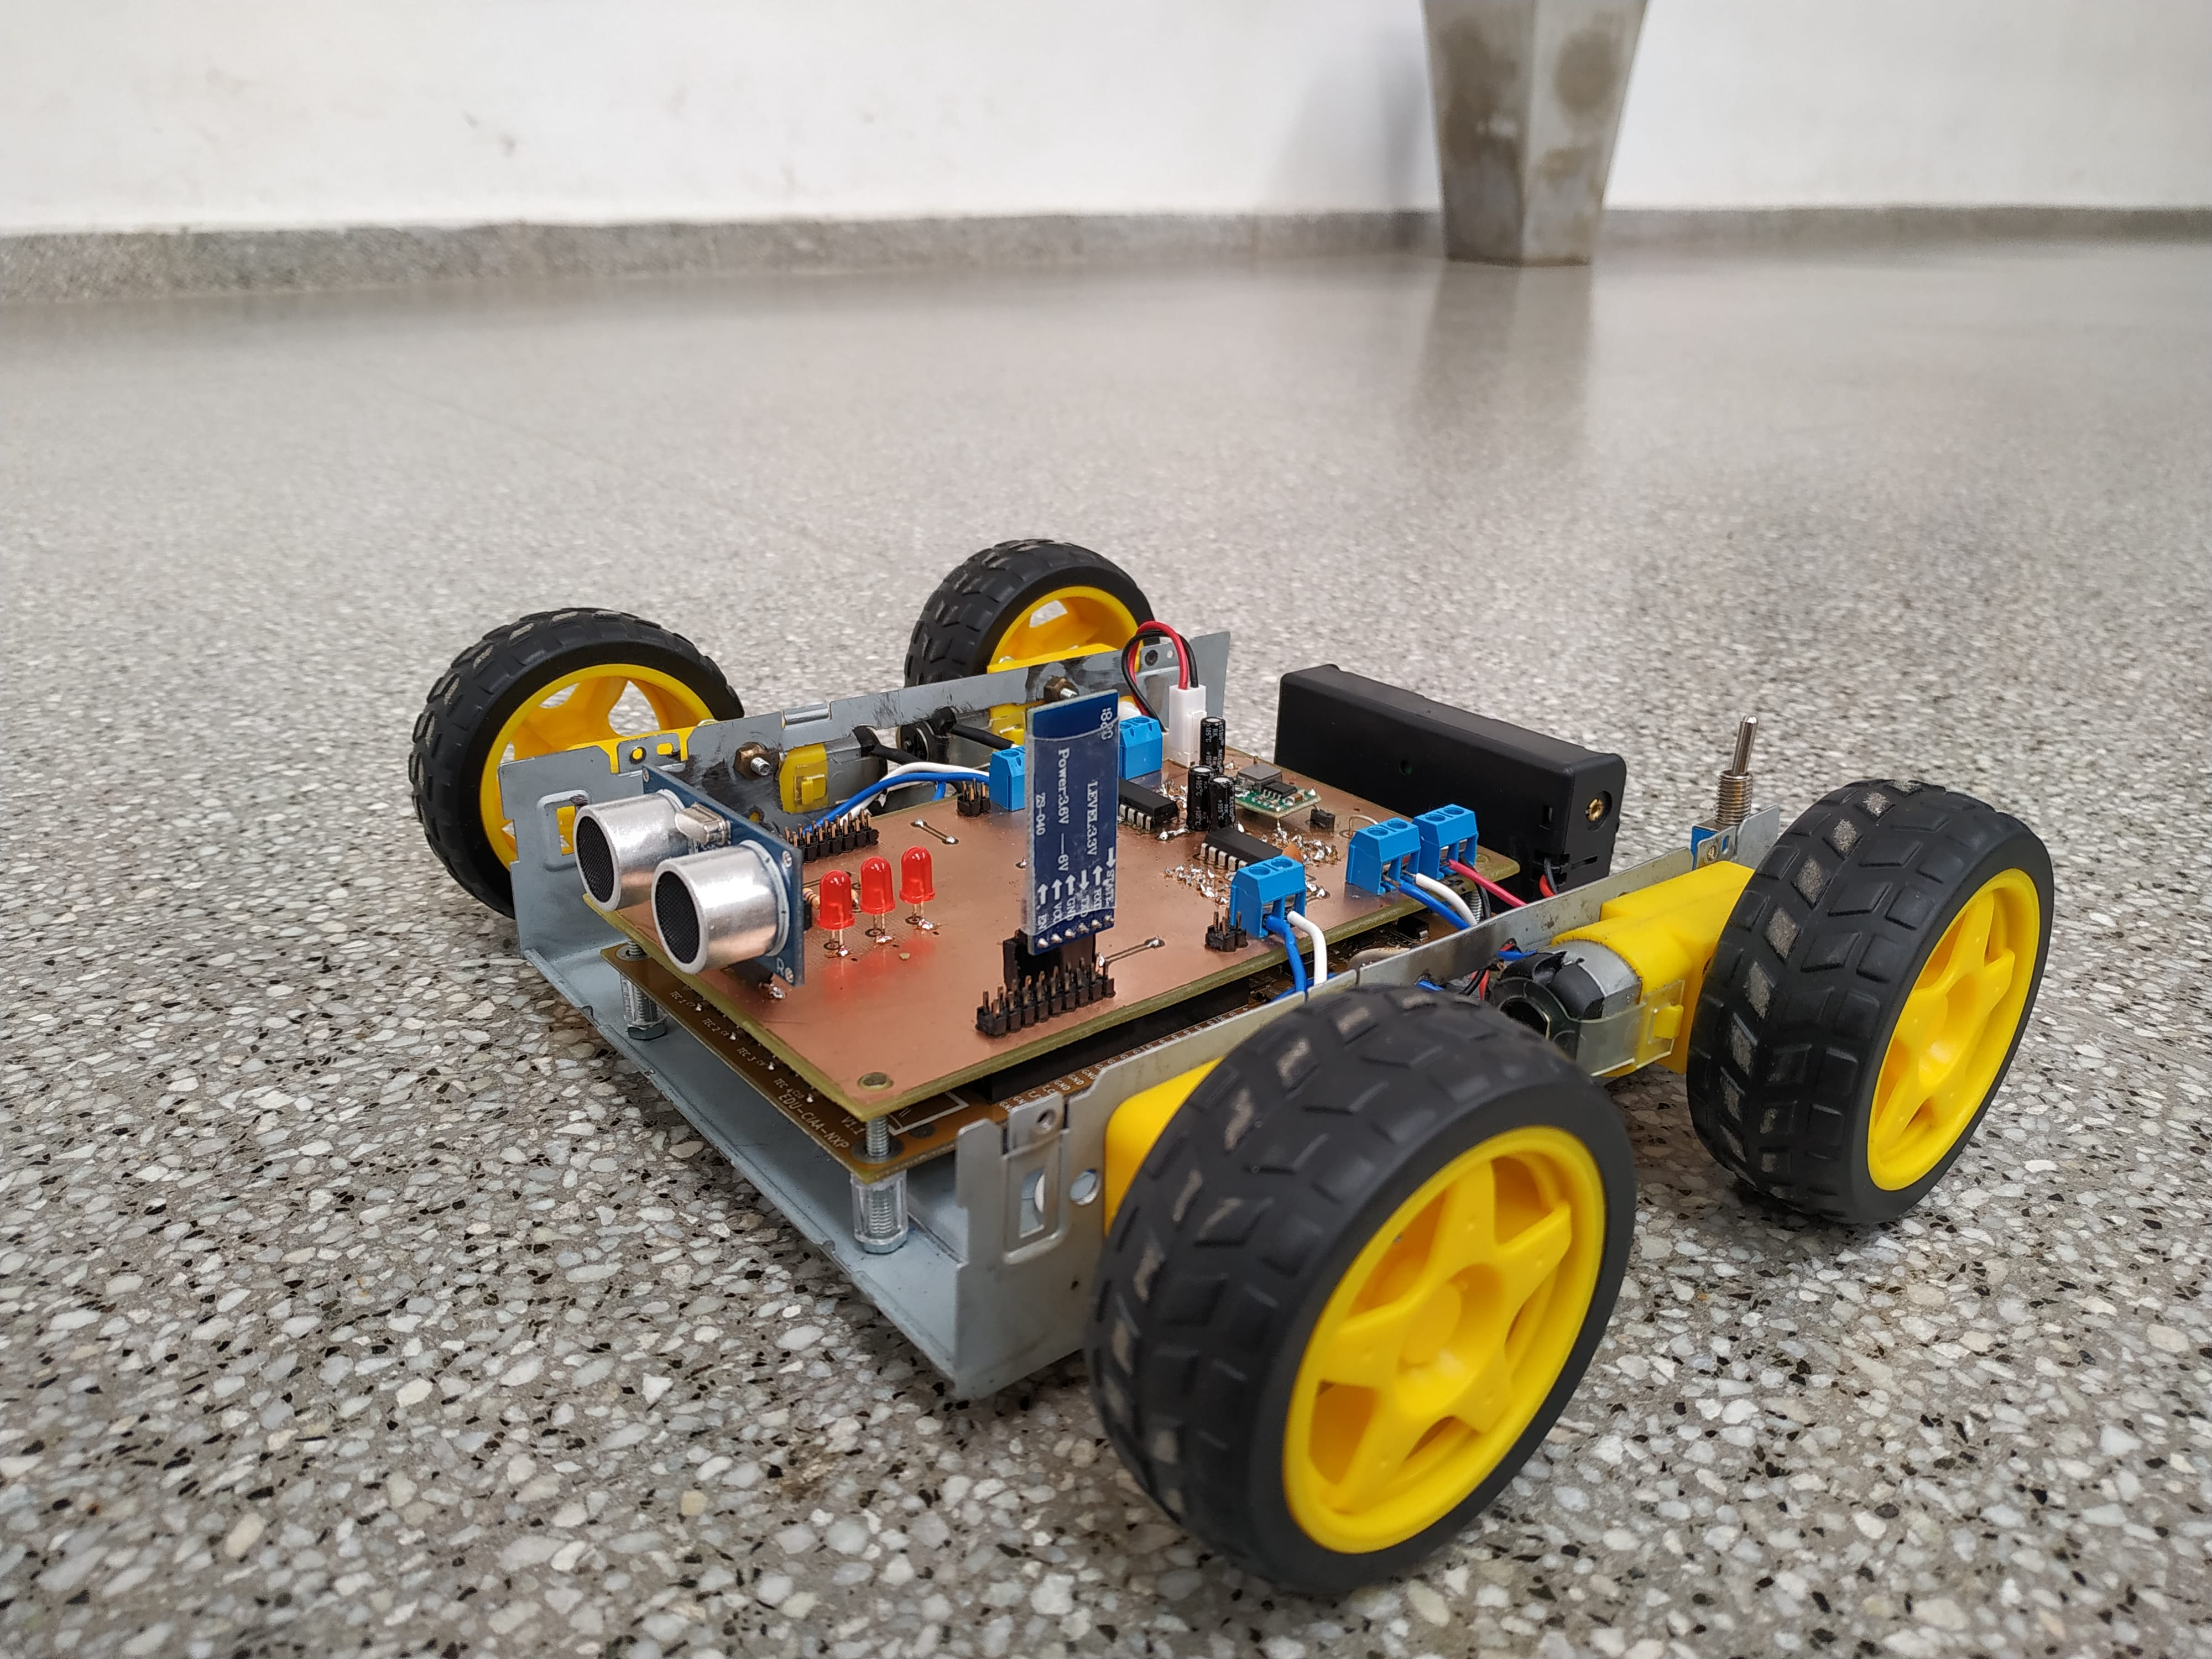
\includegraphics[width=0.9\linewidth]{imagenes/final4.jpg}
	\label{fig:final4}
\end{figure}

\begin{figure}[H]
\centering
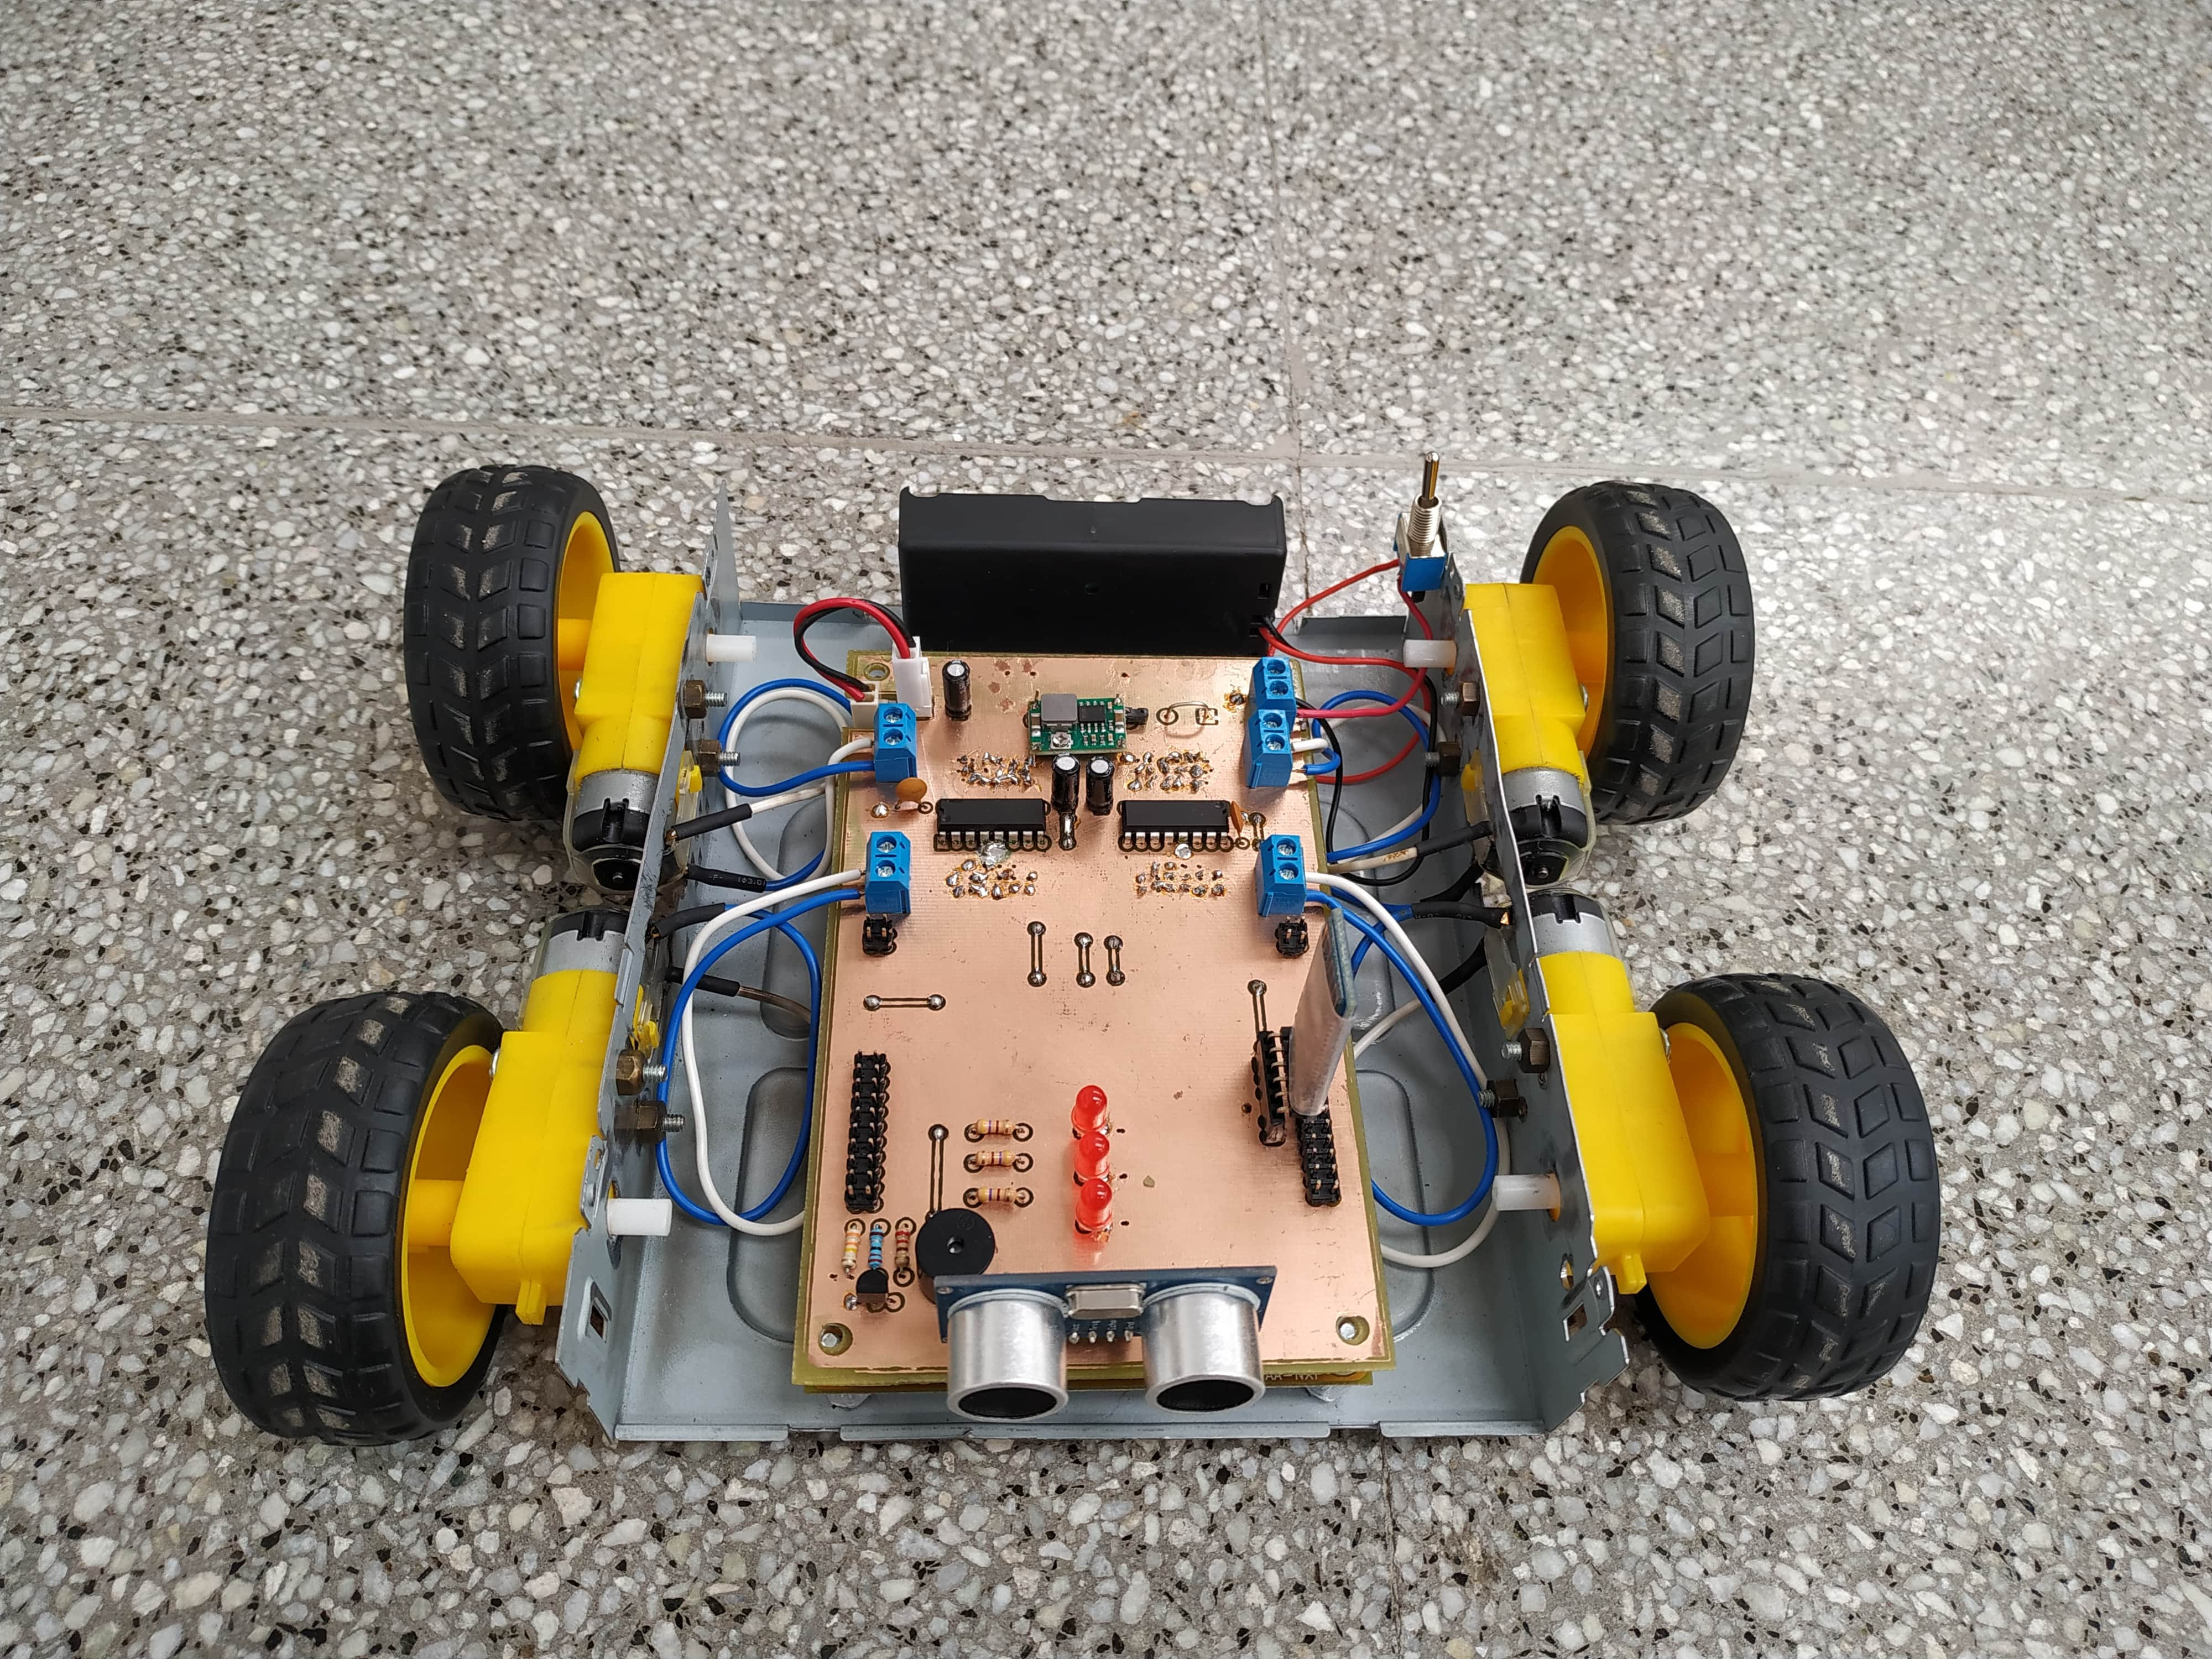
\includegraphics[width=0.9\linewidth]{imagenes/final2.jpg}
\label{fig:final2}
\end{figure}

\begin{figure}[H]
\centering
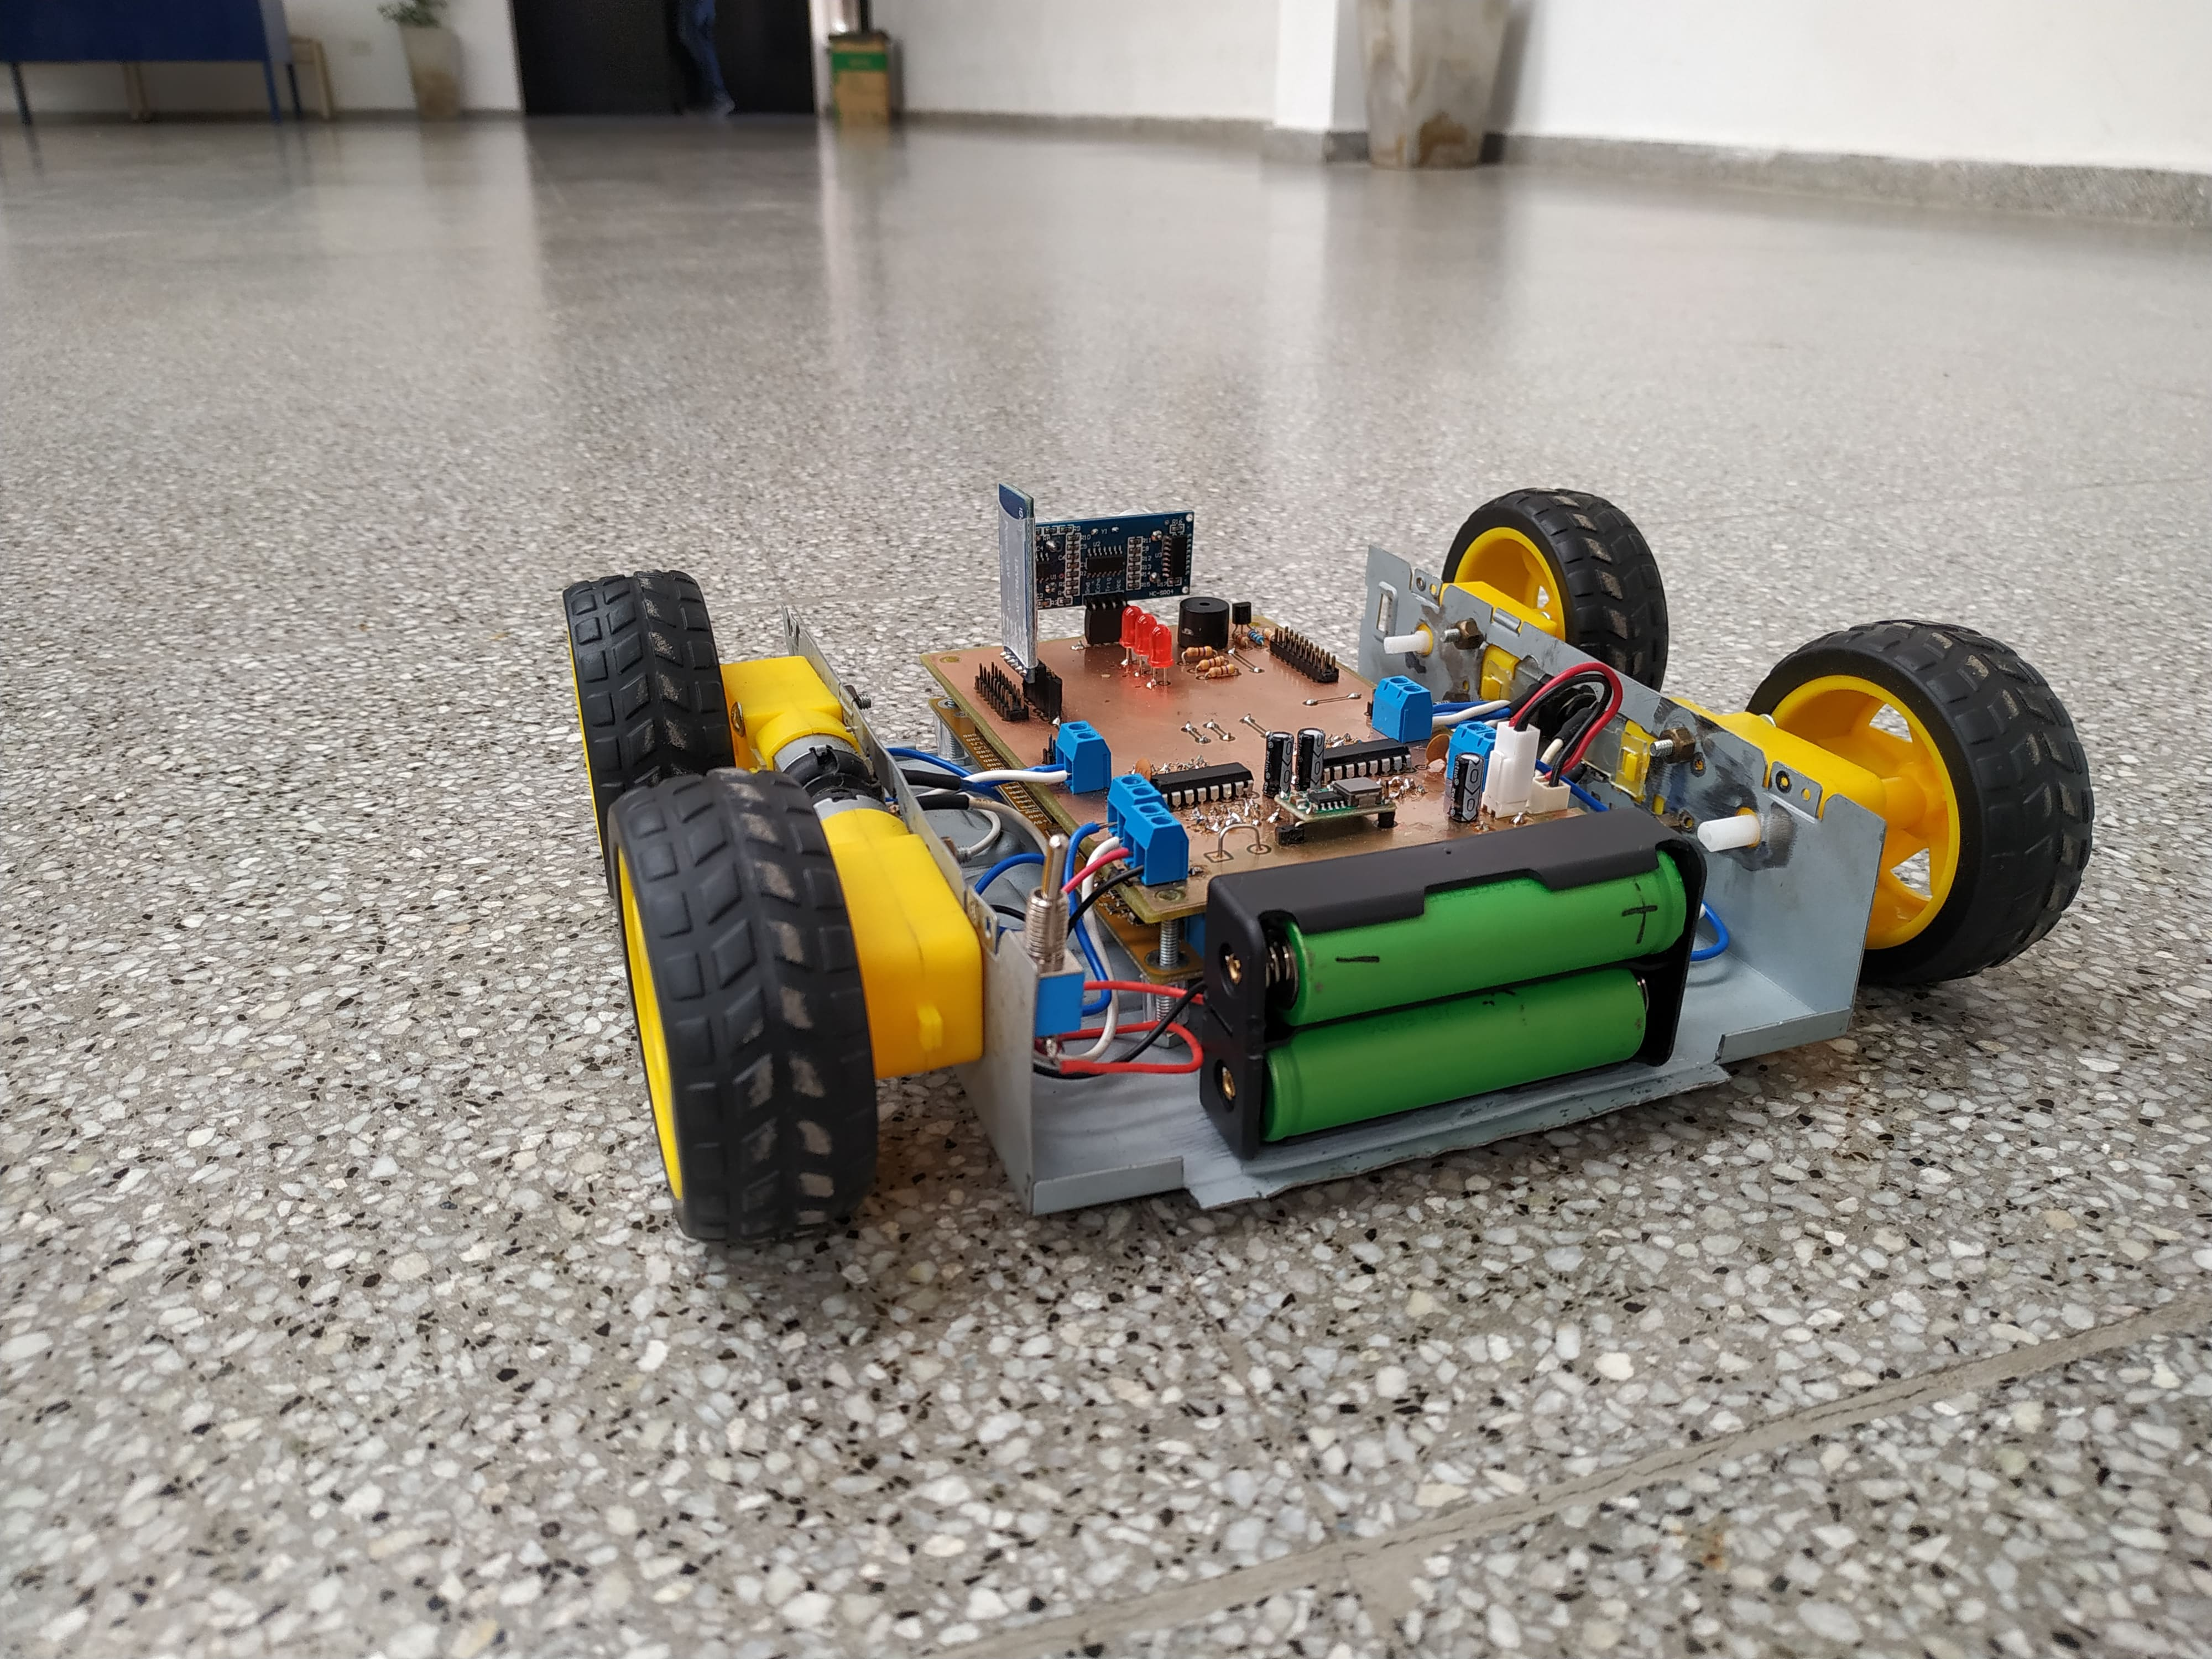
\includegraphics[width=0.9\linewidth]{imagenes/final3.jpg}
\label{fig:final3}
\end{figure}

\begin{figure}[H]
	\centering
	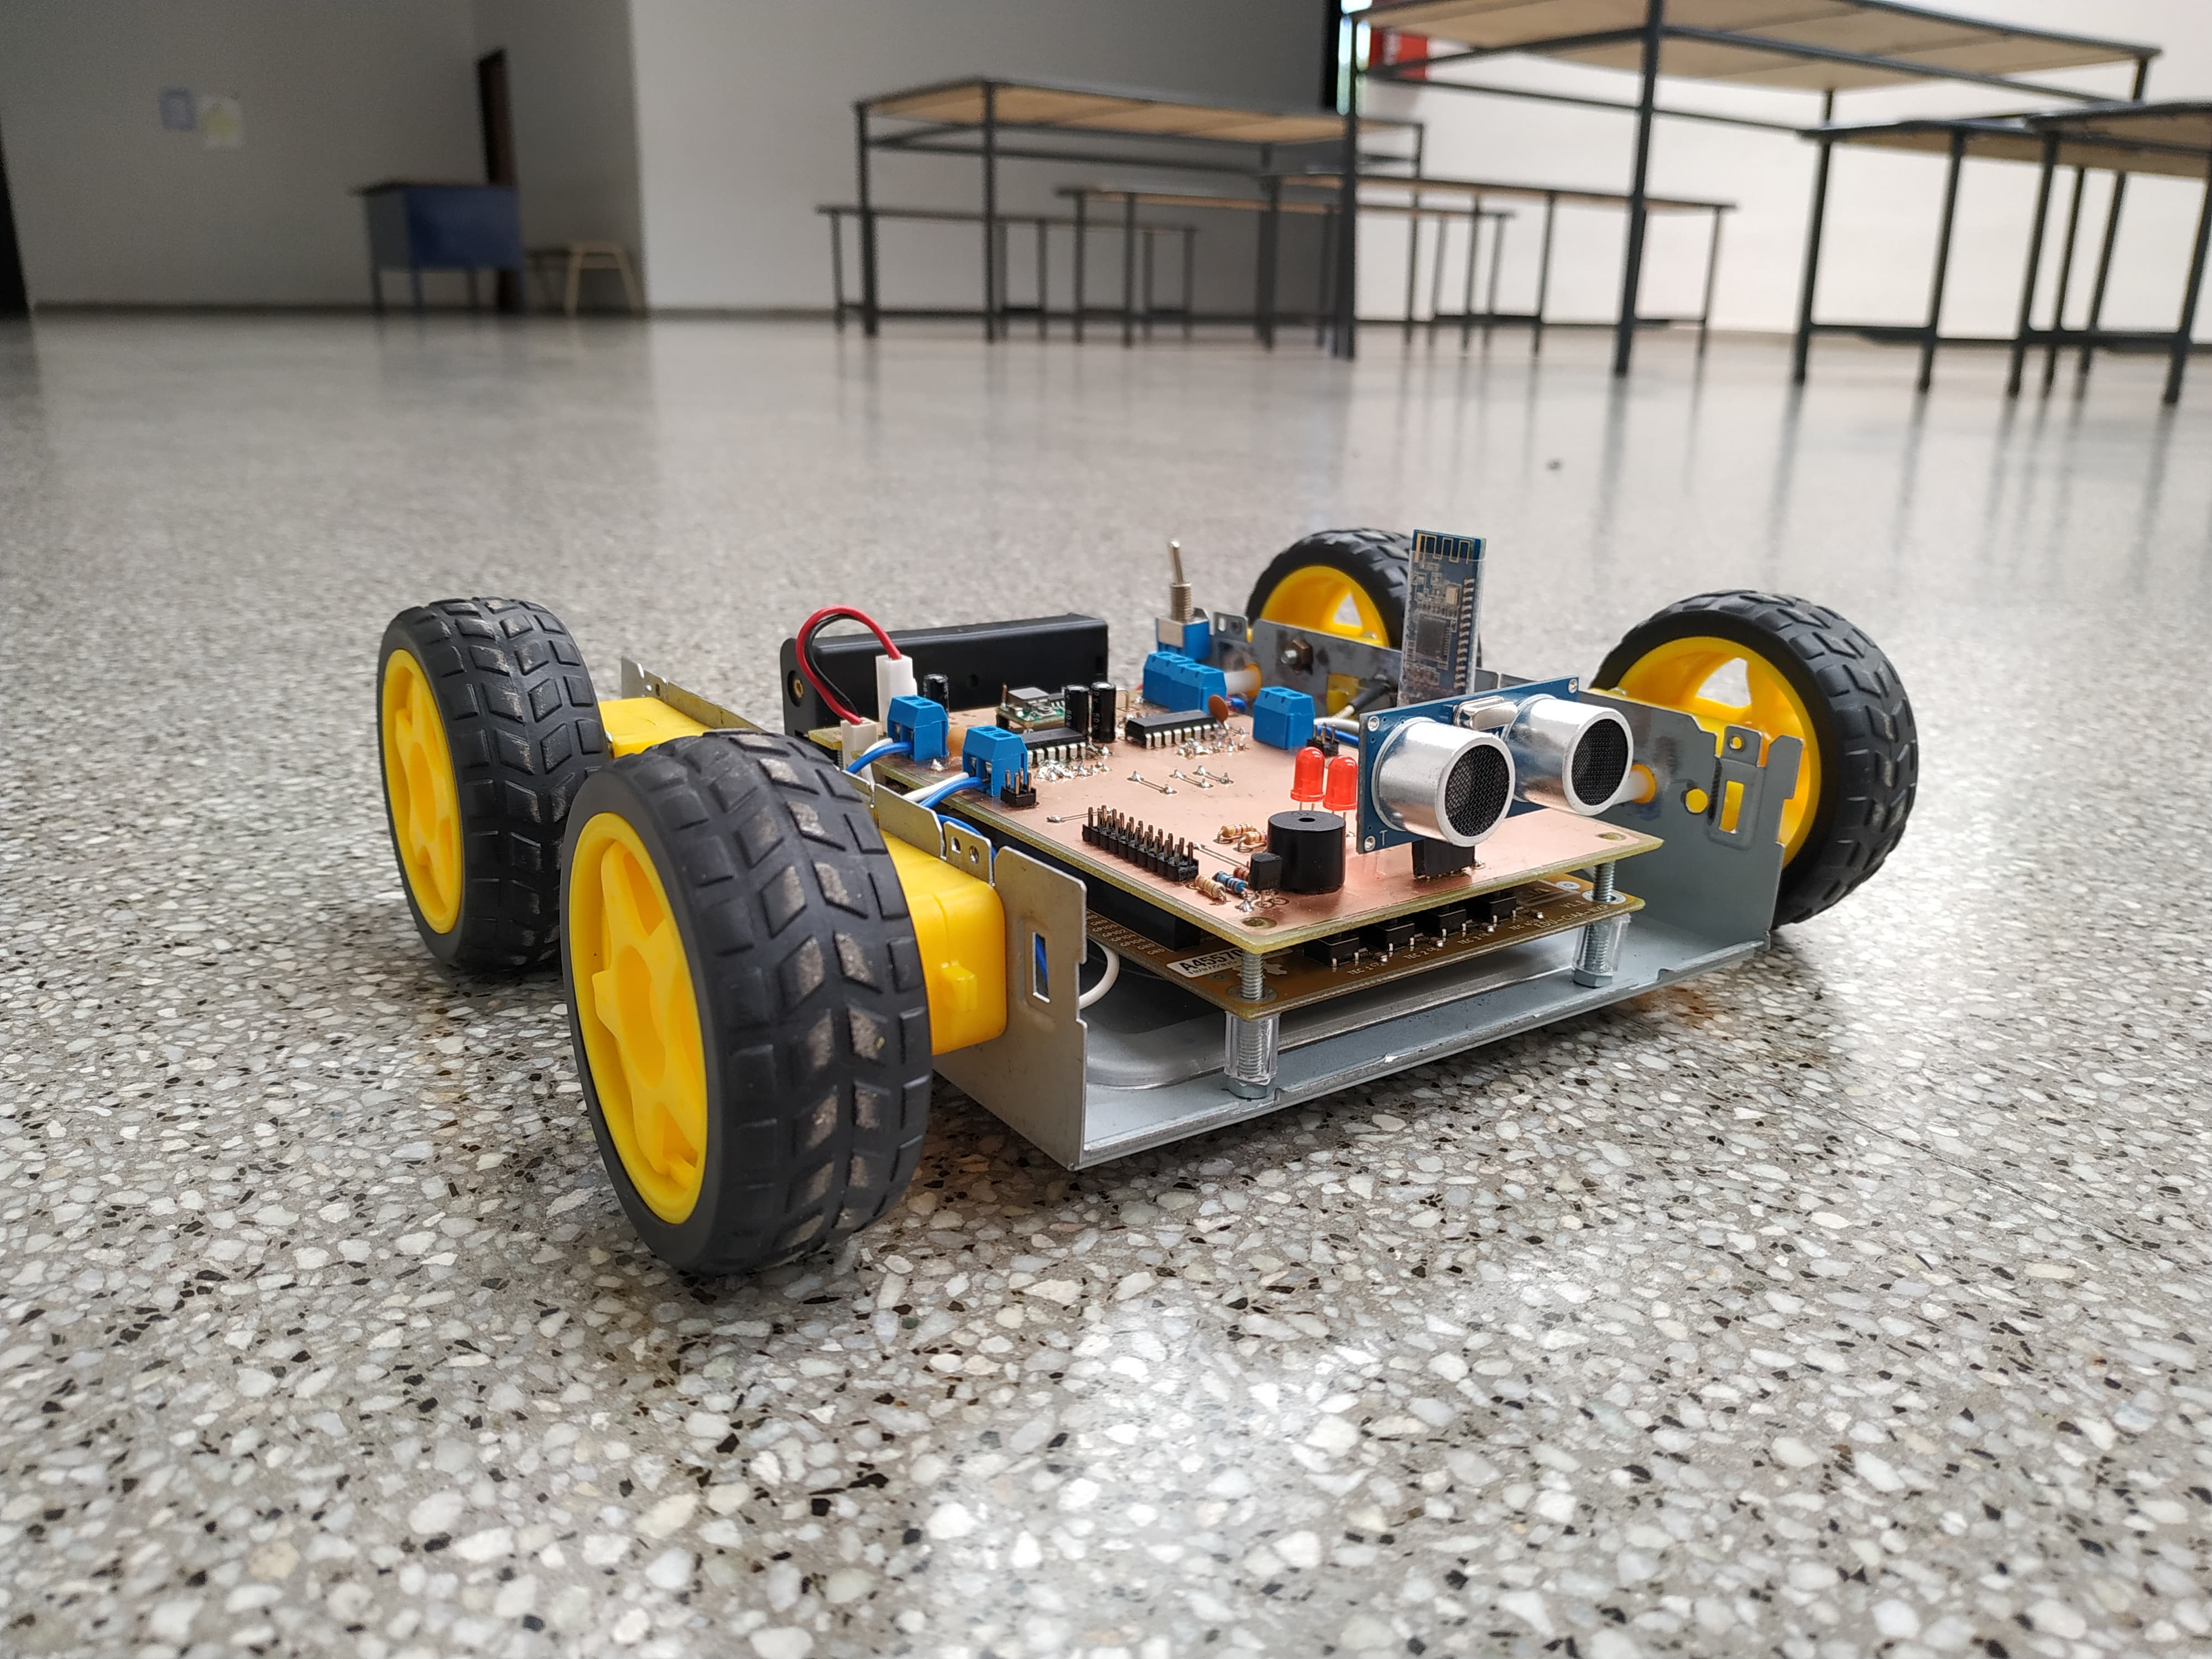
\includegraphics[width=0.9\linewidth]{imagenes/final1.jpg}
	\label{fig:final1}
\end{figure}

\begin{figure}[H]
	\centering
	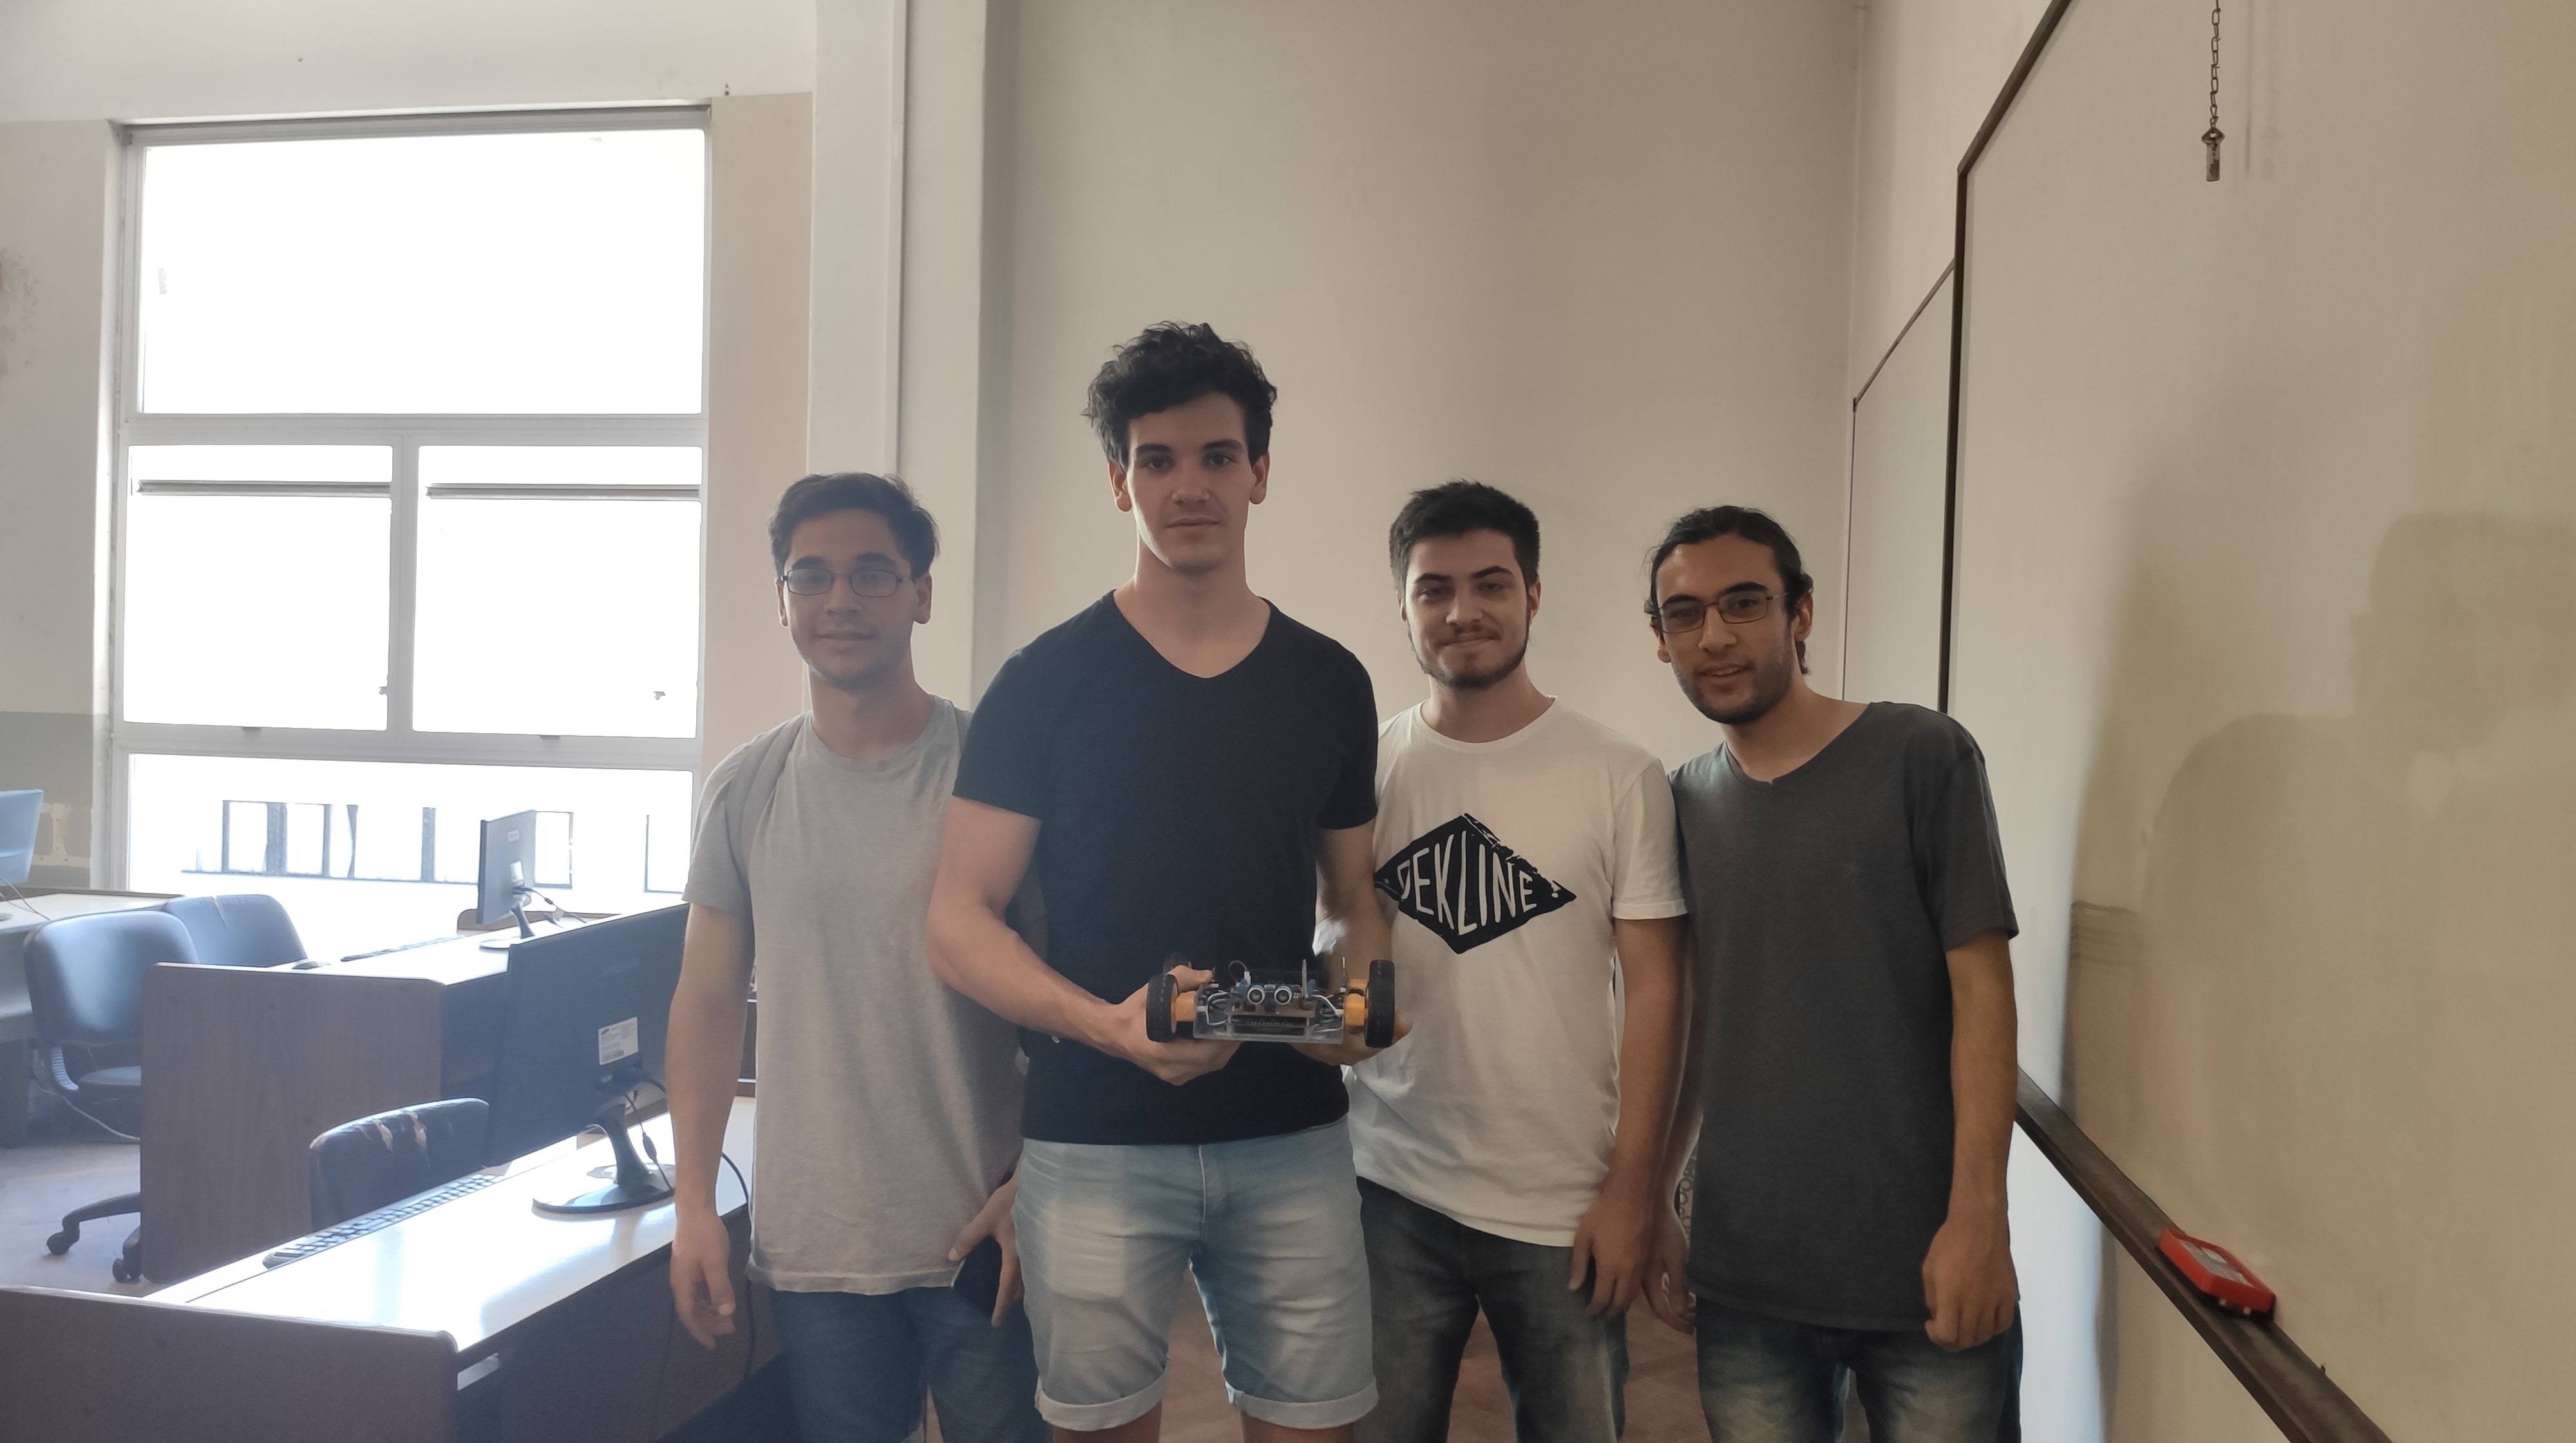
\includegraphics[width=0.9\linewidth]{imagenes/final6.jpg}
	\label{fig:final6}
\end{figure}
\end{document}